\chapter{The Compact Muon Solenoid}
\label{cms_description_overview}

\begin{figure}[h]
   \centering
  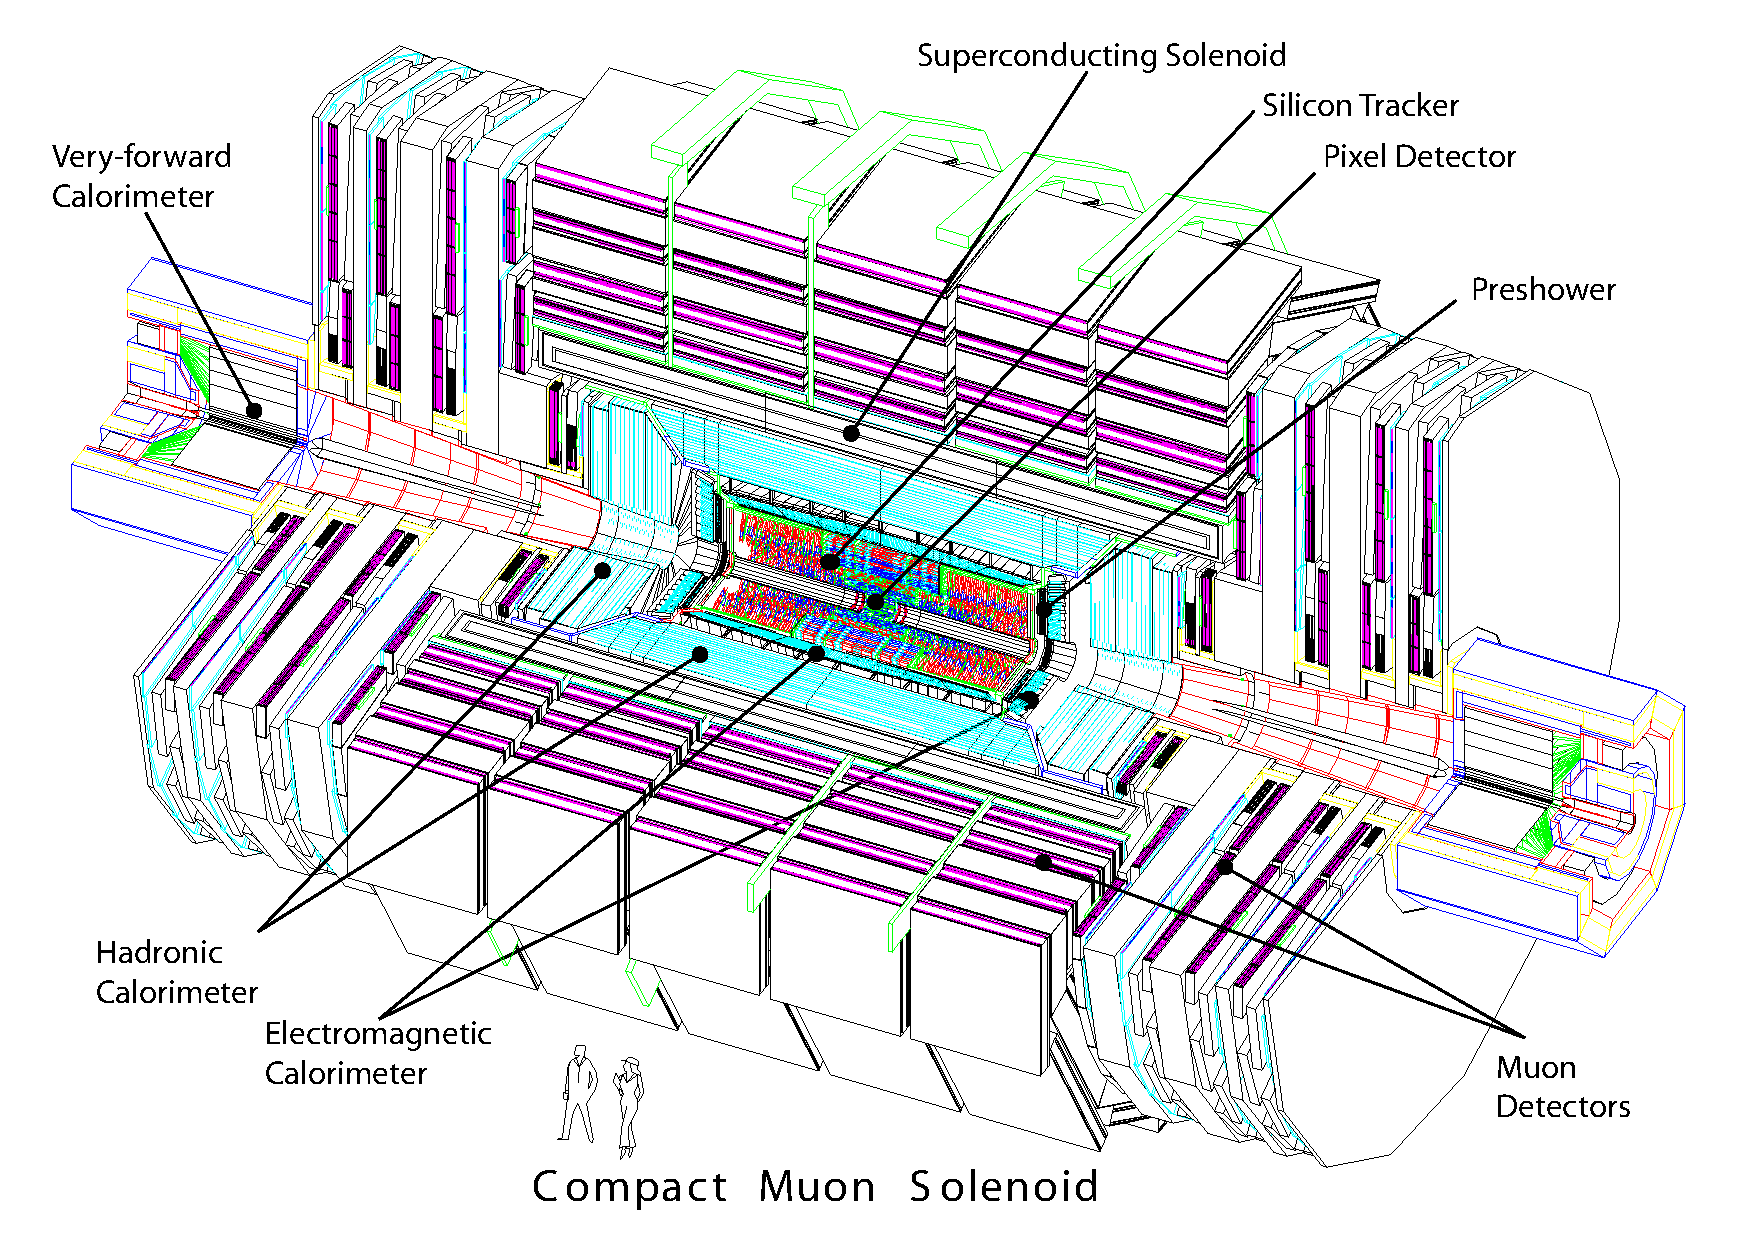
\includegraphics[width=0.7\textwidth]{Figures/CMS_Diagrams/CMS__Complete_Labelled.pdf}
  \caption{A cutaway diagram of the CMS detector.  Two humans are
    present at the bottom of the image to provide scale.} \label{fig:cms_complete}
\end{figure}

\par The \acrfull{cms} experiment is a general-purpose particle
detector capable of performing a wide range of physics measurements at
the \TeV energy scale.  It provides hermetic, $4\pi$, coverage
surrounding the interaction region on Point 5 of the LHC octant, and
is capable of identifying and reconstructing charged and neutral
hadrons, photons, electrons, and muons directly.  Tau leptons, are
measured indirectly through a careful reconstruction of its decay
products.  The hermetic coverage allows the detection of neutrinos by
measuring a momentum imbalance in a given collision.  The detector is
assembled in five sections and weights over 14,000 tons.  The
"Compact" part of the experiment's name comes from its relativley
small volume for a modern particle detector, with length of 28.7 m
and a diameter of 15.0 m.  Ironically, this is as tall as most 4-5
story buildings and weights as much as $\sim$7000 cars.  Figure
\ref{fig:cms_complete} shows a cutaway drawing of the CMS detector.  

\par A right-handed coordinate system is used to measure particle
positions within the detector.  The origin is centered at the nominal
interaction point with the $\hat{x}$ direction pointed towards the
center of the LHC ring, the $\hat{y}$ direction towards the sky, and
the $\hat{z}$ direction pointed counter-clockwise along the LHC ring
towards Point 2 and the ALICE experiment.  In the much more natural
polar coordinates, $\hat{r}$, points radially outward from the
interaction point, the azimuthal angle $\hat{\phi}$ is measured as the
angle relative to the $\hat{x}$ axis, and the polar angle,
$\hat{\theta}$, is measured as the angle relative to the $\hat{z}$
axis.  An important lorentz invariant position variable is the
rapitity, $y$, and its approximation in terms of the polar angle, the
pseudorapidity, $\eta$:

\begin{equation}
\begin{aligned}
y =&~ \frac{1}{2}\ln\left({\frac{E+p_{z}c}{E-p_{z}c}}\right) \\
\eta =&~ -\ln\left(\tan{\frac{\theta}{2}}\right)
\end{aligned}
\end{equation}

\noindent The psuedorapidity is useful since it is an approximately lorentz
invariant version of polar angle, which allows for a more intuitive
understanding of the distribution of particles when boosting into
different measurement reference frames.  The component of the momentum
transverse to the beamline, $p_{T}$ is the most common form of
measuring the momentum, and is defined as $p_{T} = |p|\cos{\phi}$.  

\begin{figure}[h]
   \centering
  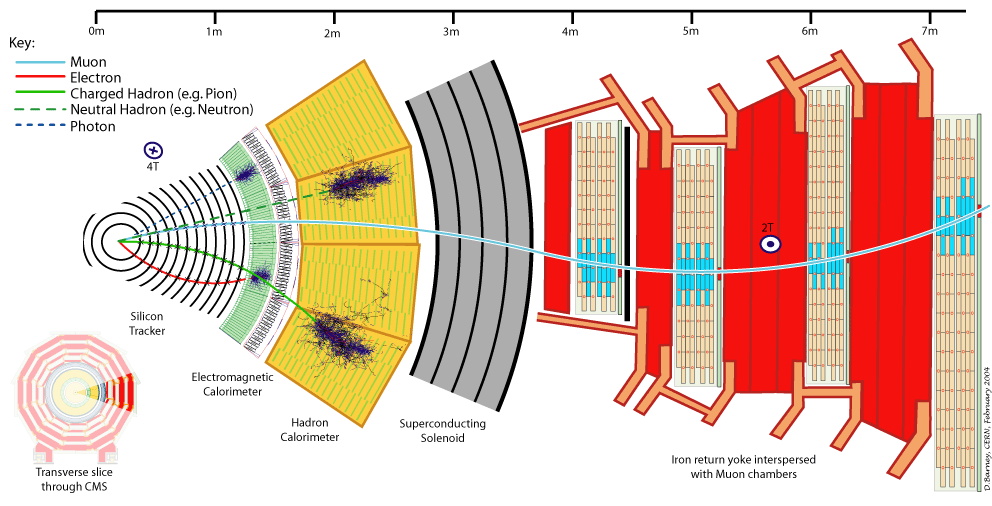
\includegraphics[width=0.9\textwidth]{Figures/CMS_Diagrams/CMS__Slice.png}
  \caption{A slice of the CMS detector showing how various particles
    interact and deposit energy.  The trajectory of charged particles
    is measured in the tracker; electrons and photons deposit most of
    their energy in the ECAL; charged and neutral hadrons deposit most
  of their energy in the HCAL; the muon chambers measures the
  trajectory of muons or long-lived charged particles} \label{fig:cms_slice}
\end{figure}

\par CMS is composed of a system of sub-detectors, each
specialized in measuring a certain type or characteristic of a
particle.  They are arranged approximately as concentric cylinders of
increasing radius, wrapped around the interaction region of the $pp$
collisions and an analogy is often made between the layers of
subdetectors being similar to the layers of an onion. The closest 
sub-detector to the interaction region is the tracker system.  It is
an all silicon pixel and strip detector, with a high precision 
position resolution, which is used to identify the trajectory of
charged particles close to the primary vertex of a collision.  The
\acrfull{ecal} is the next layer, and is used to absorb energy of
electromagnetically interacting particles.  It uses lead-tungstate
(PbWO$_{4}$) crystals which act as both the absorbing and scintilating
medium for energy deposited by charged particles and photons as they
pass through  this sub-detector.  The \acrfull{hcal} uses brass and
steel tiles to absorb energy and induce hadronic interactions, while a
plastic scintillator material layered between the absorber tiles
samples the energy of hadrons.  The tracker, ECAL, and HCAL systems
are all contained in the bore of the 3.8 T solenoid from the CMS
namesake.  This device bends the trajectory of charged particles as
the traverse the detector, and the curvature of this bend is used to
obtain information on the charge and momentum of the measured
particle.  The muon system sits outside of the solenoid structure, and
uses three types of detection systems: drift tubes (DTs), resistive
strip chambers (RPCs) and cathode strip chambers (CSCs), which provide
excellent timing and position resoultion.  The retun yoke structure of
the magnet also provides the mechanical support for the muon
chambers.  Figure \ref{fig:cms_slice} shows a slice of the CMS
experiment showing how various particles ineract and traverse the different
sub-detector regions, as descirbed above.  

\par At center-of-mass energy of $\sqrt{s}=14 \TeV$, the expected
event rate is approximately 10$^{9}$ events/second.  This is too much
information to store and analyze, and is maninly dominated by Standard
Model QCD multi-jet production, a background for searches for new
particles or physics.  An online event selection, or trigger, must by
used to reduce this rate to a manageable 100 events/second.  This is
acheived through a combination of hardware, firmware, and software
that provides a rough reconstruction of events in near real-time, and
makes a decision about whether it meets a minimum set of criteria to
be used in an analysis.  


\section{The Tracker}
\label{tracker_description}

\par The innermost sub-detector is an all silicon pixel and strip
tracker designed to provide precise and efficient measurement of the
trajectories of charged particles and reconstruction secondary
vertices necessary for identification of $b$-jets and $\tau$ leptons.  

\par At peak LHC design luminosity of $10^{34}$cm$^{-2}$s$^{-1}$, and bunch
spacing of 25 ns, there will be $\sim$1000 particles from 20
overlapping $pp$ collisions for each bunch crossing.  This correspons
to a hit rate density of 1 MHz/mm$^{2}$ at a radius of 4 cm, 60
kHz/mm$^{2}$ at 22 cm, and 3 kHz/mm$^{2}$ at 115 cm from the beam
line.  This large particle flux will also cause intense radiation
damage to detector components.  These conditions necessitate the use
radiation-hard silicon, with a high-granularity to create a low
occupancy for each detector element, which are read out by fast
electronics. Additional mitiagation of the effects of radiation damage
is taken by cooling and operating the entire detector to -10$^{\circ}$
C in order to maintain a signal to noise ratio of 10:1 for the
sensors.  After 10 years of running, it is anticipated that this will
need to decrease to -27$^{\circ}$ in order to compensate for the
accumulated damage.    

\begin{figure}[h]
   \centering
  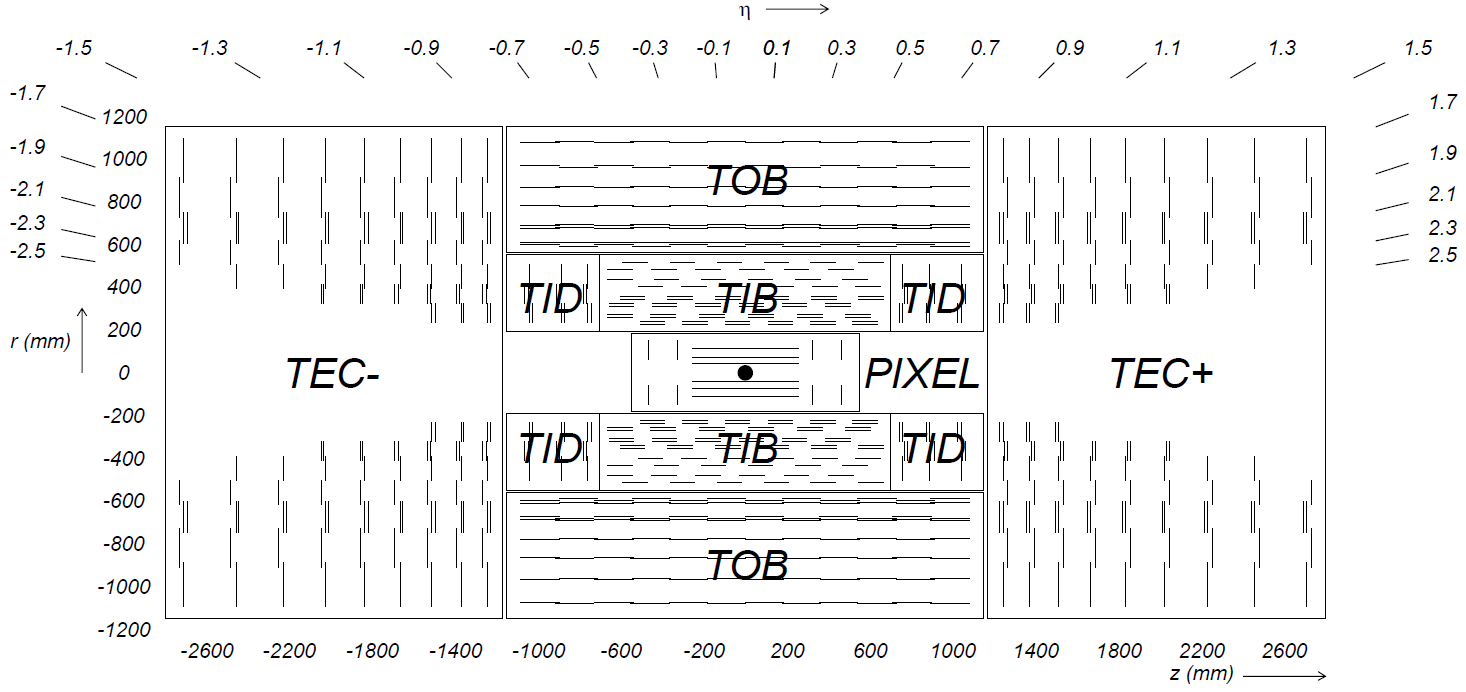
\includegraphics[width=0.9\textwidth]{Figures/CMS_Diagrams/Tracker__Side_View.png}
  \caption{A side view of the tracker.  The pixel detector is the
    innermost sub-system, with three concentric rings of detectors in
    the barrel, and two in the endcap.  The tracker inner barrel (TIB)
  is a silicon strip detector, with four concentrinc rings.  The
  tracker inner disks (TID) are three layers deep.  The tracker outer
  barrel (TOB) is six concentric rings and the tracker end caps (TEC)
  are nine layers deep. } \label{fig:tracker_side}
\end{figure}

\begin{figure}[h]
   \centering
  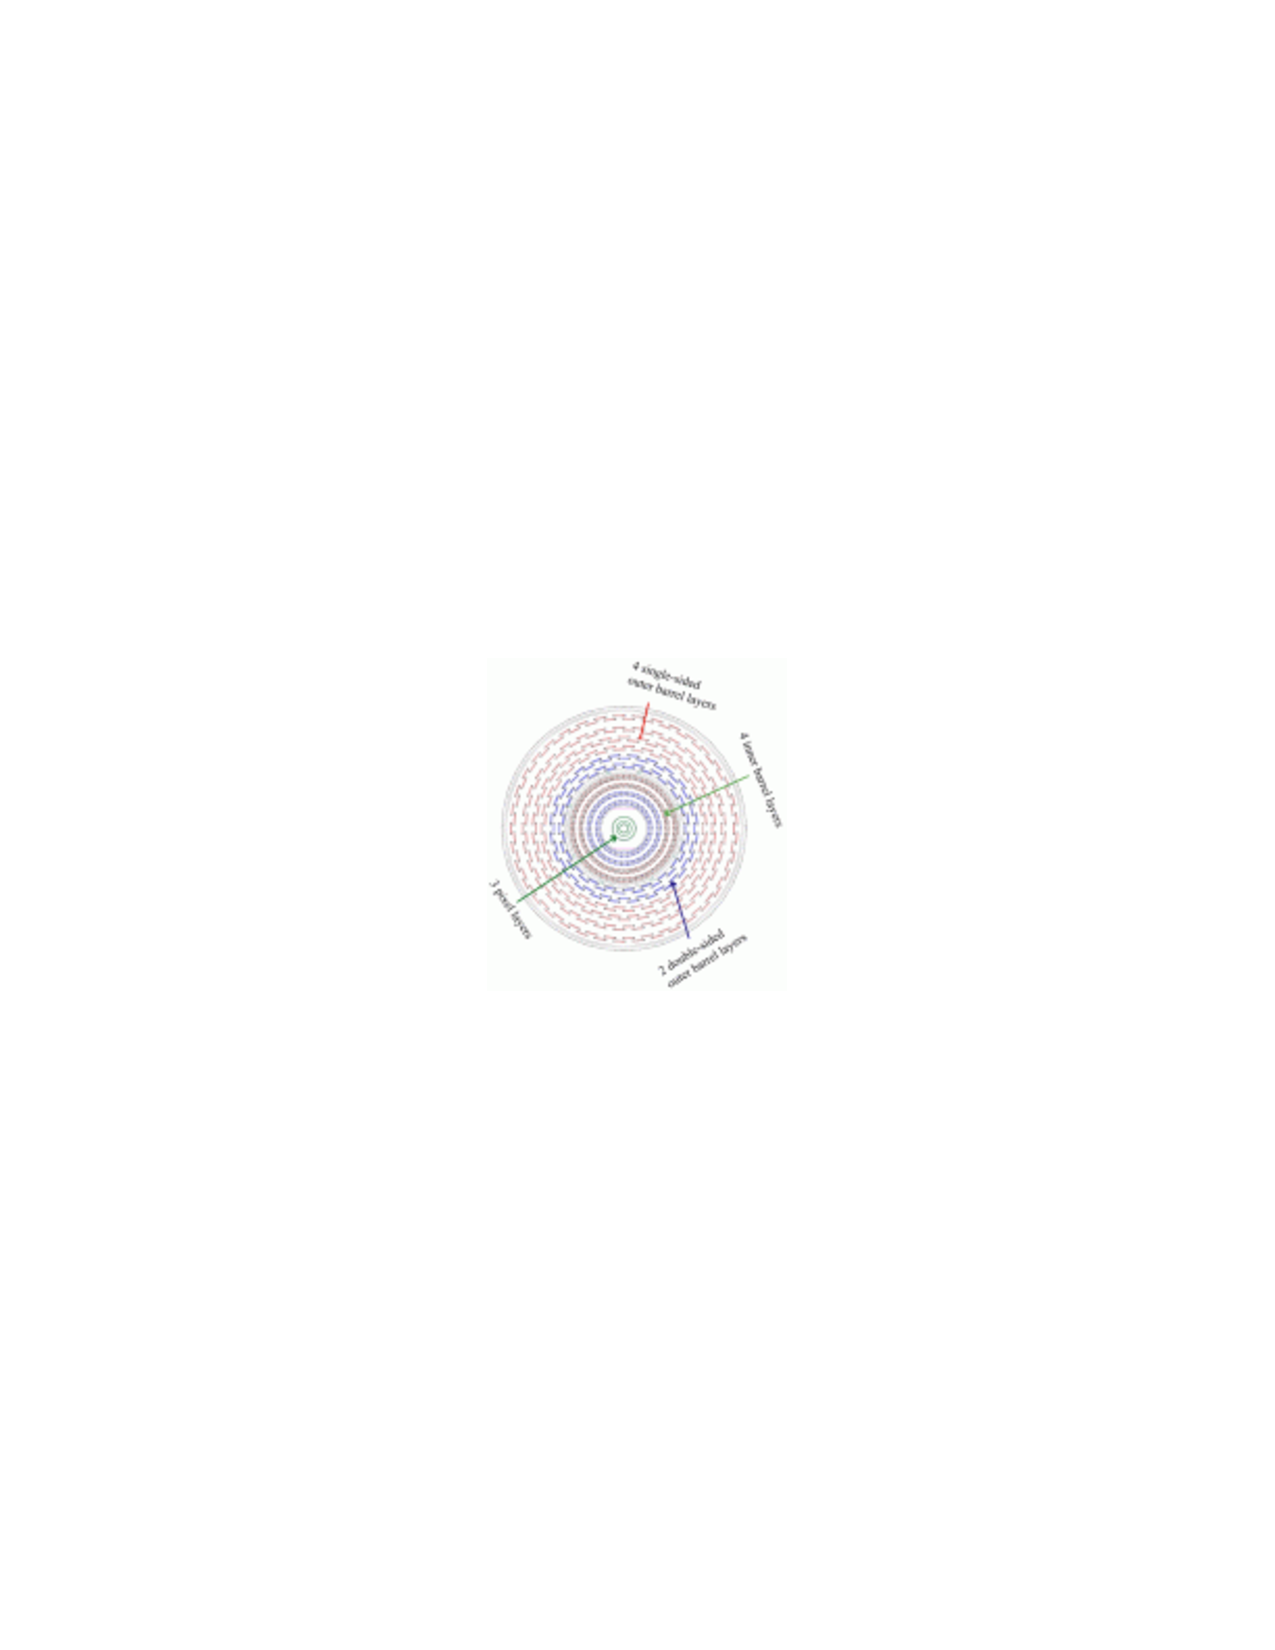
\includegraphics[width=0.5\textwidth]{Figures/CMS_Diagrams/Tracker__Barrel_View.pdf}
  \caption{A head-on view of the beamline and barrel components of the
  tracker.} \label{fig:tracker_barrel}
\end{figure}

\par The tracker has a cylindrical shape that surrounds the interaction 
region, with a length of 5.8 m and a diameter of 2.5 m.  The large
particle flux close to the beamline requires the use of a pixel
detector sub-system in the innermost region, from radius 4.4 cm to
10.2 cm from the beamline.  The particle flux drops off suffciently at
larger radii to use silicon strip dectors, arranged into four
different sub-systems: the tracker inner barrel (TIB), tracker inner
disks (TID), tracker outer barrel (TOB) and tracker end caps (TEC),
which extend to a radius of 1.2 m from the beamline.  Figure
\ref{fig:tracker_side} shows a side view of the tracker layout and
figure \ref{fig:tracker_barrel} shows a view down the beamline of the
barrel sections.  The tracker has a total acceptance of $|\eta|<2.5$.  

\par There are competing factors for the radial length of the
tracker.  More layers allow for more samples of a particle's
trajectory, giving a higher spatial precision, but more material means
photons and hadrons are more likely to decay, and create a shower of
particles that would better measurered through the absorbtion of
energy via caliorimeters. The depth of the tracker varies from 0.4 to
1.8 radiation lengths, resulting in small degration of the ECAL
performance, since approximately half the photons will be converted to
e$^{+}$e$^{-}$ pairs.   

\subsection{The Silicon Pixel Detector}
\label{tracker_pixel_description}

\begin{figure}[h]
   \centering
  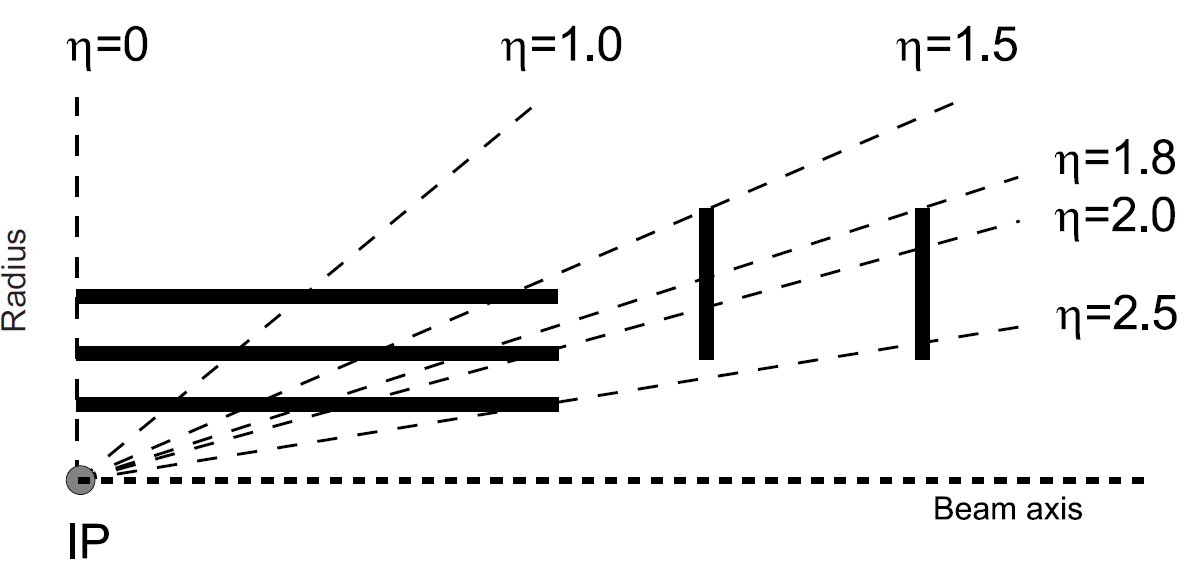
\includegraphics[width=0.8\textwidth]{Figures/CMS_Diagrams/Tracker__Pixel_Rapidity.png}
  \caption{The three barrel and two disk layers of the silicon pixel
    tracker provide coverage of $|\eta|<2.5$ } \label{fig:tracker_pixel_eta_coverage}
\end{figure}

\par The pixel detector consists of 66 million 100$\times$150 $\mu$m
pixels, arranged in three concentric cylindrical layers of radius of
4.4, 7.3, and 10.2 cm from the beam line and two disc layers on either
side of the barrel detectors.  Figure
\ref{fig:tracker_pixel_eta_coverage} shows the eta coverage of the
detector out to $|\eta|<2.5$.   

\par The sensor technology uses a $n$-on-$n$ concept, where a
high-dose $n$-implant is introduced onto a $n$-substrate with large
resistance.  A $p-n$ junction is made by the placement of a $p$-type
semiconductor on the back side of the substrate.  When a charged
particle passes through the face of the substrate, between the $p-n$
junction, it liberates electrons from the silicon atoms, creating 
electron-hole pairs.  The $p$-side has a voltage bias of 150 V in the
barrel, and 300 V in the disks, that sweeps the pair apart, creating a
current.  Pixels are isolated from one another using a moderated
$p$-spray in the barrel region, and open $p$-stops in the disks in
order to create an additional $p-n$ structure that acts like a diode
to limit current flow between pixels.  The 3.7 T magnetic
field of the CMS solenoid also induces a Lorentz drift of the current
in the $\hat{\phi}$ direction.  This results in the current produced
in one pixel being shared among multiple neighboring pixels.  The
charge collected by each of the multiple pixels are read-out, using an
interpolation between pixels, resulting in a 15-20 $\mu$m spatial resolution
on the trajectory of the charged particle - much smaller than the size
of an individual pixel.  In order to induce this effect in the disks
(where the pixels are orientated perpendicular to the barrel), the
pixels are angled 20$^{\circ}$ in the $\hat{y}$ direction. 

\begin{figure}[h]
   \centering
  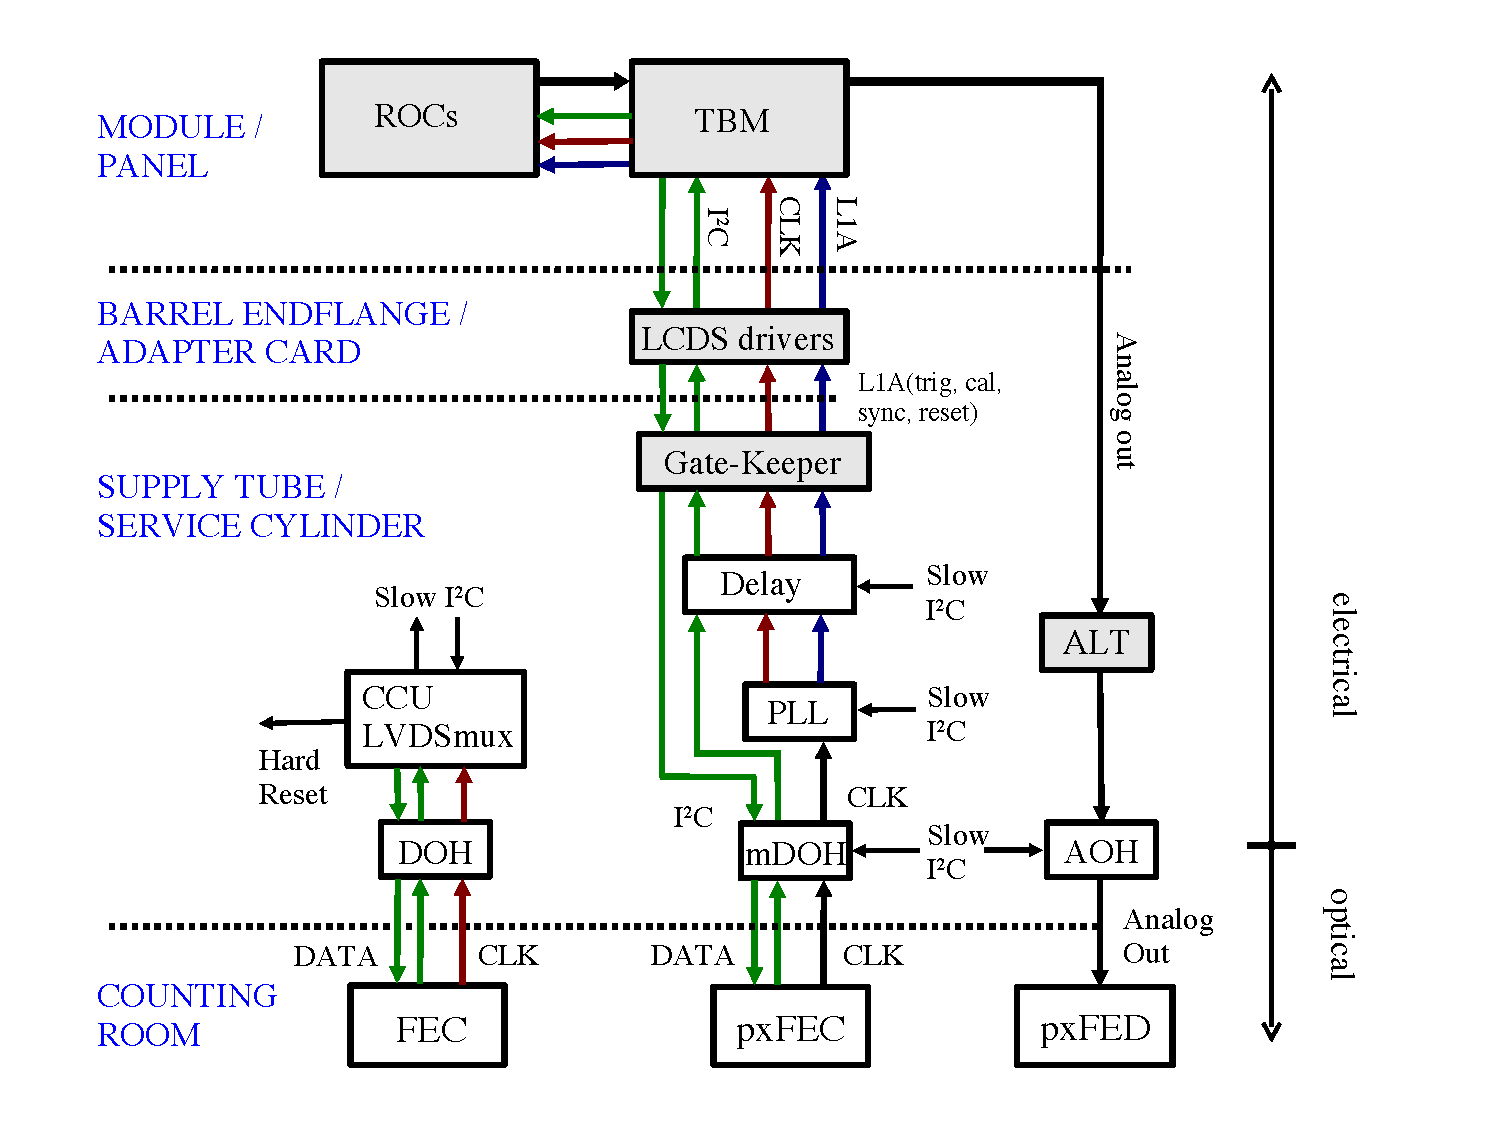
\includegraphics[width=0.8\textwidth]{Figures/CMS_Diagrams/Tracker__Pixel_Readout.pdf}
  \caption{The readout electronics chain for the pixel detector} \label{fig:tracker_pixel_readout}
\end{figure}


\par The current created by the charged particle is collected by a
readout chip (ROC) that is soldered with a bump bond type connection
to the pixel.  The ROC is a custom ASIC chip, that processes the
signals for a grid of 52x80 pixels.  It provides amplification,
buffering, and zero suppresion (threshold) of the charge from each
pixel.  Depending on the layer, 8-16 ROCs in the barrel, and 21-24 ROCs in
the disks are connected and read-out by a single token bit manager
(TBM) chip.  This chip communicates information from the sensors to
the trigger system, which is used to determine whether a given event
is stored as data for analysis later.  The pixel front end controller
(pxFEC) interfaces with the ROC and TBM and provides central clocking
and communicates to the CMS data acquisition system.  The pixel front
end digitizer (pxFED) converts the analog signals from the ROC and
TBMs.  A total of 40 pxFED (32 in the barrel and 8 in the disks)
modules are used to read-out the entire pixel detector, and figure
\ref{fig:tracker_pixel_readout} shows a schematic of the pixel
read-out chain. 

\begin{figure}[h]
   \centering
  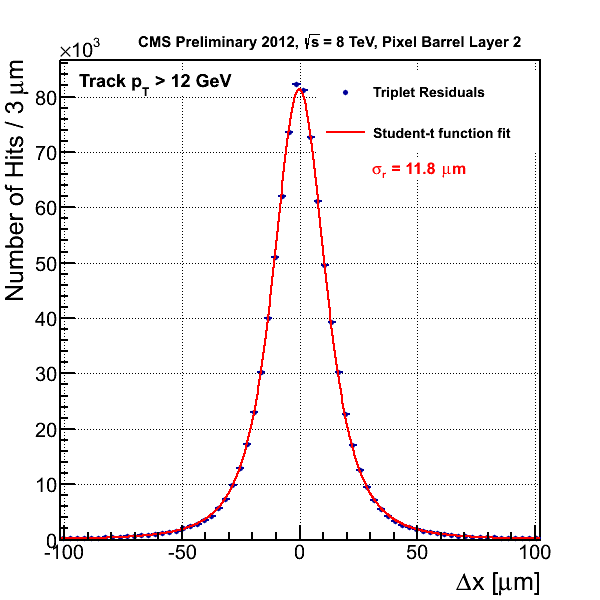
\includegraphics[width=0.8\textwidth]{Figures/CMS_Diagrams/Tracker__Pixel_Resolution__2012_data.png}
  \caption{In 2012 $pp$ collisions at $\sqrt{s}=8 \TeV$, the pixel
    detector performed wiht a resolution of 11.8 $\mu$m.  The above
    is a plot of the residual difference between a pixel and the
    results of a fit to a particle track.} \label{fig:tracker_pixel_resolution}
\end{figure}

\par The resolution of the pixel detector was measured in 2012 with
$\sqrt{s}=8 \TeV$ $pp$ collision.  The residual distance between the
hit position recorded by a pixel, and an interpolated track that uses
that hit is plotted and fit with a student-t function in figure
\ref{fig:tracker_pixel_resolution}.  For tracks with \PT$>$12 \GeV, the
pixel detector was found to have a spatial resolution of 11.8 $\mu$m. 


\subsection{The Silicon Strip Detector}
\label{tracker_strip_description}

\begin{figure}[h]
   \centering
  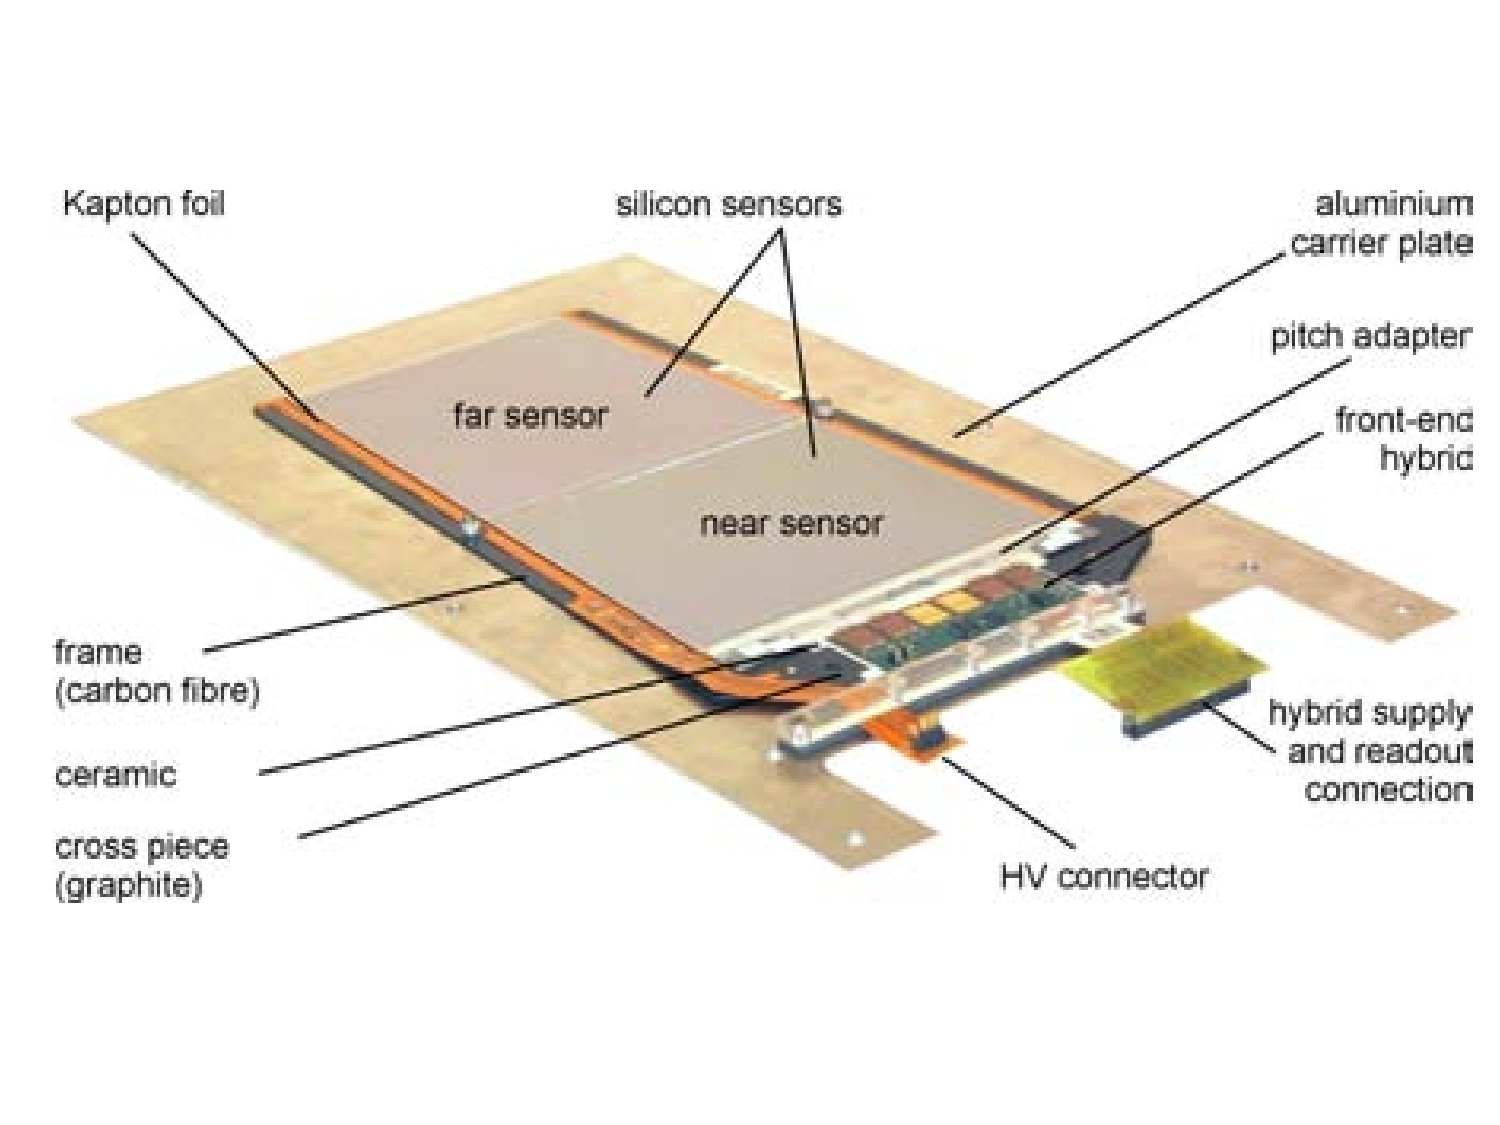
\includegraphics[width=0.7\textwidth]{Figures/CMS_Diagrams/Tracker__Silicon_Strip_Module.pdf}
  \caption{A silicon strip module, with two 500 $\mu$m thick sensors.} \label{fig:tracker_strip_module}
\end{figure}

\par As shown in figure \ref{fig:tracker_side}, the silicon strip
tracking system has four components: the tracker inner barrel (TIB),
tracker inner disks (TID), tracker outer barrel (TOB) and tracker end
caps (TEC).  A total of 15,148 detector modules are distributed among
these systems, each with either one 320 $\mu$m thick sensor, or two
500 $\mu$m thick sensors, making 24,244 sensors with an active area of
198 m$^{2}$ of silicon.  A modele with two sensors is shown in figure
\ref{fig:tracker_strip_module}.  Each sensor has either 512 or 768 strips
since they are read out by two multiplexed 128-channel front end
chips, making it possible to only read out sensors in groups of 256.
Each strip has a pitch that varies between 80 and 200 $\mu$m and
lengths that vary between 10 and 25 cm.  All in all, 9.3 million
strips are used in the silicon tracker.  

\par The TIB and TID provide radial coverage from 20 to 55 cm.  The
TIB has four barrel layers, with 80 $\mu$m pitch strips on the first two
layers, and 120 $\mu$m strips on the outer two, giving a single point
resolution of 23 and 35 $\mu$m repsectively.  The strip pitch varies
between 100 and 141 $\mu$m in the three discs of the TID.  The TOB
surrounds the TIB/TID and is composed of six barrel layers that extend
the tracker raidus to 116 cm.  It is composed of 500 $\mu$m thick
strip sensors, with pitches of 183 $\mu$m in the first four layers and
122 $\mu$m in the outer two layers.  It provides 6 measurement points
of the particle trajetory with a single point resolution of 53 (35)
$\mu$m in the first four (last two) layers.  Each TEC is made of 9
discs, each with 7 rings of strip detectors.  The inner four rings of
each disk use the single, 320 $\mu$m thick strip modules, while the
outer three rings use the double, 520 $\mu$m thick strip modules.  The
average pitch varies between 97 to 184 $\mu$m in each of the rings.
In the first two layers of the TIB, the first two rings of the TID,
the first two layers of the TOB, and rings 1, 2, and 5 in each disk of
the TEC contain modules mounted back-to-back, with an angle of 100
mrad between them to provide a two-dimensional measurement of a
particle's trajectory.  

\par Each of the strips is a single sided $p$-on-$n$ type silicon
sensor manufactured on 6 inch wafers, with a base material of $n$
doped silicon.  The front side of the wafer is implanted with a
$p^{+}$ type semiconductior.  A uniform $n^{+}$ implantation on the
back forms the ohmic contact to 500 V.  This forms a $pn$ junction and
when a charged particle passes through the face of the wafer, atoms in
the junction are ionized and the 500 V potential difference creates a
current out of the resulting electron/hole pairs.  This current is
collected and processed through the read-out system.  

\begin{figure}[h]
   \centering
  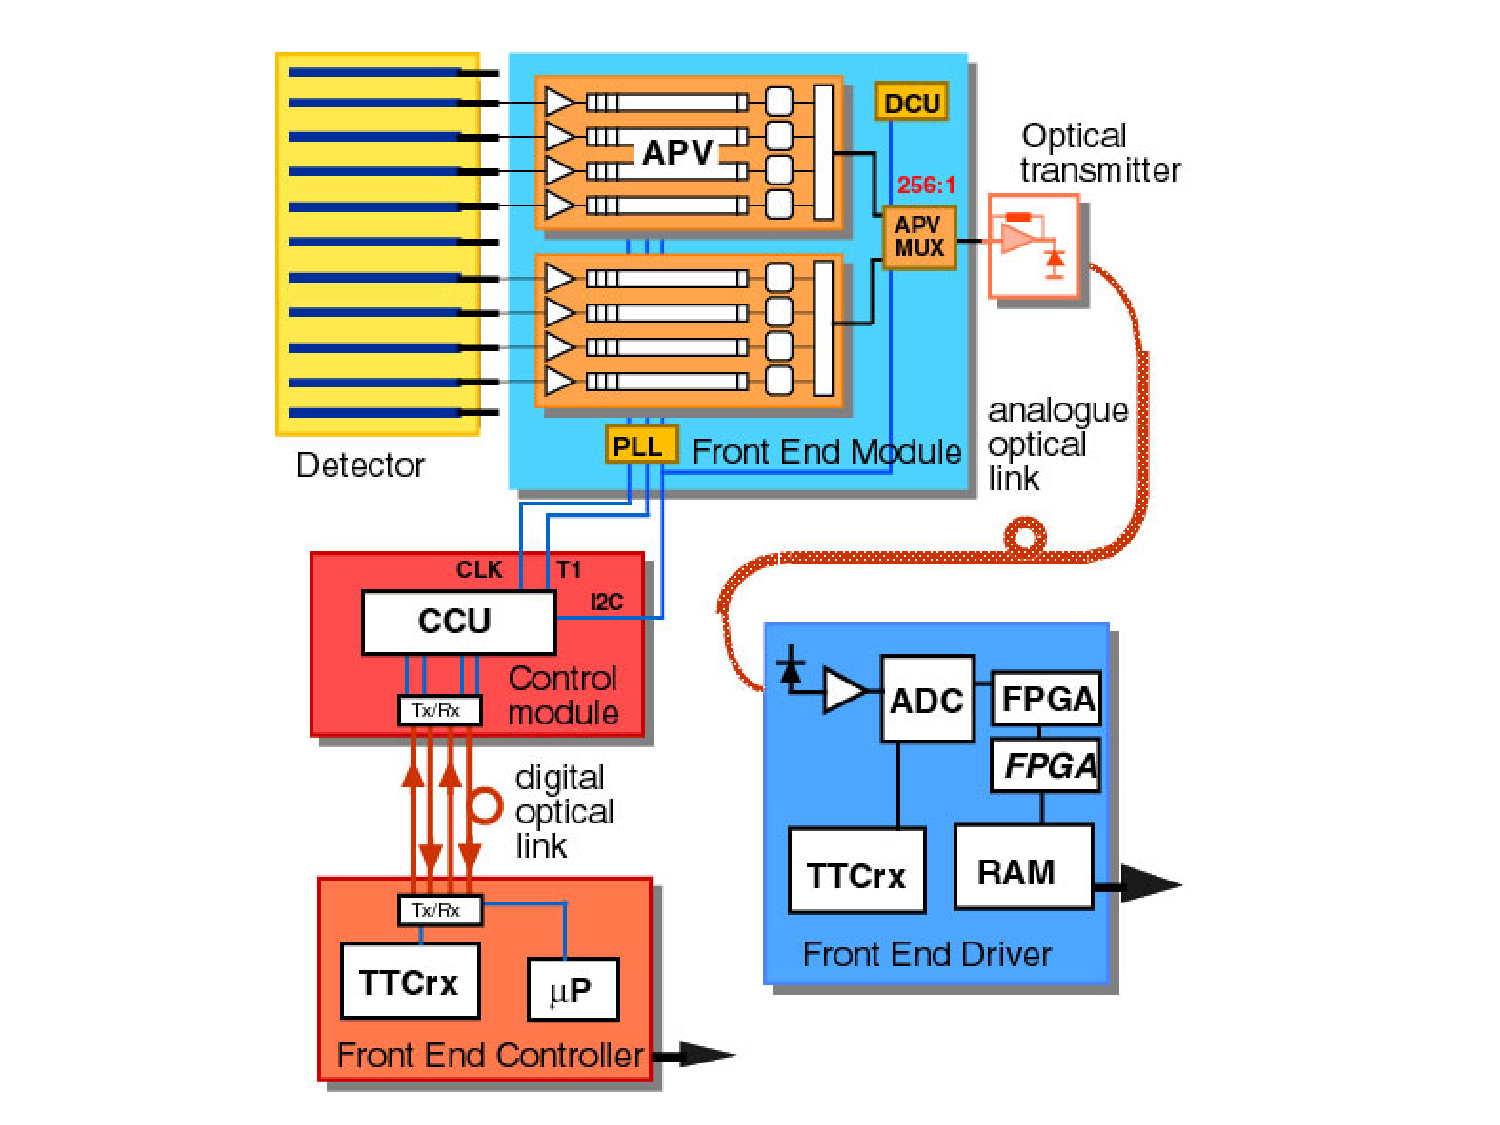
\includegraphics[width=0.7\textwidth]{Figures/CMS_Diagrams/Tracker__Silicon_Strip_Readout.pdf}
  \caption{Schematic of the readout sequence of the silicon strip
    detector.} \label{fig:tracker_strip_readout}
\end{figure}

\par A custom integrated circuit, the APV25, is used to amplify,
shape, and buffer the signals produced from the silicon strips.  It
has 128 read-out channels, and samples the detector signals at the 40
MHz, suitable for the 25 ns collisions.  It is able to store data for
up to 4 $\mu$s to account for trigger latency.  Two APV25 chips are
linked with fiber optics to the Front End Driver (FED) system.  Each
FED receives data from 94 optical fibers, and digitizes them in
parallel.  The Front End Controller (FEC) transmits clock, trigger,
and control data to the APV25s.  The entire readout chain is shown in
figure \ref{fig:tracker_strip_readout}. 

\begin{figure}{h}
    \centering
    \begin{subfigure}[h]{0.450\textwidth}
        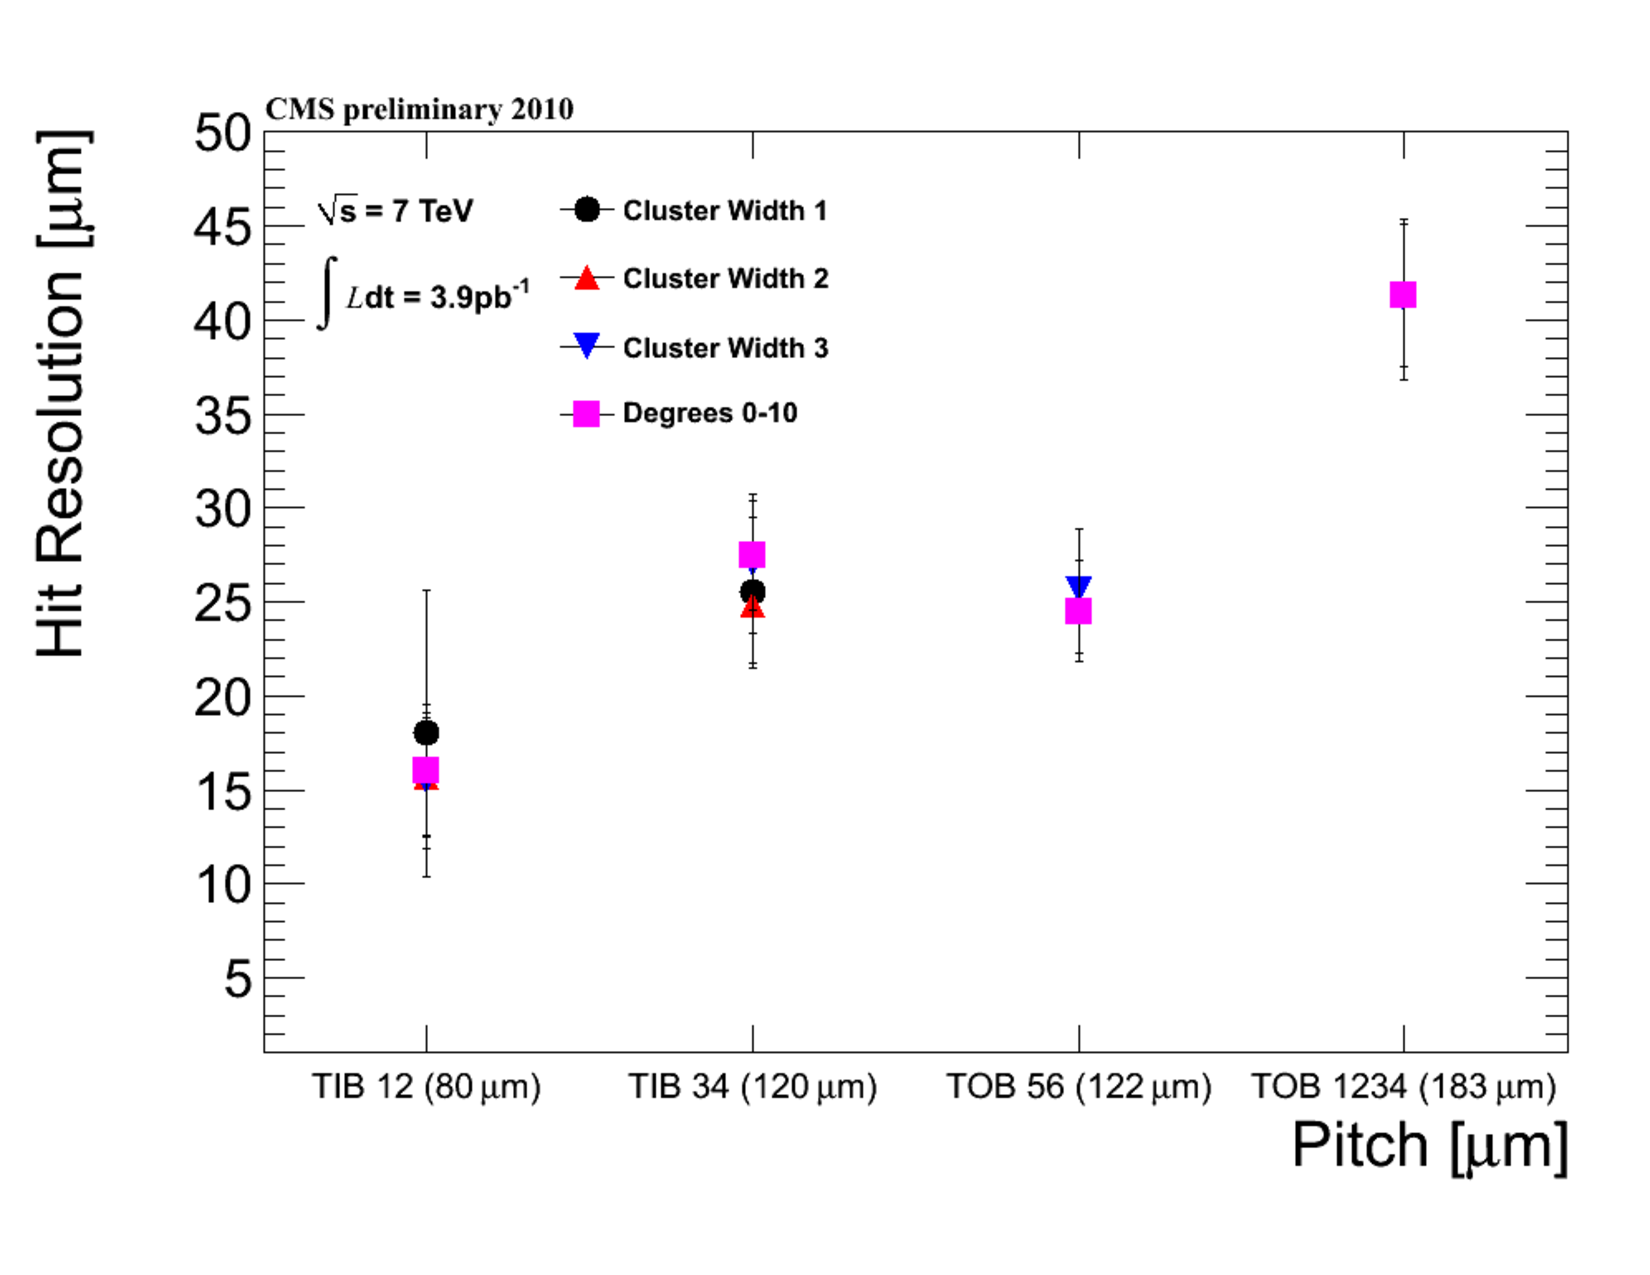
\includegraphics[width=\textwidth]{Figures/CMS_Diagrams/Tracker__Strip_HitRes.pdf}
        \caption{Measurment of the resolution on charged particle
          tracks in the TIB and TOB}\label{fig:tracker_strip_hitRes}
      \end{subfigure}
      ~ %add desired spacing between images, e. g. ~, \quad, \qquad, \hfill etc.
      % (or a blank line to force the subfigure onto a new line)
    \begin{subfigure}[h]{0.450\textwidth}
        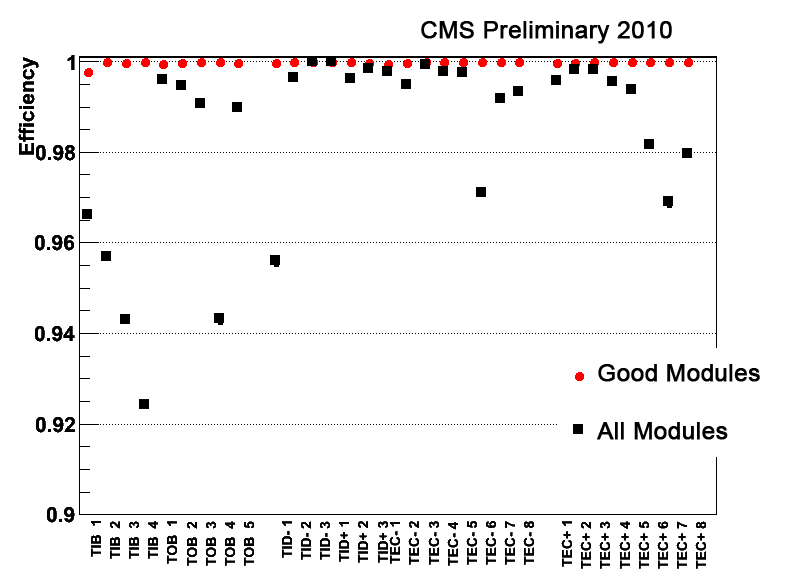
\includegraphics[width=\textwidth]{Figures/CMS_Diagrams/Tracker__Strip_efficiency_end2010.png}
        \caption{Strip tracker efficiency for identifying charged tracks}\label{fig:tracker_strip_efficiency}
      \end{subfigure}
      \caption{Measurements of the performance of the silicon strip
        track using $pp$ collisions from 2011 at $\sqrt{s}=7 \TeV$}\label{fig:tracker_strip_performance}
\end{figure}

\par In 2011, the strip efficiency and resolution were measured from data
in center-of-mass energy, $\sqrt{s}=7 \TeV$ $pp$ collisions.  Figure
\ref{fig:tracker_strip_performance}(\subref{fig:tracker_strip_hitRes})
shows the resolution varying between 15-40 $\mu$m for the TIB and TOB
detectors.  Figure
\ref{fig:tracker_strip_performance}(\subref{fig:tracker_strip_efficiency})
shows the efficiency for reconstructing tracks with the strip tracker,
which is well above 99$\%$ when only considering operational modules.   


\section{The Electromagnetic Calorimeter}
\label{ecal_description}

\begin{figure}[h]
   \centering
  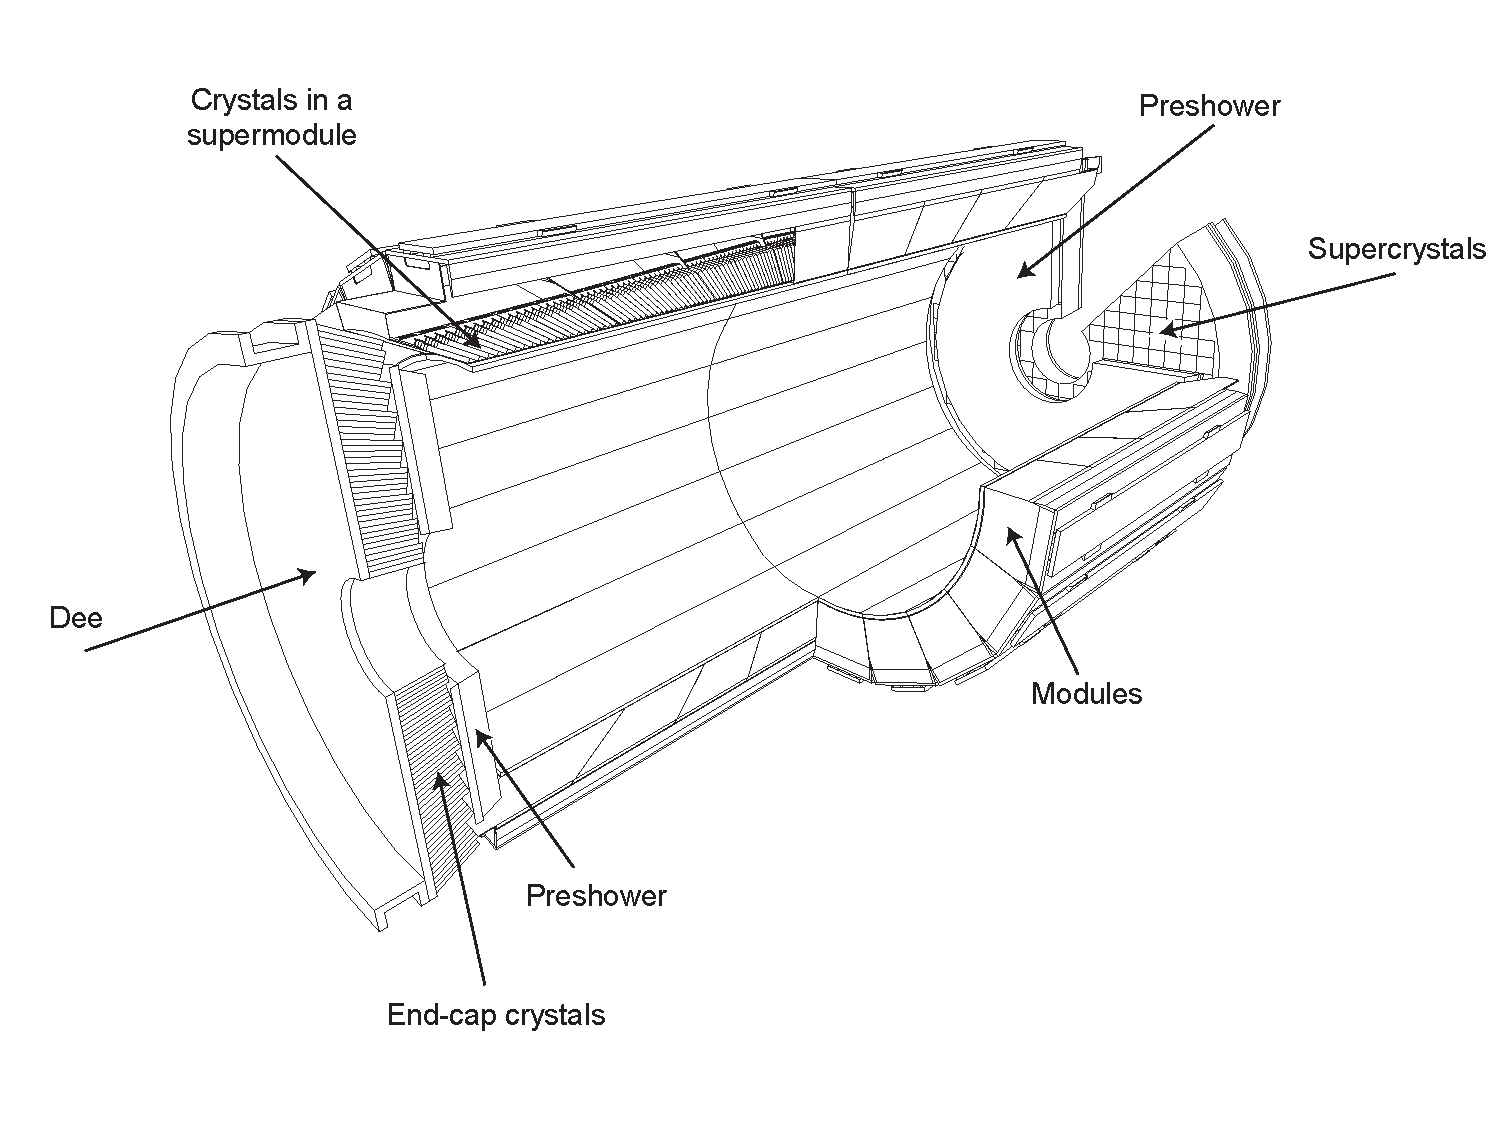
\includegraphics[width=0.7\textwidth]{Figures/CMS_Diagrams/ECAL__Layout.pdf}
  \caption{Layout of the ECAL sub-detector} \label{fig:ecal_layout}
\end{figure}

\par The \acrfull{ecal} surrounds the inner tracker with 61,200 high
density lead tungstate (PbWO$_{4}$) crystals in the central barrel
section, and 7,324 crystals in each of the two endcaps.  The crystals
have a fast response, provide fine granularity, and are radiation
resistant, making them ideal for the LHC environment and the physics
goal of observing the Standard Model Higgs boson decay to two high
energy photons.  The primary background for this process comes
from neutral pions decaying to two photons, which is especially
difficult when the photons are close together and can potentially be
reconstructed as a single high-energy photon.  This occurs most
frequently in the endcaps, so an additional detector, the preshower,
provides additional spatial resolution with silicon microstrip
detectors, similar to those in the tracker. Figure
\ref{fig:ecal_layout} shows the layout of the ECAL.  

\begin{figure}[h]
   \centering
  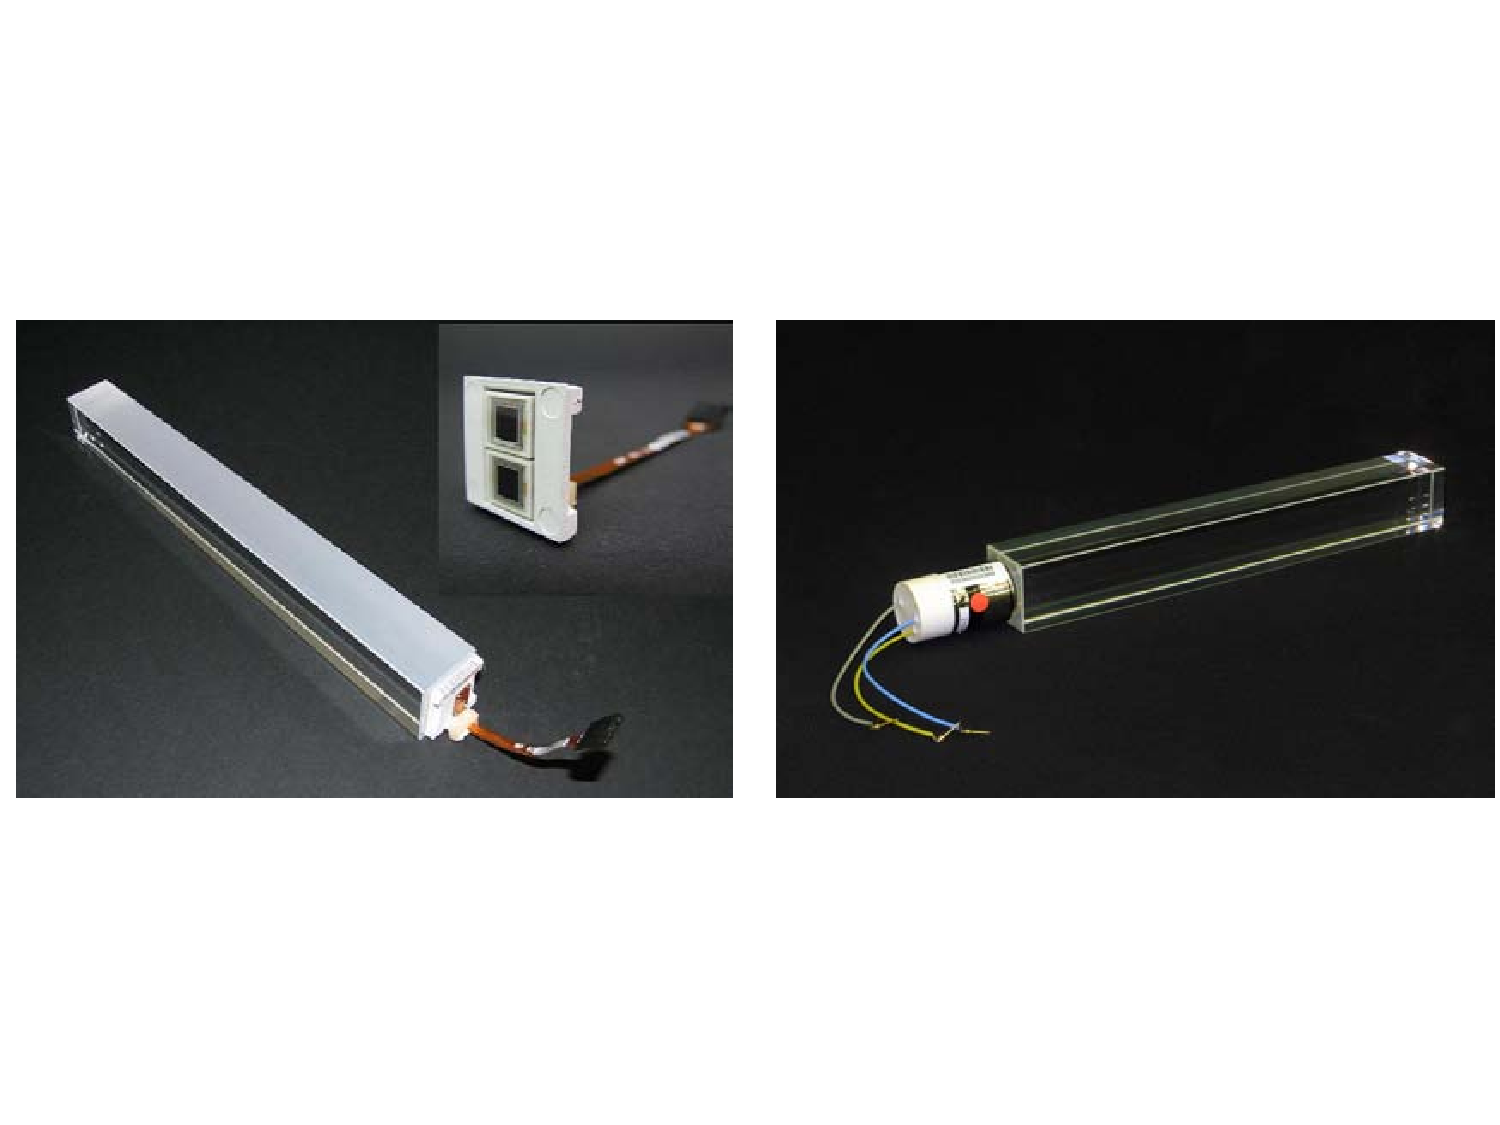
\includegraphics[width=0.9\textwidth]{Figures/CMS_Diagrams/ECAL__Xtal.pdf}
  \caption{Typical Lead Tungstate crystal, with APD attached to the
    rear face in the left frame, and a VPT attached in the right
    frame. } \label{fig:ecal_xtals}
\end{figure}

\par Lead tungstate is in ideal material for electromagnetic
calorimetry.  Figure \ref{fig:ecal_xtals} shows a typical crystal,
with photomultipliers attached to the rear faces, which will be
discussed later.  The material has a high density, 8.28 g/cm$^{3}$, giving it a
large electromagnetic cross-section, making it much more likely for a
particle traversing the crystal to interact with one of the atoms in
its structure.  When a particle interacts with the crystal, it does so
by depositing energy into its atoms, which excite the electrons that
are bound to it.  The atoms then relax by emitting photons, in a
process known as scintiallation and the PbWO$_{4}$ crystals release
80$\%$ of their light in the 25 ns LHC bunch crossing time.  This
light is collected by photomultipliers attached to the rear face of
the crystal and converted into an electrical signal.  Read-out
electronics amplify, digitize, and buffer the signal until it can be
stored as data or discarded.  

\begin{figure}[h]
   \centering
  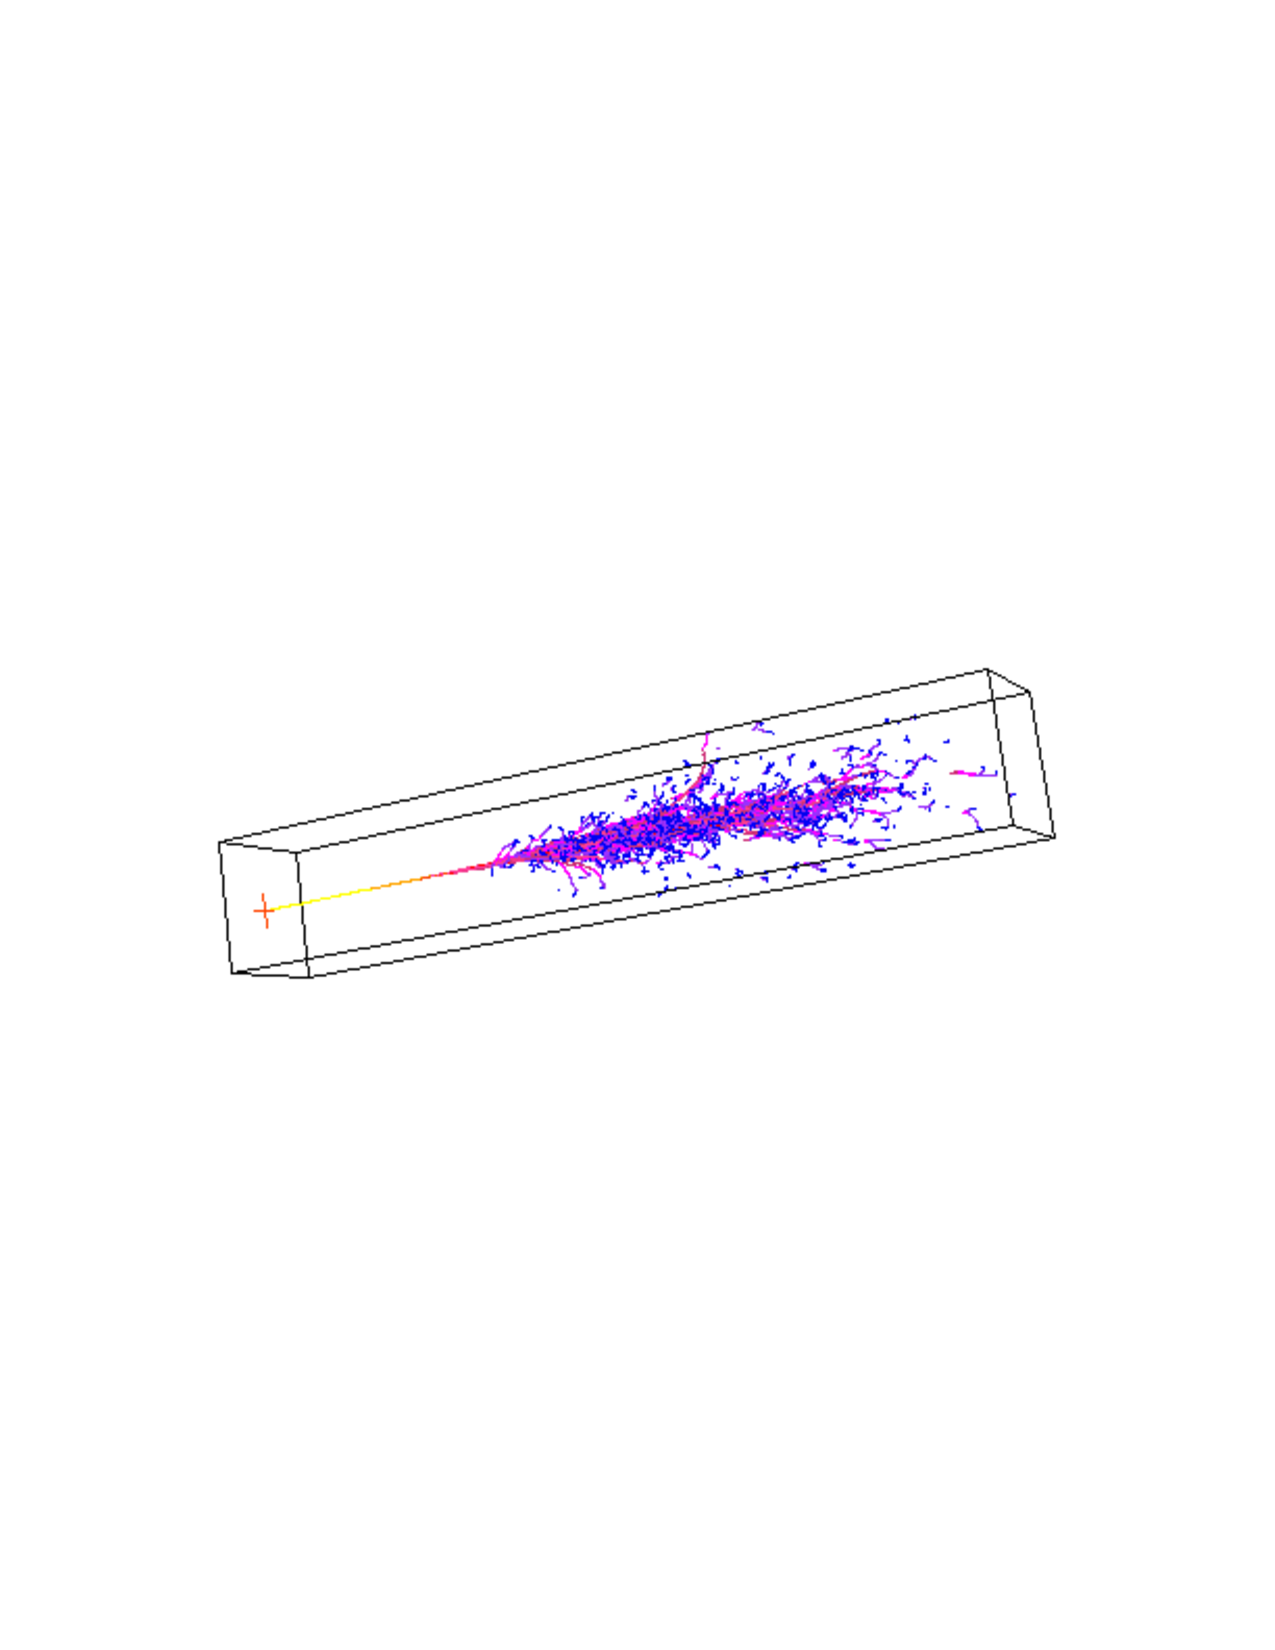
\includegraphics[width=0.7\textwidth]{Figures/CMS_Diagrams/ECAL__shower_simulation.pdf}
  \caption{A simulation of the evolution of a electromagnetic shower
    being initiated by an electron entering the center of the front face. } \label{fig:ecal_shower}
\end{figure}

\par As a charged particle or photon begins to deposit energy, it
begins a decay chain into many lower energy photons and electrons,
known as an electromagnetic shower.  Electrons, being bent by the CMS
magnetic field, and multiple scattering off of the PbWO$_{4}$
crystals, create bremsstrahlung photon radiation.  Since the intensity
of bremsstrahlung is inversely proportional to the mass of the
particle squared, particles heavier than electrons such as muons and
hadrons do lot leave a large signature in the ECAL.  Photons convert
to e$^{+}$e$^{-}$ pairs, which in turn create additional
bremsstrahlung. The crystals have a short radiation length,
X$_{0}$=0.89cm, which is the distance it takes an electron to deposit
1/e of it's energy through bremsstrahlung, and 7/9 of the mean free
path of a high energy photon before it converts to an  e$^{+}$e$^{-}$
pair.  A corrolary of the crystal's short radiation length is its
small Moliere raidus, 2.2cm, which is the radius of a cylinder that
encloses of 90$\%$ of the electromagnetic shower's energy
deposition. A typical crystal has a front face that is 22$\times$22
mm$^{2}$, a rear face of 26$\times$26 mm$^{2}$, and a length of 230
mm, or 25.8 X$_{0}$ radiation lengths.  This means that a relatively
small grid of crystals can be used to fully collect the energy
deposited by a high energy electron or photon.  As previously
mentioned, heavier charged particles will not bremsstrahlung as much
as electrons, and will travel through the entire ECAL, depositing only
a moderate fraction of their energy in the crystals.  Figure
\ref{fig:ecal_shower} shows a simulation of an electromagnetic shower
produced by an electron entering the front face of a crystal.      

\begin{figure}[h]
   \centering
  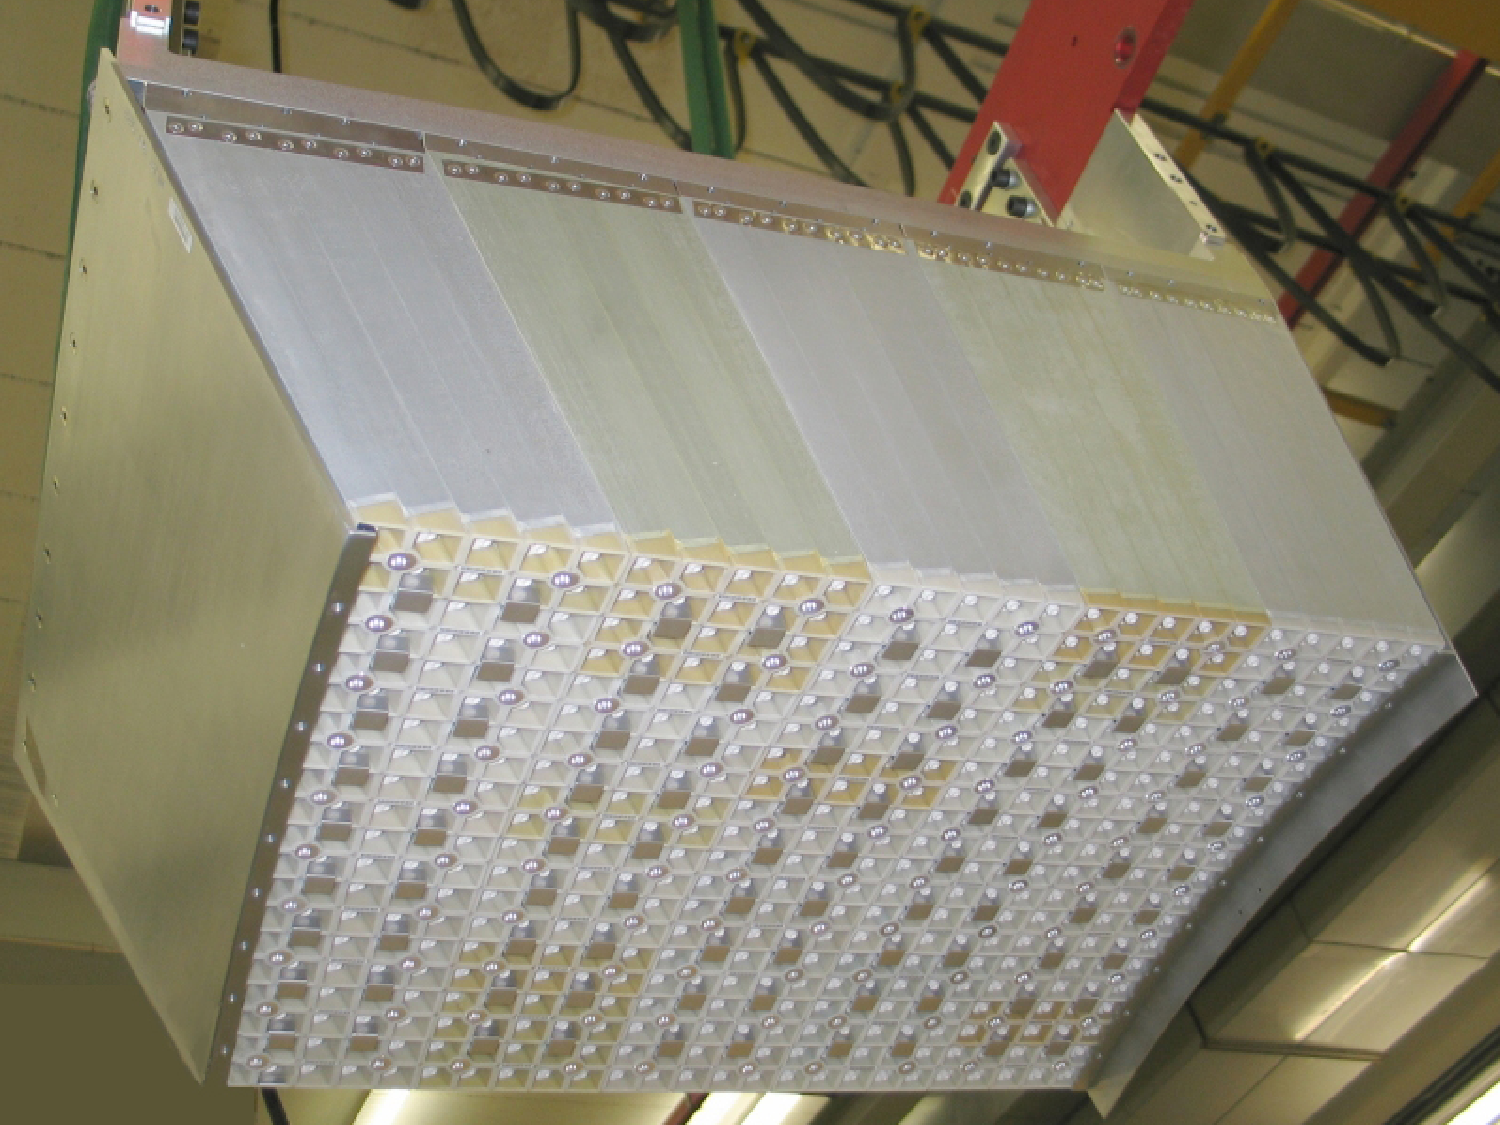
\includegraphics[width=0.7\textwidth]{Figures/CMS_Diagrams/ECAL__Xtal_Module.pdf}
  \caption{A module of 500 crystals (25 crtyals wide by 20 crystal tall). } \label{fig:ecal_xtal_module}
\end{figure}

\par The barrel of ECAL (EB) covers a psuedorapidity range of
$|\eta|<1.479$ with 61,200 crystals at a radius 1.29 m from the
beam-line.  The crytals are positioned in a quasi-projective geometry,
such that their axes make a 3$^{\circ}$ angle with respect to the
vector pointing to the nominal interaction point.  This ensures that
particles will not pass through the cracks and spaces between crytals,
and are forced to interact with a portion of the ECAL. Crystals are
assembled in groups of 400 or 500 into modules, as shown in figure
\ref{fig:ecal_xtal_module} .  Four of these modules are assembled into
a supermodule contain 1700 crystals, and 36 supermodules make up the
barrel region. 

\par The crystals in the EB are read out by Avalanche Photo-Diode (APD)
photomultipliers, shown in the left frame of figure
\ref{fig:ecal_xtals}.  The APDs were manufactured by Hamamatsu and are
a bulk $n$-type silicon material, with a $p$-type implanted on its
surface to form a $pn$-junction.  The operation priniciple is similar
to that of tracker.  When scintilation light from the lead tungstate
crystals enters the face of the APD, it creates electron-hole pairs in
the intrinsic region between the $p$ implantation and the $n$ bulk
material.  The APD is biased with 45 V, which creates a current from
the electron-hole pairs and is the signal that a particle has created
scintilation in the crystal.  The APD provides a gain of 50 and has a
quantum efficiency of 75$\%$.  Both the APDs and the PbWO$_{4}$
exhibit a storng temperature dependence, so the entire system is kept
at 18$^{\circ}$ C with a water-based cooling system distributed
throughout the barrel and end-caps.  

\begin{figure}[h]
   \centering
  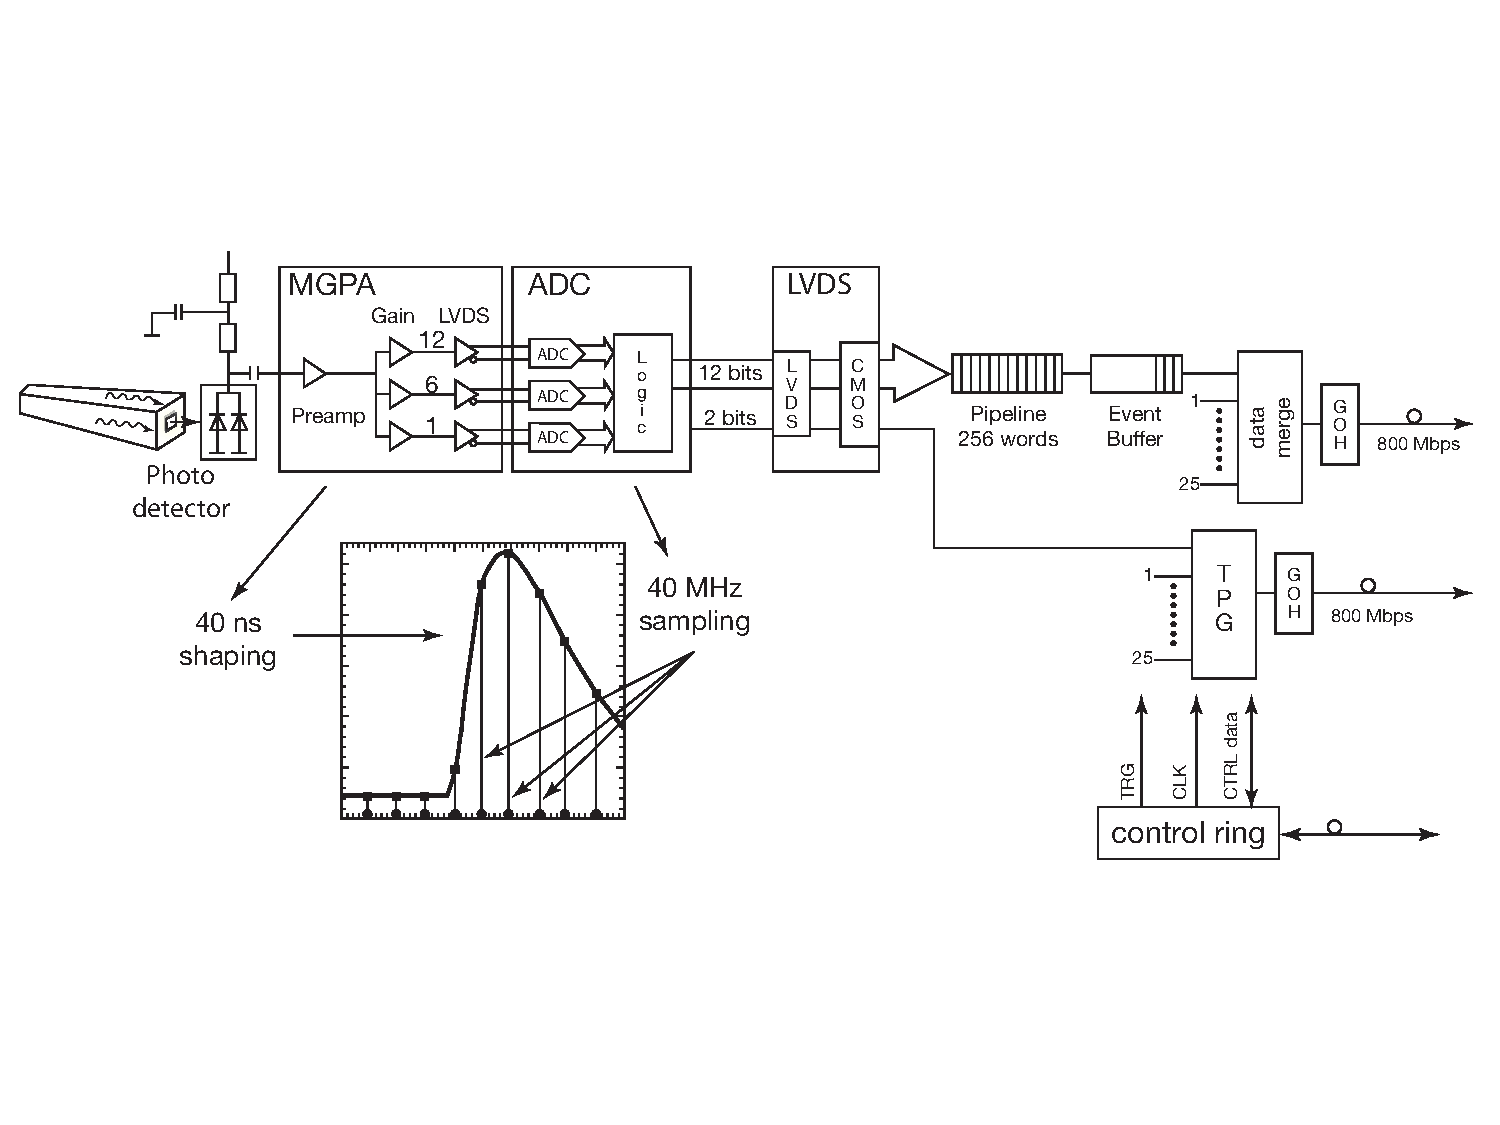
\includegraphics[width=0.75\textwidth]{Figures/CMS_Diagrams/ECAL__OnDetectorReadOut.pdf}
  \caption{Schematic of the On-Detector Readout for the ECAL } \label{fig:ecal_readout}
\end{figure}

\par The ECAL readout elecronics are designed to read-out a 5$\times$5
array of crystals, known as a trigger tower, in the EB, and a single
supercrystal in the EE.  Each trigger or tower or supercrystal
consists of 5 Very Front End (VFE) boards, each connected to 5 APDs
(VPTs), one Front End (FE) board, two (EB) or six (EE) Gigabit Optical
Hybrids (GOHs), one Low Voltage Regulator (LVR) and a motherboard.
Once triggered, the APD (or VPT in the EE) is sampled 10 times, at a
40 MHz sampling rate, and amplified by a multi-gain amplifier (MGPA),
with nominal gains of 1, 6, and 12 contained on the VFE.  These
digitized samples are sent to the FE, where they are buffered until
receiving a Level-1 trigger, where they are sent to the off-detector
elcectronics Data Concentrator Card (DCC) via the GOHs.  Figure
\ref{fig:ecal_readout} shows a schematic of the on-detector read-out. 

\par In the barrel, the 5$\times$5 trigger towers are divided in the 5
stips in the $\hat{\phi}$ direction.  The energy deposits in these
strips is summed by the FE cards and define the transvere energy of
the tower.  In the endcaps, supercrystals are divided into groups of
five contiguous crystals of variable shape, known as
psuedo-strips. The energy of these strips is performed by the FE, and
the off-detector electronics use these to compute the transvere energy
deposition.  

\par The preshower detector sits in front of the ECAL end-caps and
provides coverage from $1.653<|\eta|<2.6$.  It is a two-layer sampling
calorimeter.  Lead radiators initiate electromagnetic showers from
electrons and photons, and silicon strips are placed behind them to
measure trajectories and deposited energy of passing particles.  The
total thickness is 20cm, which corresponds to a 2 raidation lengths in
the first layer, and another radiation length in the second layer.
95$\%$ of photons  are converted to e$^{+}$e$^{-}$ pairs after the
first layer.  Each silicon sensor is composed of 31 strips, with
thickness of 320 $\mu$m and are 1.9 mm in pitch.  A front-end ASIC
performs pre-amplification, shaping, voltage sampling, and
communicates informaiton to the trigger system to determine if data is
stored or discarded.  The structure is formed into Dees, and two Dees
form a disk with a hole for the beam-line to pass through.    

\begin{figure}[h]
   \centering
  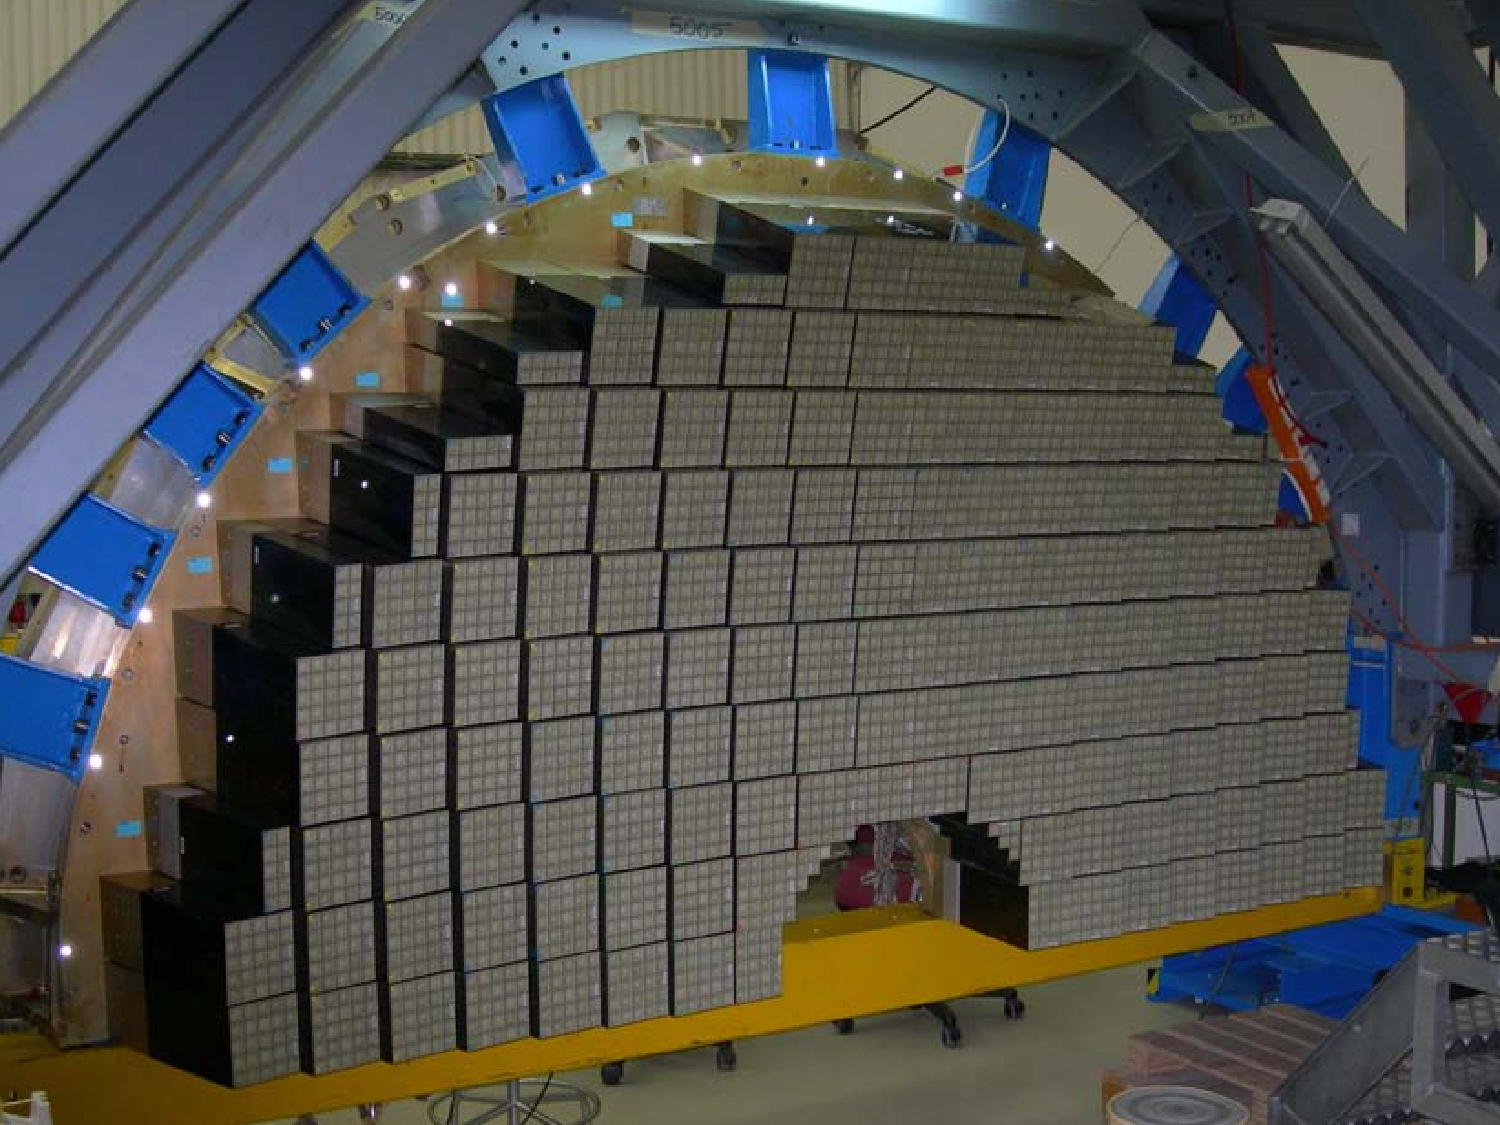
\includegraphics[width=0.7\textwidth]{Figures/CMS_Diagrams/ECAL__EndCap_Dee.pdf}
  \caption{A section of the ECAL end-cap, a Dee.  Two Dees form a disk
  with an inner bore for the beam-line to pass through.  5x5 modules,
  or supercrystals, are mounted in preparation for installation at CMS} \label{fig:ecal_endcap_dee}
\end{figure}

\par Behind the preshower is the ECAL end-cap (EE).  It covers the
psuedorapidity range of $1.479<|\eta|<3.0$, and sits a longitudinal
distance of 315.4 cm from the nominal interaction point.  Crystals are
grouped into 5$\times$5 modules known as supercrystals (SCs).  Like
the preshower, each endcap is divided into two sections, Dees, which
form a disk with an inner bore for the beam line to pass through, as
shown in figure \ref{fig:ecal_endcap_dee}.  Each Dee holds 3,662
crystals, which are divided into 138 supercrysals, and 18 special
partial-supercrystals for the inner and outer sections of the Dee.  

\subsection{Vacuum Photo-Triodes}
\label{vpt_description}

\begin{figure}{h}
    \centering
    \begin{subfigure}[h]{0.450\textwidth}
        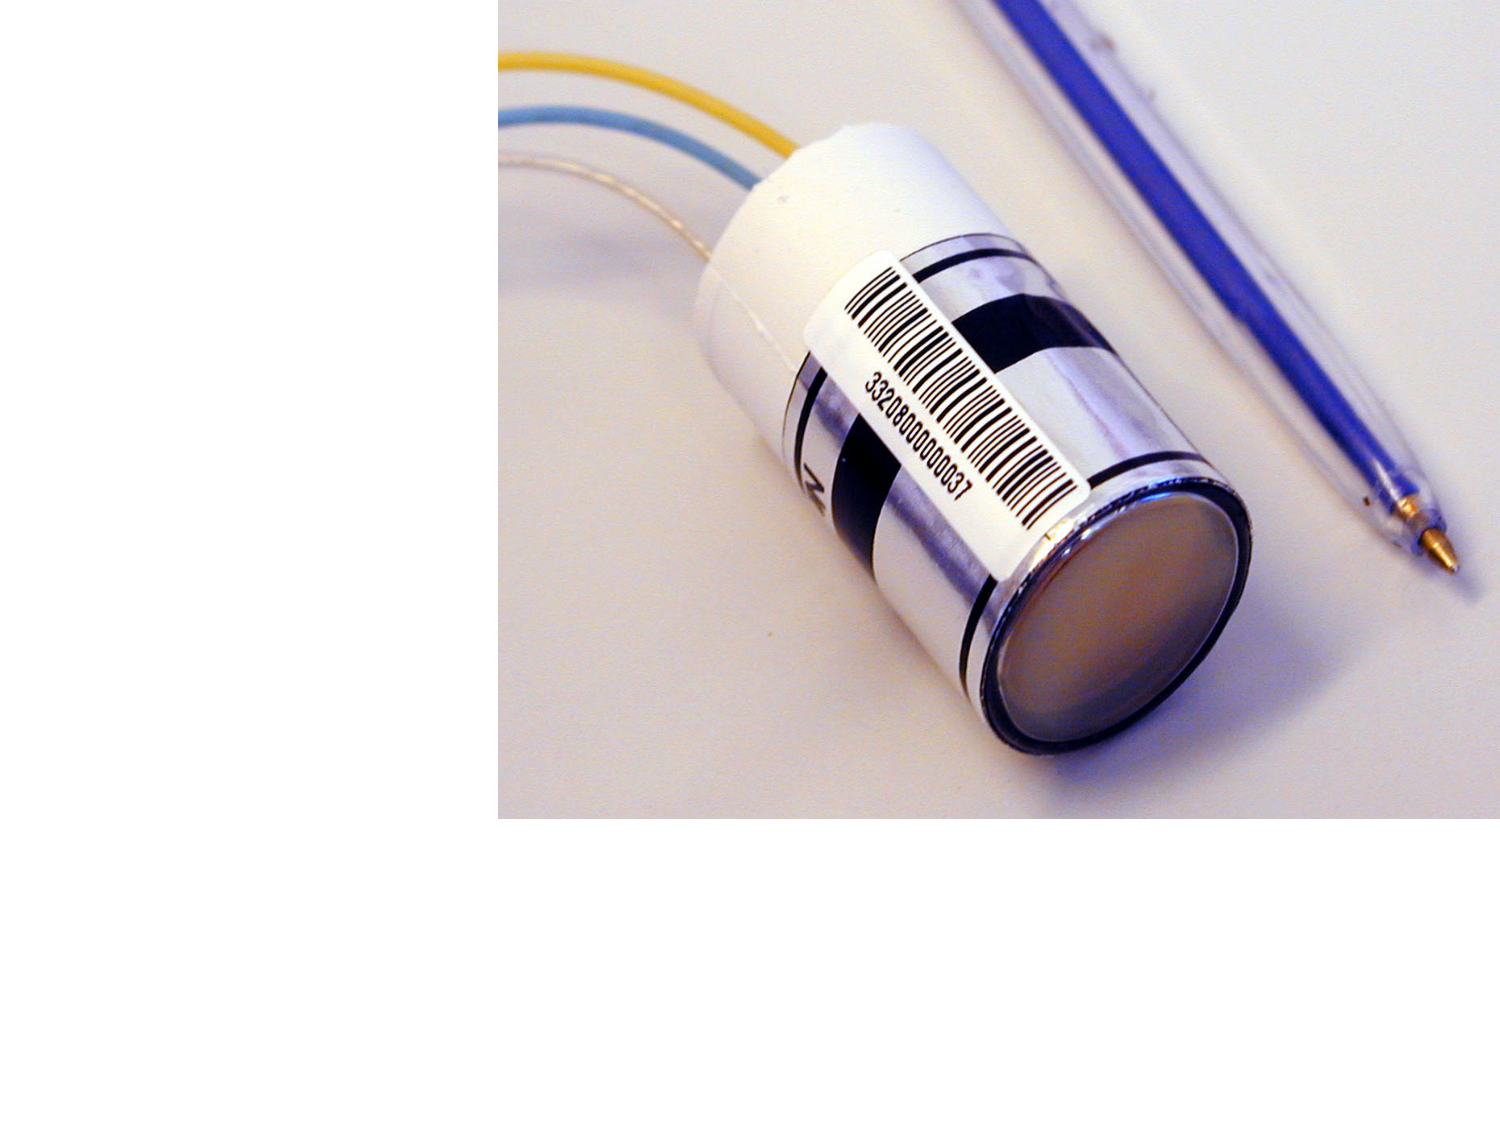
\includegraphics[width=\textwidth]{Figures/CMS_Diagrams/ECAL__VPT.pdf}
        \caption{A picture of a VPT next to a standard size pen for scale}\label{fig:ecal_vpt_pic}
      \end{subfigure}
      ~ %add desired spacing between images, e. g. ~, \quad, \qquad, \hfill etc.
      % (or a blank line to force the subfigure onto a new line)
    \begin{subfigure}[h]{0.450\textwidth}
        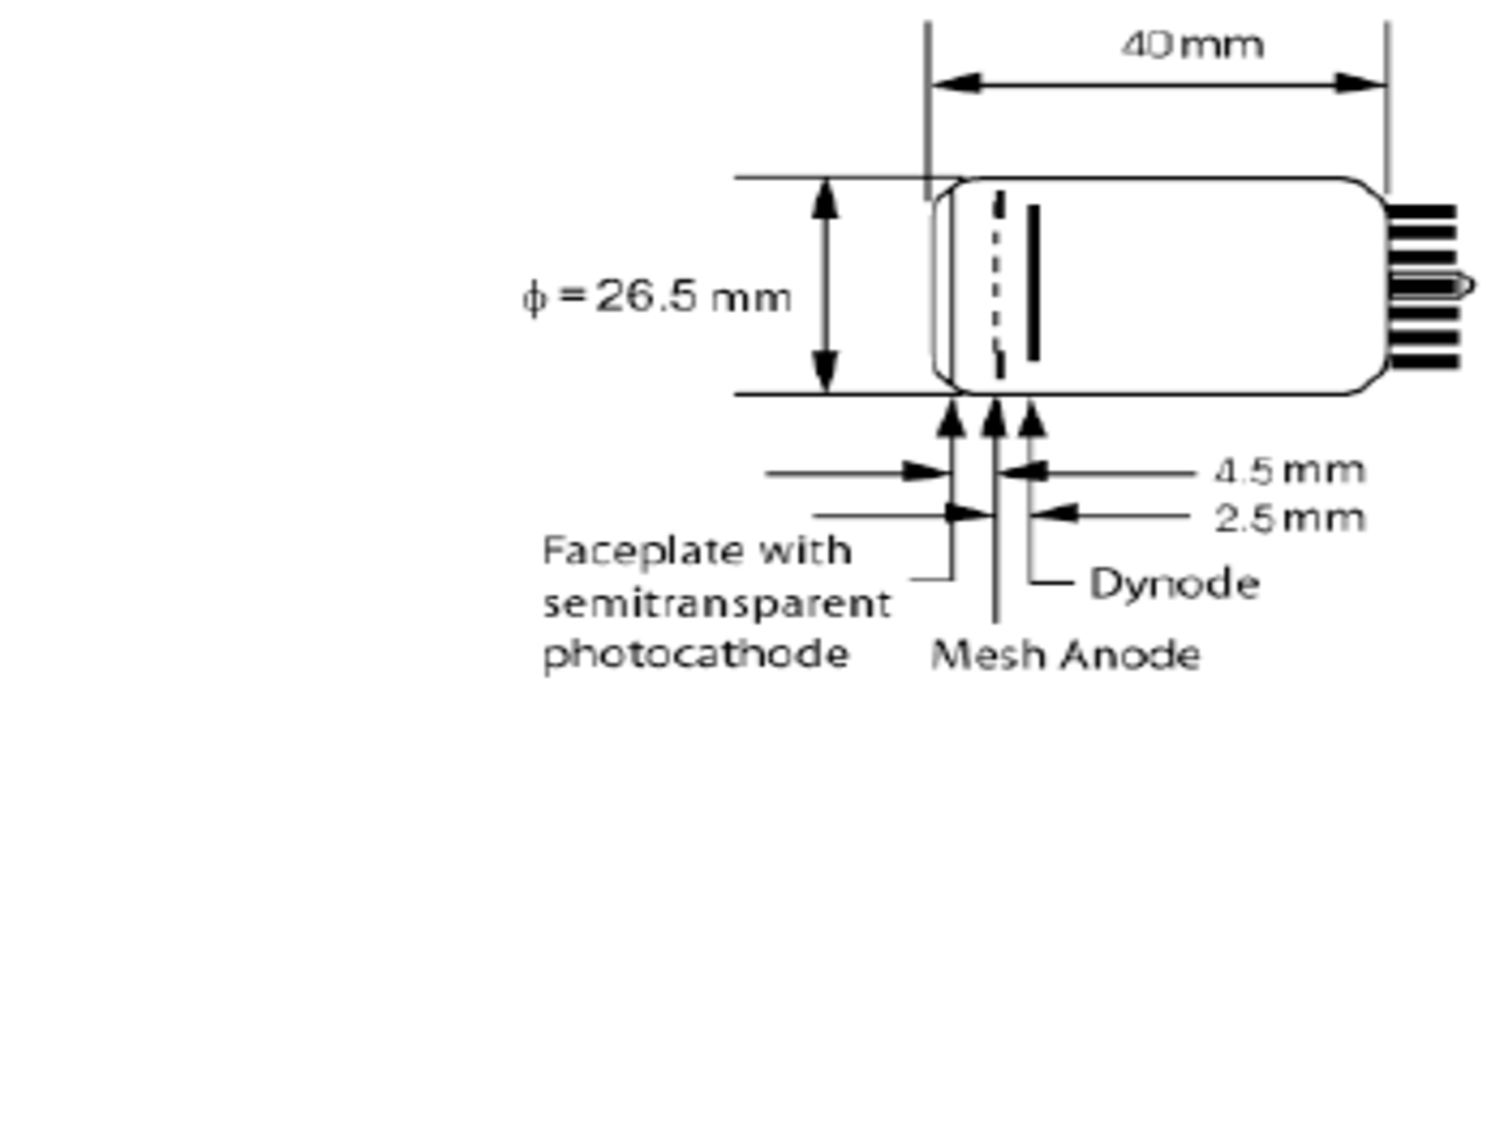
\includegraphics[width=\textwidth]{Figures/CMS_Diagrams/ECAL__VPT_schematic.pdf}
        \caption{Schematic of a VPT showing charcteristic dimensions}\label{fig:ecal_vpt_schematic}
      \end{subfigure}
      \caption{Vacuum Photo-Triode devices used in the ECAL end-caps (EE)}\label{fig:ecal_vpt}
\end{figure}

\par The photomultier used to readout the lead tungstate crystals in
the EE is the Vaccum Photo-Triode (VPT), shown in the right frame of
figure \ref{fig:ecal_vpt}(\subref{fig:ecal_vpt_pic}).  Each device is
26.5mm in diameter and 40mm in lenth as shown in figure
\ref{fig:ecal_vpt}(\subref{fig:ecal_vpt_schematic}).  It is a gain
stage device.  Photons from the lead tungstate scintilation light
enter the front face of the VPT and liberate electrons from the
grounded bialkali photocathode (SbKCs) via the photoelectron effect.
The cathode material has a quantum efficiency of $\sim20-25\%$.  The
photo-electrons are accelerated towards the mesh anode grid, which is
held at 800 V.  Approximately half the photo-electrons pass through
the mesh and encounter a dynode plate held at 600 V.  Electrons either
collide with the dynode, liberating secondary electrons from the
collision, or are turned around by the 200 V differenc between anode
an dynode.  Electrons are thus constantly accelerated towards the
anode, and create secondary electrons as they collide with the anode.
The process repeats with the secodnary electrons, creating an
avalanche of charge near the anode.  As these charges eventually
recombine with the anode over the course of a few nanoseconds, the
voltage of anode drops, signaling the device has detected a photon
from the PbWO$_{4}$ crystals.  

\par  The performance of the VPT is degraded over time by two effects
associated with exposure to the scinitallation light from the crystals.
The first is loss of the vacuum inside the tube.  Molecules from the
air become ionized by the large voltages and the positive ions are
accelerated towards the photo-cathode, which is damaged through the
resulting collision.  The second effect is the gradual depletion of
photo-electrons from the bialkili cathode material.  The result is a
decrease in the current, and thus signal, produced by the anode.  Both
of these effects can be effectively modeled as the sum of two falling
exponential functions.  The University of Virginia has studied the
performance of VPTs with respect to their light exposure rates over
the course of several years in order to characterize the device's
response and long-term behavior.   


\subsection{Test Rig at UVa}
\label{vpt_test_rig_description}

\par The University of Virginia (UVa) has continuously monitored four
production VPTs operated at 800 V anode and 600 V dynode, in a 3.8 T
field, at 15$^\circ$ to the tube axis, with photocathode currents of
approximately 10 nA.  This was done to simulate light exposure from
the lead tungstate crystals in the forward regions of the ECAL
end-caps, as well as provide an accelerated simulation of
photocurrents that would be experienced in the larger eta regions.  As
described above, the light exposure is theorized
to be the most significant cause of the loss of response in the VPT,
known as “burn-in”.  The amount of light that the device has been
exposed to is measured in terms of the total number amount of charge
liberated from the cathode, measured from the cathode current draw,
and is known as the integrated charge.  By operating at such high
photocurrents, UVa is able to probe this burn-in effect in an attempt
to understand the long term behaviour of the VPT response to light.  

\par The University of Virginia is well suited to test these devices,
since it operates a 3.8 T solenoid magnet, with a sufficiently large
inner bore to accommodate a rig containing five (5) VPTs, LEDs, LED
driving hardware, and amplifying equipment.  The magnet itself was
built by Oxford instruments and has an inner bore diameter of 0.4 m
and an outer bore diameter of 1.5 m.  The inner bore is 0.13 m in
height from the ground, and the magnet has a length of 1.5m along its
z-axis, which is perpendicular to the normal of the floor. 

\par The VPTs were supplied with high voltage (800 V anode, 600 V
cathode) from a CAEN High Voltage supply.  This manufacturer also
provides high voltage supplies for the VPTs used in CMS.  They are
preferable due to their stability, programmable user interface, and
capacity to drive multiple VPTs simultaneously.  A voltage separation
between anode and cathode much larger than this is not recommended due
to its potential do damage the device.  

\par The VPTs were pulsed with blue and orange LEDs at rates of 10
kHz, and 20 kHz, to capture the same features (frequency and rate)
that light from the lead tungstate crystals would produce while
collisions were occurring in the detector.  The driving circuits are
the same as those used in the LED system in the end-caps at point 5
(the location of CMS at CERN), with the exception that the current
limiting resistors are larger.  They are Dallas Semiconductor
DS1040Z-D70 Programmable One-Shot Pulse Generators.  The TTL signals
from the FPGA serve as a trigger for a Dallas Semiconductor pulse
generator chip on the board that generates a 30 nSec pulse, so there
is no overlap in pulses generated by the VPT.  The pulsing was also
run in an on/off cycle of 16 hrs on, 8 hrs off to be consistent with
the LHC beam fill cycle.   

\par The LED pulsing and data acquisition was automated via a PXI
unit manufactured by National Instruments, which contains a FPGA card,
a digital oscilloscope, and computer running Windows XP.  The FPGA
card was programmed with LabVIEW software which controlled LED pulse
rate, low voltage power, and measurements of VPT signals.  The data
acquisition was triggered by means of a PIN diode placed next to the
VPT.  This served the dual purpose of independent data triggering and
also provided the means to correct fluctuations in the illumination
provided by the LEDs.  

\begin{figure}{h}
    \centering
    \begin{subfigure}[h]{0.450\textwidth}
        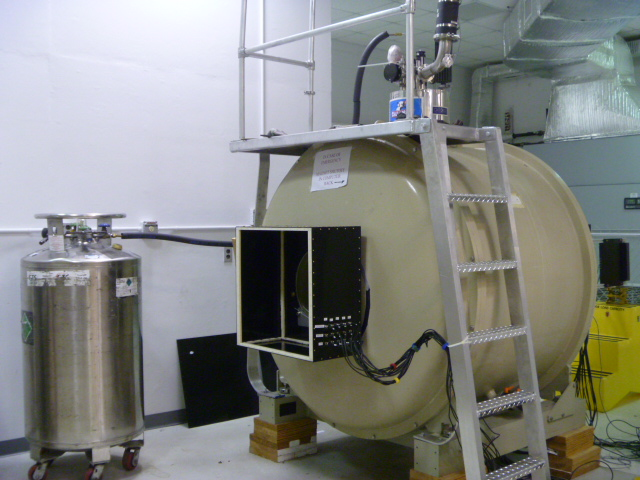
\includegraphics[width=\textwidth]{Figures/CMS_Diagrams/UVaRig__Magnet.JPG}
        \caption{The 3.8 T superconducting solenoid magnet used at UVa
        to study VPT performance}\label{fig:uva_vpt_rig_magnet}
      \end{subfigure}
      ~ %add desired spacing between images, e. g. ~, \quad, \qquad, \hfill etc.
      % (or a blank line to force the subfigure onto a new line)
    \begin{subfigure}[h]{0.450\textwidth}
        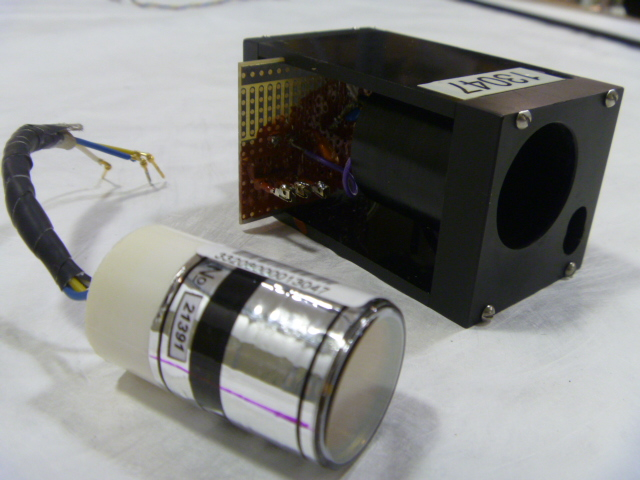
\includegraphics[width=\textwidth]{Figures/CMS_Diagrams/UVaRig__VPT_and_Housing.JPG}
        \caption{A VPT before being installed in the rig and the
          housing that provides mechanical support and high voltage connections}\label{fig:uva_vpt_rig_vpt_and_house}
      \end{subfigure}
       ~ %add desired spacing between images, e. g. ~, \quad, \qquad, \hfill etc.
      % (or a blank line to force the subfigure onto a new line)
    \begin{subfigure}[h]{0.450\textwidth}
        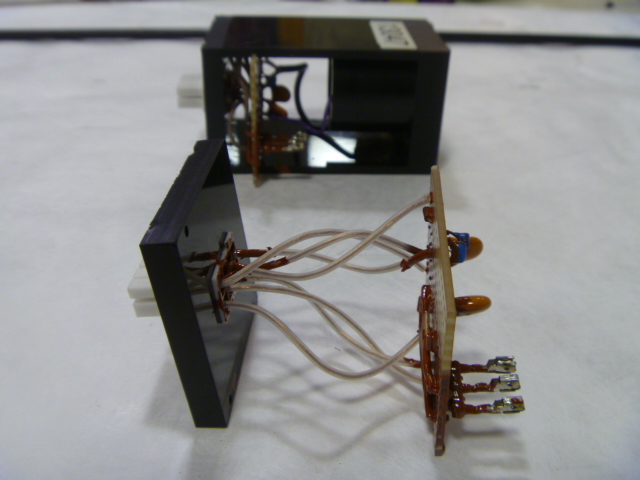
\includegraphics[width=\textwidth]{Figures/CMS_Diagrams/UVaRig__HV_filtering.JPG}
        \caption{The housing for the VPT also provides simple HV
          filtering to provide stable power to the device}\label{fig:uva_vpt_rig_hv_filter}
      \end{subfigure}
       ~ %add desired spacing between images, e. g. ~, \quad, \qquad, \hfill etc.
      % (or a blank line to force the subfigure onto a new line)
    \begin{subfigure}[h]{0.450\textwidth}
        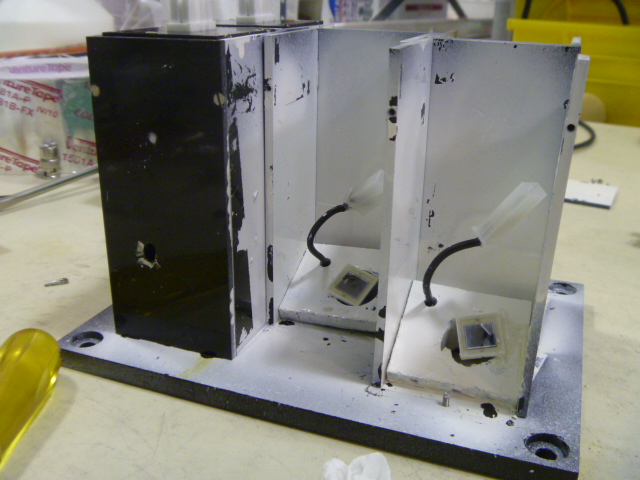
\includegraphics[width=\textwidth]{Figures/CMS_Diagrams/UVaRig__PIN_and_Housing.JPG}
        \caption{The structure which holds 5 vpts in their housing.
          A PIN diode is used to measure the LED light and make
          corrections for fluctuations in brightness}\label{fig:uva_vpt_rig_pin_and_house}
      \end{subfigure}
      ~ %add desired spacing between images, e. g. ~, \quad, \qquad, \hfill etc.
      % (or a blank line to force the subfigure onto a new line)
    \begin{subfigure}[h]{0.650\textwidth}
        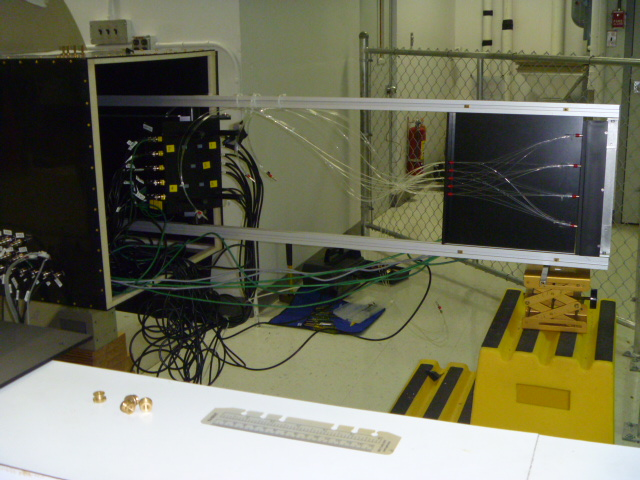
\includegraphics[width=\textwidth]{Figures/CMS_Diagrams/UVaRig__Amplifier_and_Fibers.JPG}
        \caption{The VPT rig in maintainance position outside of the
          bore of magnet (during operation the rail is instered into
          the bore such that the vpt housing is at the center).  Fiber
        optics feed from the left into the VPT and amplifier housing. }\label{fig:uva_vpt_rig_pin_and_house}
      \end{subfigure}
      \caption{Features of the UVa VPT test stand}\label{fig:uva_vpt_rig}
\end{figure}


\par The current from the VPTs anode and cathode are ultimately routed
to the PXI Crate’s switches, and then on to the crate’s DMM or
oscilloscope via a preliminary amplification stage.  The VPTs anode is
connected directly to a Stephenson amplifier, which connects to a
high-frequency switch. The PIN diode signal passes unmodified to that
same high-frequency switch. The cathode signal cables connect to a
distribution box near the PXI Crate. The distribution box then routes
their signals to the terminal block on a low-frequency switch. All of
these signals leave the rig over BNC cables before terminating at or
adjacent to the PXI Crate.  Figure \ref{fig:uva_vpt_rig} highlights
different components of the test stand at UVa.   




\subsection{Results of UVa Tests}
\label{vpt_results_description}

\par The University of Virginia rig ran three sets of 5 VPTs for
approximately 30 wks each in a 3.8 T magnetic field under high light
conditions from blue and orange frequencies to simulate a large light
yield found in large eta regions of the end-cap.  The large
photocurrents allowed the collection of an integrated charge of
$\sim$48 mC for the largest gain VPT, and 
$\sim$16 mC for the other three.   All VPTs were characterized by an
initial steep decline followed by a plateau region, which was fit with
a double exponential function of the form   

\begin{equation}
f(x) = A + B\exp {(Cx)} + D\exp {(Ex)}
\end{equation}

\begin{figure}[h]
   \centering
  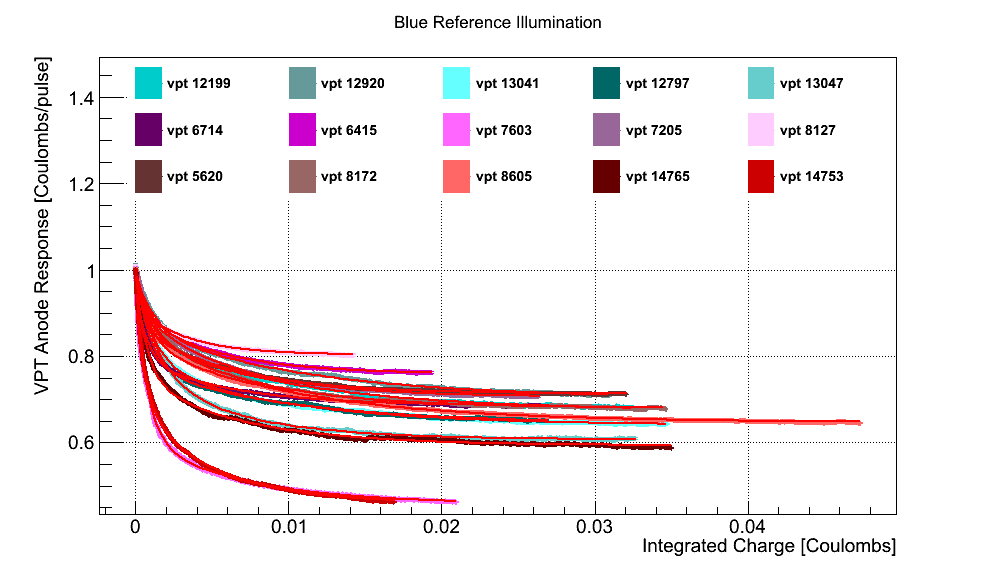
\includegraphics[width=0.9\textwidth]{Figures/CMS_Diagrams/UVaRig__all_good_runs_Overlay___blue_reference_anode__vs__integrated_charge__rolling_average_of_10pts__normalized_to_start_of_run__fitted_with_Double_Exponential.png}
  \caption{3 runs of 5 VPTs, exposed to blue LED light, and fit to a
    sum of two exponentials.} \label{fig:uva_rig_blue_fit}
\end{figure}

\begin{table}[ht] 
\begin{adjustwidth}{-1.7in}{-1.7in} 
  \centering 
  \noindent 
  \small 
    \caption{Fit Results for VPT Conditioning Studies at U.Va. and Brunel, Blue Reference LED} 
    \label{tab:UVaRig_blue} 
    \begin{tabular}{|c|c|c|c|c|c|c|c|} \hline 
RIE Number & $\%$ Drop & $\chi^2/NDF$ & Pedestal & Fast exp Amplitude & Fast exp $\tau$ & Slow exp Amplitude & Slow exp $\tau$  \\ \hline 
 
12199  & 30.1 & 1.20e+00 & 1.51e-09 & 3.42e-10 & -8.84e-04 & 3.85e-10 & -1.00e-02\\ \hline 
12920  & 27.0 & 7.27e-01 & 1.72e-09 & 3.16e-10 & -1.16e-03 & 4.03e-10 & -1.05e-02\\ \hline 
13041  & 33.5 & 8.46e-01 & 1.09e-09 & 3.43e-10 & -1.20e-03 & 2.46e-10 & -9.31e-03\\ \hline 
12797  & 33.6 & 1.07e+00 & 6.39e-10 & 2.18e-10 & -9.72e-04 & 1.31e-10 & -9.87e-03\\ \hline 
13047  & 38.1 & 1.06e+00 & 5.48e-10 & 1.98e-10 & -1.40e-03 & 1.49e-10 & -6.19e-03\\ \hline 
6714  & 29.3 & 8.37e-01 & 1.55e-09 & 4.10e-10 & -6.66e-04 & 2.48e-10 & -6.11e-03\\ \hline 
6415  & 23.6 & 1.28e-01 & 1.19e-09 & 1.54e-10 & -6.55e-04 & 2.20e-10 & -5.16e-03\\ \hline 
7603  & 50.3 & 3.25e+00 & 1.44e-09 & 1.02e-09 & -8.22e-04 & 4.87e-10 & -6.72e-03\\ \hline 
7205  & 29.4 & 4.53e-01 & 1.41e-09 & 2.14e-10 & -5.68e-04 & 3.94e-10 & -5.96e-03\\ \hline 
8127  & 19.6 & 1.97e-01 & 1.71e-09 & 1.82e-10 & -3.12e-04 & 2.35e-10 & -3.30e-03\\ \hline 
5620  & 27.4 & 4.57e+00 & 1.68e-09 & 2.85e-10 & -5.20e-04 & 3.68e-10 & -6.19e-03\\ \hline 
8172  & 30.3 & 8.75e+00 & 8.32e-10 & 1.52e-10 & -1.06e-03 & 2.27e-10 & -6.87e-03\\ \hline 
8605  & 32.1 & 6.94e+00 & 1.36e-09 & 3.33e-10 & -8.97e-04 & 3.94e-10 & -1.03e-02\\ \hline 
14765  & 38.9 & 2.78e+01 & 3.47e-10 & 1.37e-10 & -7.46e-04 & 9.24e-11 & -6.77e-03\\ \hline 
14753  & 52.9 & 2.53e+01 & 1.19e-09 & 7.45e-10 & -5.86e-04 & 6.10e-10 & -4.77e-03\\ \hline 
Average  & 31.0 & 4.62e+00 & 1.17e-09 & 2.94e-10 & -1.09e-03 & 1.66e-10 & -3.07e-01 \\ \hline 
    \end{tabular} 
  \end{adjustwidth} 
\end{table} 


\noindent where A is a pedestal parameter, B is the ampliture of the
fastest dropping exponential, C is the time constant of the fast
dropping exponential, D is the amplitude of the slow dropping
exponential, and E is the time constant of the fast exponential.  The
summary of the fit parameters for blue LED light is shown in table
\ref{tab:UVaRig_blue} and the summary of fit parameters for the orange
LED light is shown in table \ref{tab:UVaRig_orange}.  Plots of the VPT
anode response versus integrated charge, and the associated fit for
each of the devices is shown in figure \ref{fig:uva_rig_blue_fit} for
blue LED exposure and in figure \ref{fig:uva_rig_orange_fit} for
orange LED exposure.  Based on these findings, it can be concluded
that the VPT "burn-in'' eventually reaches a platea at about
$\sim70\%$ for blue LED exposure and $\sim50\%$ for orange LED
exposure.  

\begin{figure}[h]
   \centering
  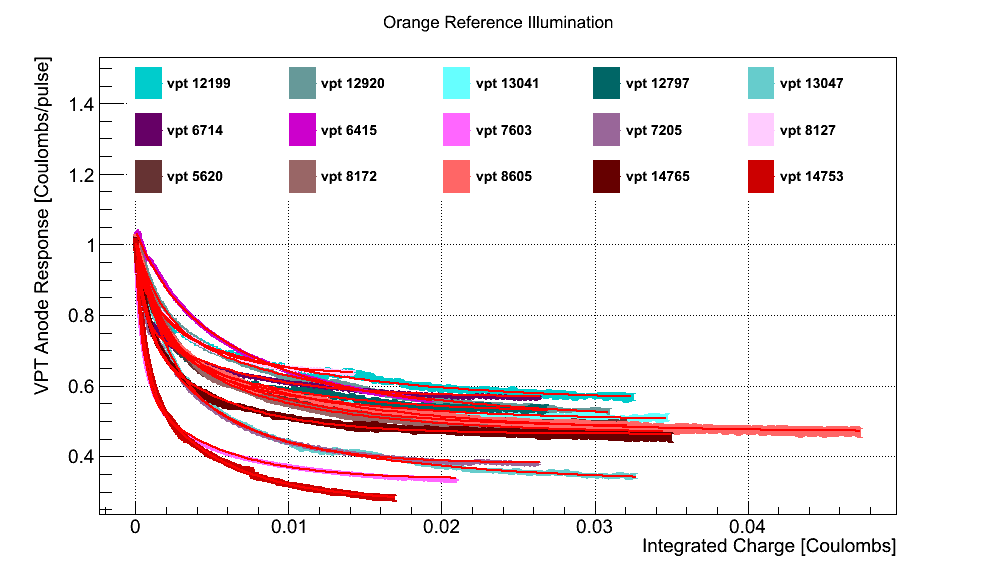
\includegraphics[width=0.9\textwidth]{Figures/CMS_Diagrams/UVaRig__all_good_runs_Overlay___orange_reference_anode__vs__integrated_charge__rolling_average_of_10pts__normalized_to_start_of_run__fitted_with_Double_Exponential.png}
  \caption{3 runs of 5 VPTs, exposed to orange LED light, and fit to a
    sum of two exponentials. } \label{fig:uva_rig_orange_fit}
\end{figure}

\begin{table}[ht] 
\begin{adjustwidth}{-1.7in}{-1.7in} 
  \centering 
  \noindent 
  \small 
    \caption{Fit Results for VPT Conditioning Studies at U.Va., Orange LED} 
    \label{tab:UVaRig_orange} 
    \begin{tabular}{|c|c|c|c|c|c|c|c|} \hline 
RIE Number & $\%$ Drop & $\chi^2/NDF$ & Pedestal & Fast exp Amplitude &  Fast exp $\tau$  & Slow exp Amplitude &  Slow exp $\tau$   \\ \hline 
 
12199  & 41.9 & 6.23e-01 & 4.23e-10 & 1.79e-10 & -1.10e-03 & 1.76e-10 & -1.10e-02\\ \hline 
12920  & 45.3 & 1.84e-01 & 6.73e-10 & 3.24e-10 & -1.67e-03 & 3.72e-10 & -1.26e-02\\ \hline 
13041  & 48.3 & 7.42e-01 & 2.75e-10 & 1.81e-10 & -1.63e-03 & 1.04e-10 & -1.02e-02\\ \hline 
12797  & 46.4 & 5.05e-01 & 2.05e-10 & 1.14e-10 & -1.23e-03 & 7.87e-11 & -8.77e-03\\ \hline 
13047  & 63.0 & 1.09e+00 & 1.34e-10 & 1.73e-10 & -2.18e-03 & 1.07e-10 & -1.16e-02\\ \hline 
6714  & 43.4 & 1.43e+01 & 7.73e-10 & 3.29e-10 & -4.49e-04 & 2.84e-10 & -6.11e-03\\ \hline 
6415  & 46.5 & 2.34e+01 & 4.41e-10 & 8.75e-11 & -1.80e-03 & 3.47e-10 & -7.95e-03\\ \hline 
7603  & 64.8 & 3.20e+01 & 3.01e-10 & 3.42e-10 & -5.42e-04 & 2.24e-10 & -5.04e-03\\ \hline 
7205  & 63.2 & 6.52e+01 & 1.94e-10 & 1.29e-10 & -4.49e-04 & 2.16e-10 & -5.13e-03\\ \hline 
8127  & 39.4 & 2.24e+01 & 7.09e-10 & 1.54e-10 & -2.08e-04 & 3.10e-10 & -3.75e-03\\ \hline 
5620  & 50.3 & 2.30e-01 & 4.07e-10 & 2.13e-10 & -1.16e-03 & 2.37e-10 & -7.79e-03\\ \hline 
8172  & 51.7 & 1.56e-01 & 4.01e-10 & 2.73e-10 & -1.91e-03 & 2.08e-10 & -9.48e-03\\ \hline 
8605  & 49.6 & 1.83e-01 & 2.39e-10 & 1.46e-10 & -1.45e-03 & 1.33e-10 & -1.12e-02\\ \hline 
14765  & 53.3 & 3.08e-01 & 2.07e-10 & 1.27e-10 & -8.55e-04 & 1.17e-10 & -5.66e-03\\ \hline 
14753  & 72.2 & 2.22e-01 & 1.94e-10 & 2.76e-10 & -6.01e-04 & 2.47e-10 & -5.06e-03\\ \hline 
Average  & 52.0 & 1.08e+01 & 3.72e-10 & 2.03e-10 & -1.15e-03 & 2.11e-10 & -8.10e-03 \\ \hline 
    \end{tabular} 
  \end{adjustwidth} 
\end{table} 
 

\section{The Hadronic Calorimeter}
\label{hcal_description}

\begin{figure}[h]
   \centering
  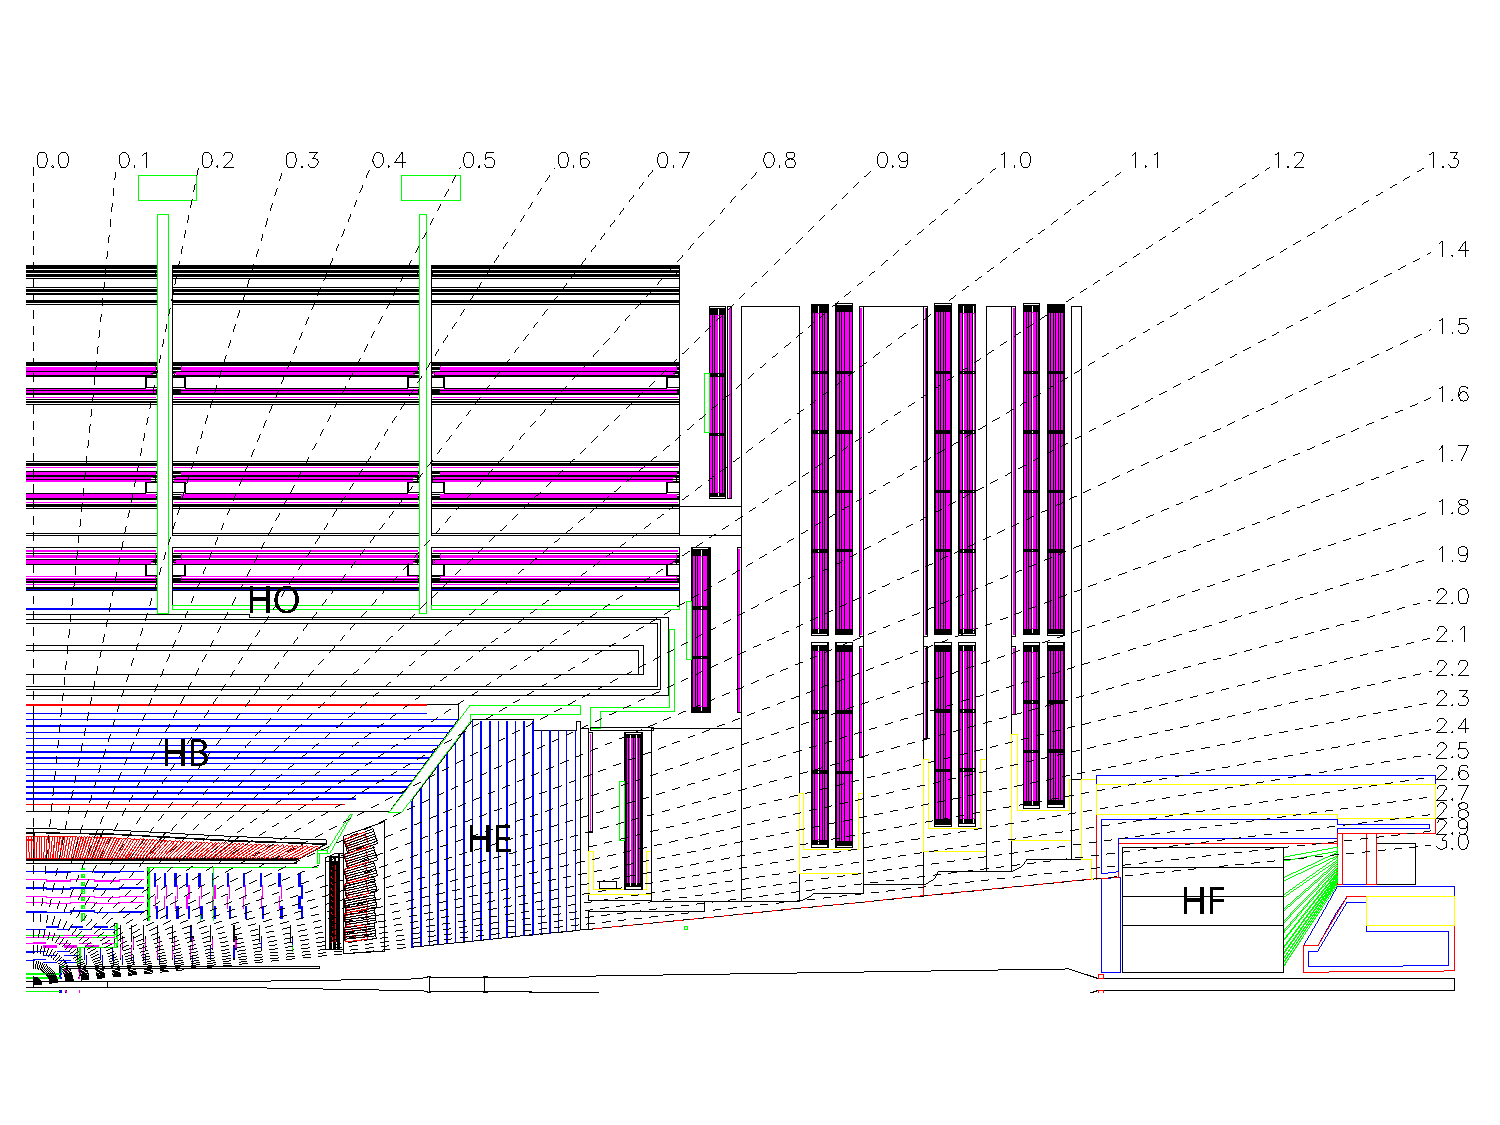
\includegraphics[width=0.9\textwidth]{Figures/CMS_Diagrams/HCAL__Layout.pdf}
  \caption{Longitudinal cross-section of the HCAL with the four
    sub-systems labeled} \label{fig:hcal_layout}
\end{figure}

\par The \acrfull{hcal} is is divided into four sub-systems: the
barrel (HB), the endcap (HE), the outer calorimeter (HO), and the
forward calorimeter (HF).   It is especially important for measuring
hadronic jets and neutrinos by measuring an imbalance in energy
transverse to the beamline.  It provides coverage from $|\eta|<3$ from
the HB, HE, and HO, and the HF extends the coverage out to
$|\eta|<5.2$.  A diagram of the longitudinal cross
section is shown in figure \ref{fig:hcal_layout}.

\begin{figure}[h]
   \centering
  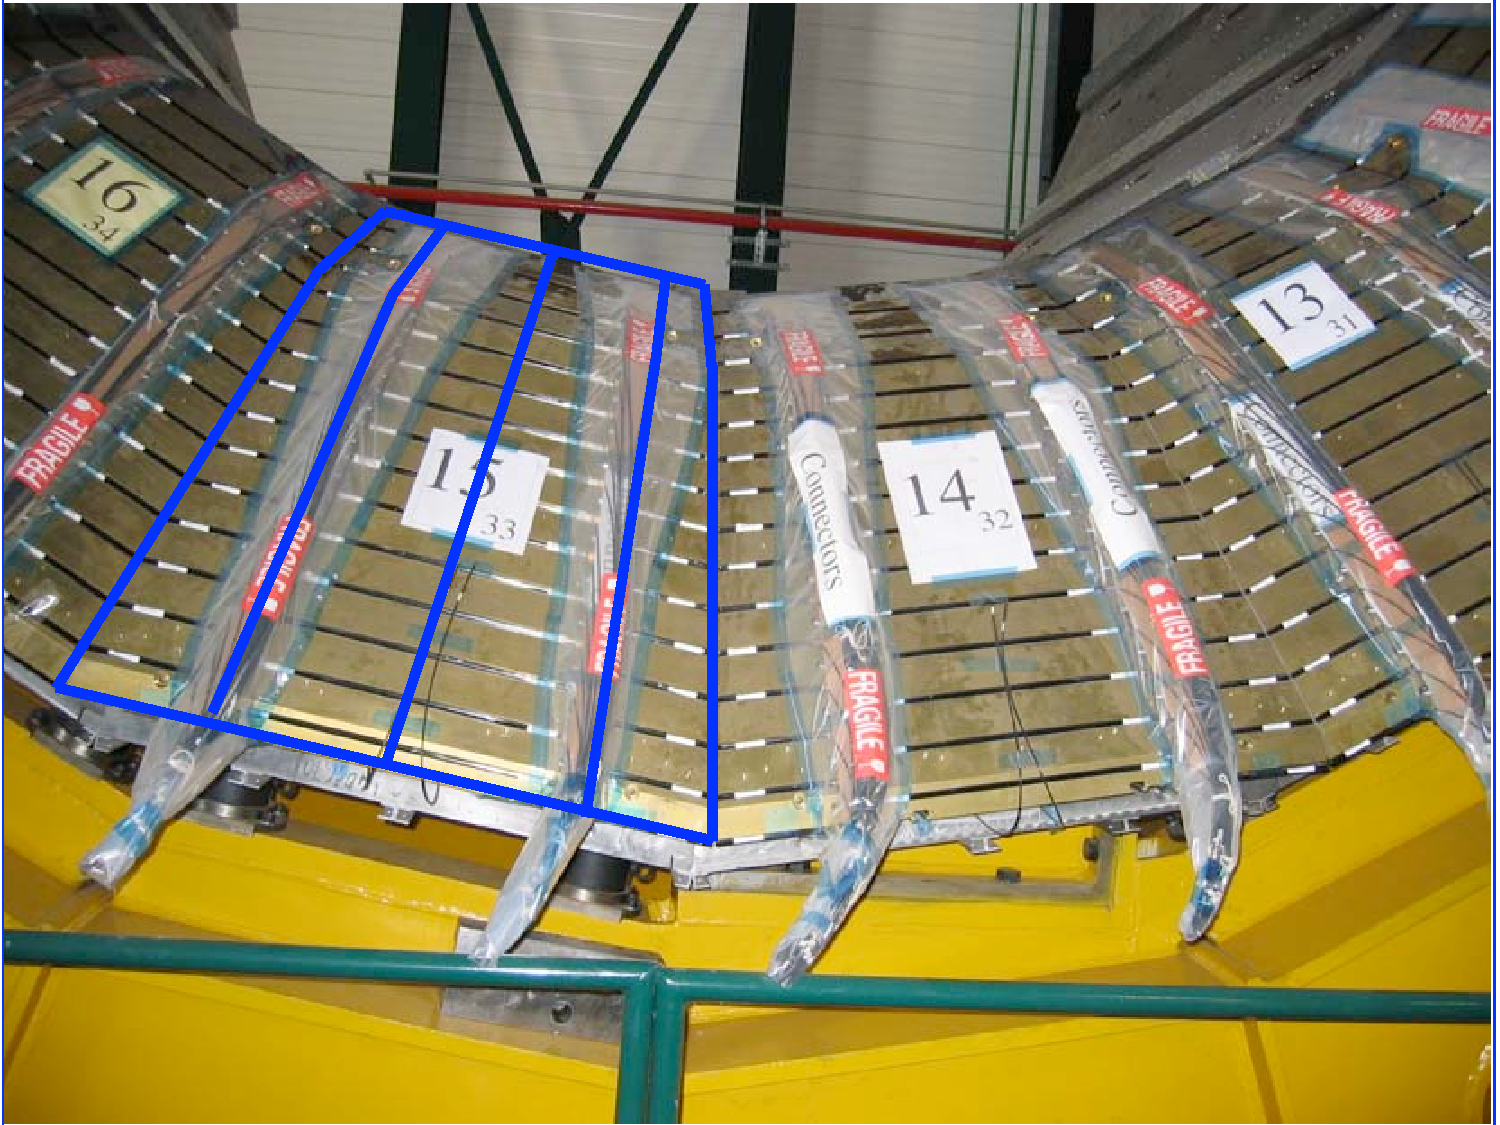
\includegraphics[width=0.8\textwidth]{Figures/CMS_Diagrams/HCAL__Wedge_WithAzDiv.pdf}
  \caption{Closeup of the HCAL barrel section.  The center section of
    each of the 18 wedges are labeled, optical cables lay accross the
    joint of the center and staggered edge sections of each wedge.
    The blue lines show the apporximate azimuthal division of the
    wedge.} \label{fig:hcal_hb_wedge}
\end{figure}

\par The barrel section of the HCAL, the HB, is divided into two
sections longitudinaly, each with 18 identical azimuthal wedges
wrapped around the beamline.  Each wedge has four azimuthal sections,
with the center two sections aligned and each edge piece angled and
staggered in a configuration that creates no projective dead material
for the full radial extent of the HCAL.  Figure
\ref{fig:hcal_hb_wedge} shows a closeup photograph of four wedges,
where optical fibers are layed out accross the seam that joins the
staggered edge layers to the two aligned center layers, and blue lines
highlight the four azimuthal divisions for a single wedge.  

\begin{figure}[h]
   \centering
  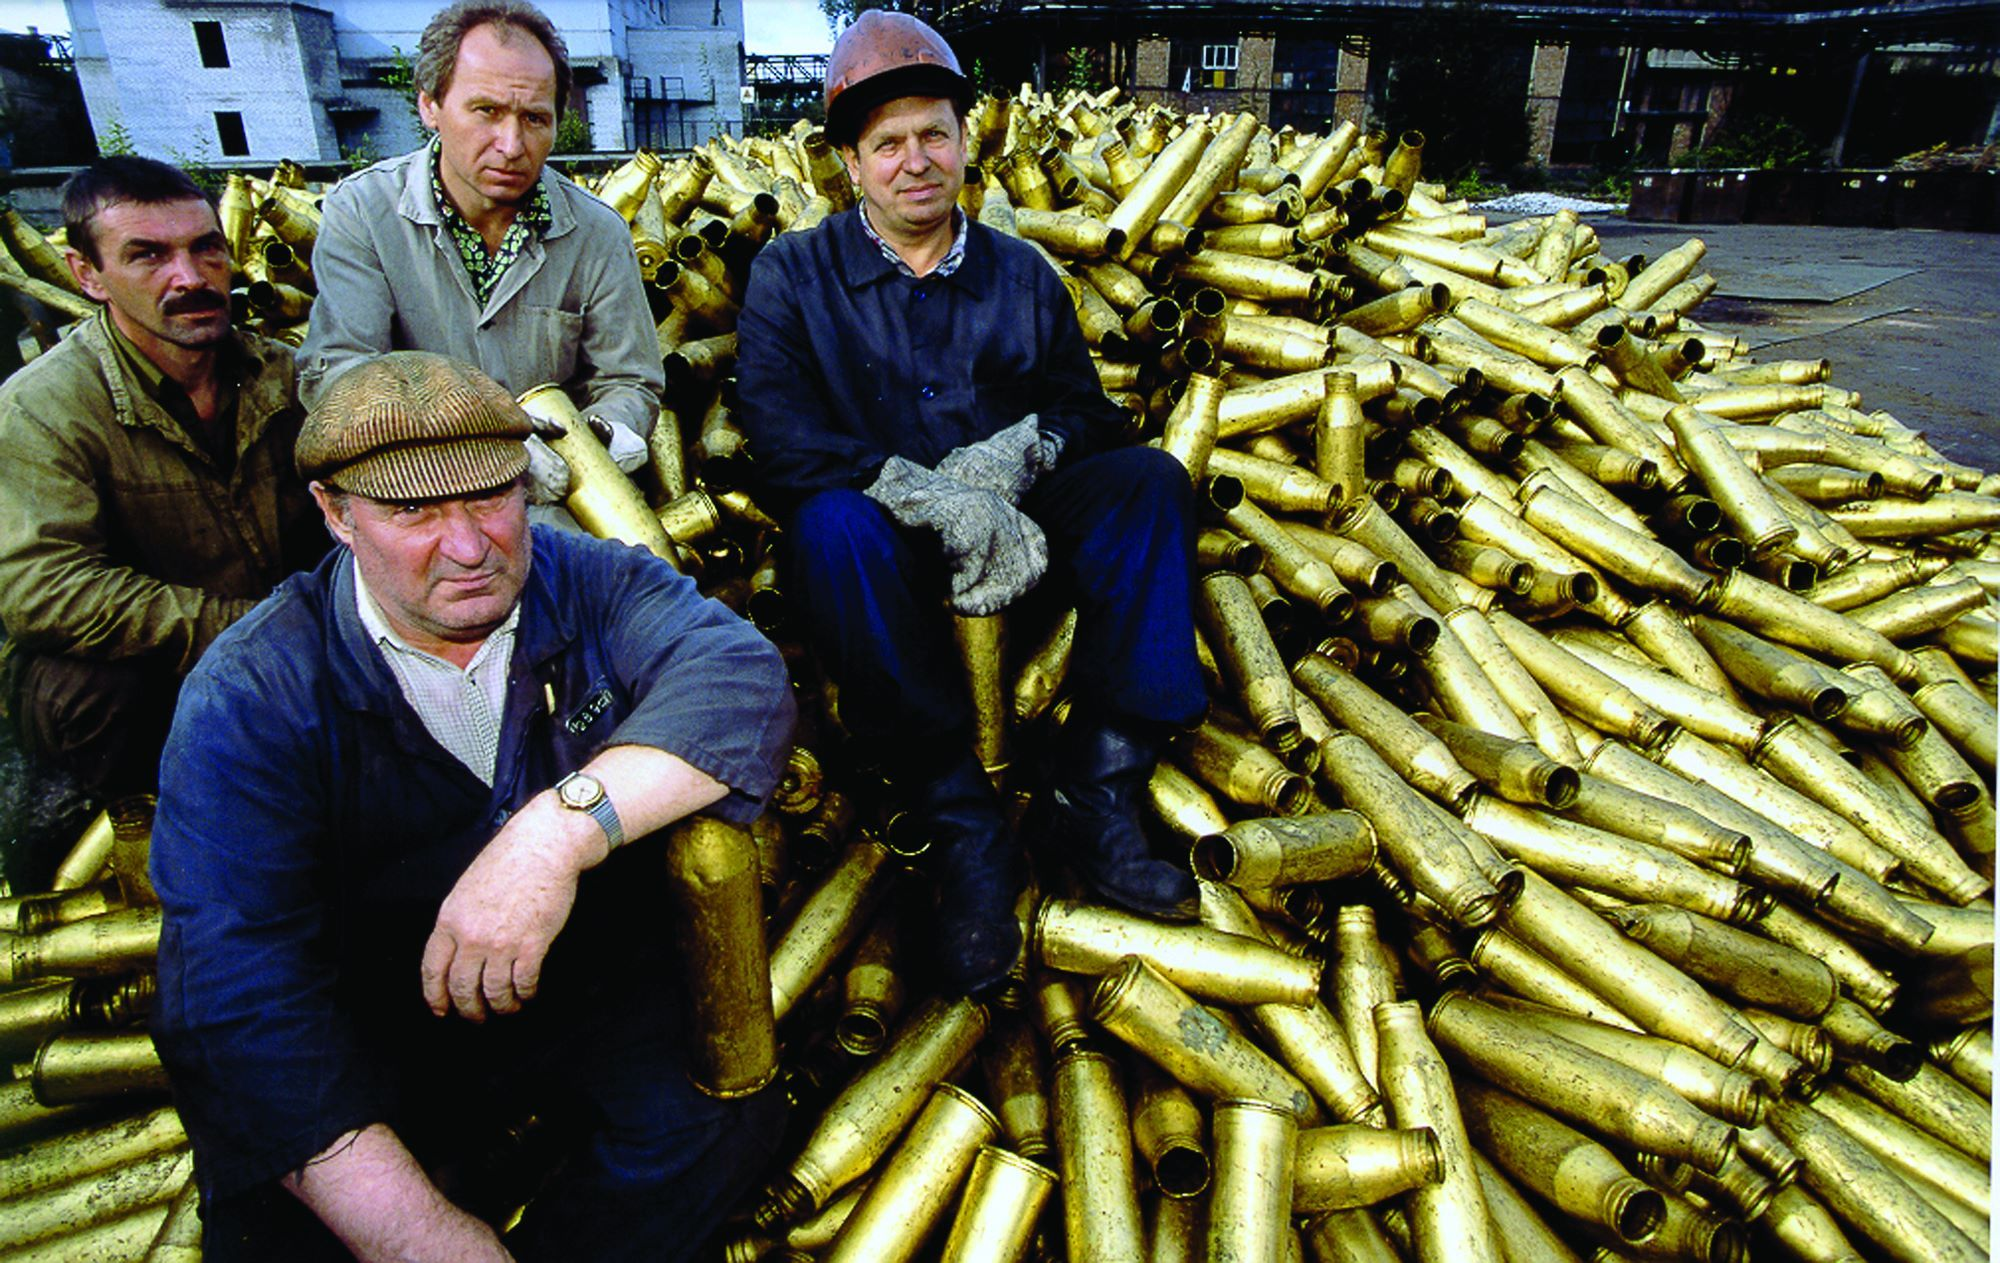
\includegraphics[width=0.7\textwidth]{Figures/CMS_Diagrams/HCAL__NavyShells.jpg}
  \caption{Over 1 million Russian shells of military artillery were
    re-processed in the construction of the HCAL} \label{fig:hcal_navy_shells}
\end{figure}

\par The HB is a sampling calorimeter, with each azimuthal section
composed of 14 alternating layers of brass absorber plates, and layers
plastic scintilator tiles, with steel plates on the top and bottom
layers for structural support.  Each quarter-barrel section of
scintillator has 16 $\eta$ divisions, giving a segmentation of
$(\Delta\eta, \Delta\phi) = (0.087, 0.087)$.  The brass absorber
plates are C26000/Cartridge Brass.  The material was chosen since the
absorber material could not be distorted or bend under the stress of
its own weight for at least 15 years of experimental running.  Much of
the material was purchased, but over a million Russian WW2 brass shell
casings, designed to withstand the stresses of travel aboard 1940s
Navy vessals, were melted down and processed into absorber tiles.
Figure \ref{fig:hcal_navy_shells} shows members of the Russian Navy
posing with some of the shells. 

\begin{figure}[h]
   \centering
  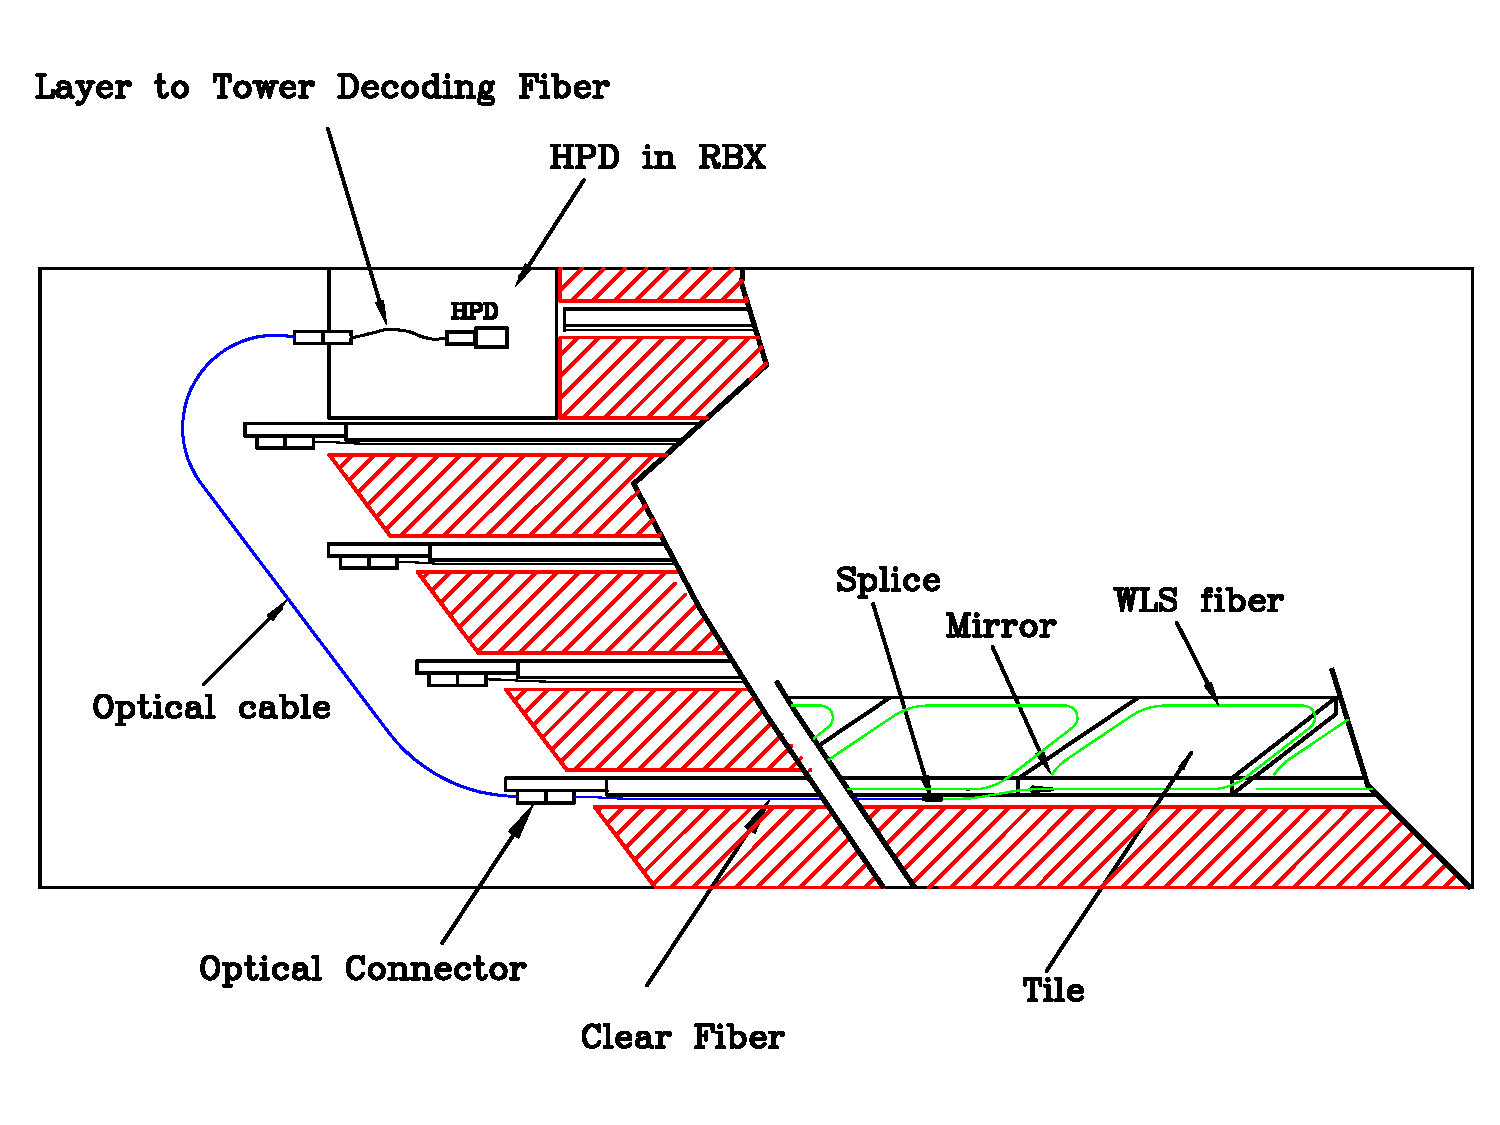
\includegraphics[width=0.7\textwidth]{Figures/CMS_Diagrams/HCAL__OpticalReadout.pdf}
  \caption{Optical readout chain of the HCAL scintiallator tiles} \label{fig:hcal_navy_shells}
\end{figure}

\par When a hadron passes through a wedge, the brass and steel plates
absorb energy and initiates the decay of the hadron into a number of
lighter particles.  These particles pass through the scintillator
layer, which absorb energy from the interactions or collisions with
the passing particles.  The electrons of the scintillator become
excited and relax by emitting a number of photons in the blue-violet
range of the visible spectrum proportional to the amount of energy
absorbed by the scintillator.   These photons are abosrbed by
wavelength shifting fibers (WSFs), which re-emit the light in the
green part of the visible spectrum.  The WSFs are spliced into 
four clear fiber optical cables.  These fibers transport the light
from each of the layers to an optical decoding unit (ODU), which
arranges the fibers into readout towers.  A hydrid photodiode (HPD)
converts this light into electric signals and is digitized by an ADC
contained on the front-end elctronics.  The HPD is a photo-cathode,
which converts light to electrons via the photoelectric effect, that
sits above a silicon diode that amplifies the signal of the cathode.
The HPD provides a gain of 2000 to the light signals received from the
scintialator trays.  The on-detector electronics communicate to the
HCAL trigger/readout (HTR) boards, which communicate with the trigger
system to decide whether the store the event as data or discard it.  

\par  The brass absorbing material has a nuclear interaction length,
or the length necesary to reduce the number of charged particles in a
hadron shower by 1/e, of 16.42 cm, and a radiation length of 1.49 cm.
This means that te HB will be able to contain a large part of most
hadron showers produced at LHC energies, but a portion will still pass
through the entire radial distance.  The outer barrel layer, HO is
designed to measure the remants of the hadron shower.  It sits outside
of the solenoid magnet, using it as an absorber layer
1.4/$\sin{\theta}$ interaction lengths.  It consists of 5 sections
along the z-axis, which form rings aorund the beamline.  Each ring is
a layer of scintilator tiles at radial distance of 4.07m, except for
the center ring.  Since it corresponds the the $\eta=0$ ring, there is
a minimum amount of absorber material in front of it.  The central
ring is thus two layers of scintiallator at radial distances 3.82 and
4.07 m, which sit on either side of a 19.5cm thick piece of iron
absorber.  

\begin{figure}[h]
   \centering
  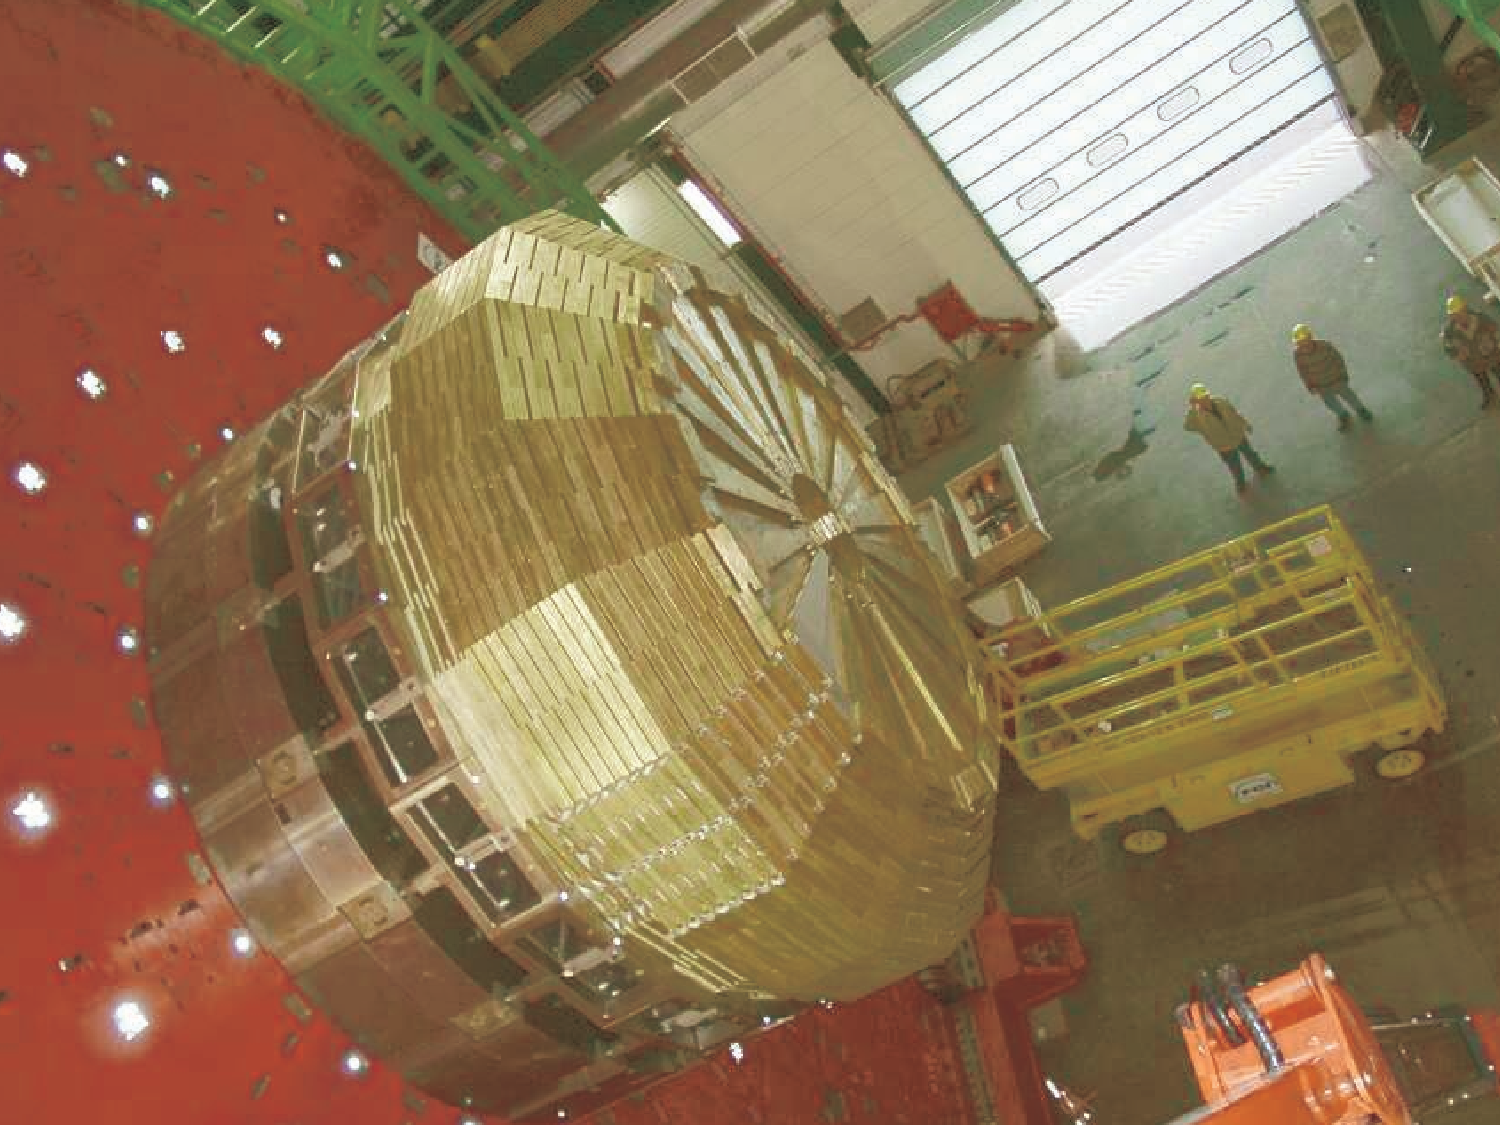
\includegraphics[width=0.7\textwidth]{Figures/CMS_Diagrams/HCAL__Endcap.pdf}
  \caption{HCAL endcap, 18 azimuthal divisions of alternating layers
    of brass and plastic scintillator.} \label{fig:hcal_endcap}
\end{figure}

\par The endcap system, the HE, provide a substantial portion of the total
$\eta$ coverage, from $1.3<|\eta|<3.0$, and contains $\sim$1/3 of the
final state particles in a collision.  Like the HB, it is a sampling
calorimeter with alternating layers of brass and plastic.  The demand
for radiation hardness, and the need for a non-magnetic material, lead
to the same choice of C26000 cartidge brass found in the HB.  It is
also divided into 18 azimuthal wedges, and 16 $\eta$ divisions, giving
it the same $(\Delta\eta, \Delta\phi) = (0.087, 0.087)$ segmentation.
Figure \ref{fig:hcal_endcap} shows an image of a partially assembeled
endcap before being installed.

\begin{figure}[h]
   \centering
  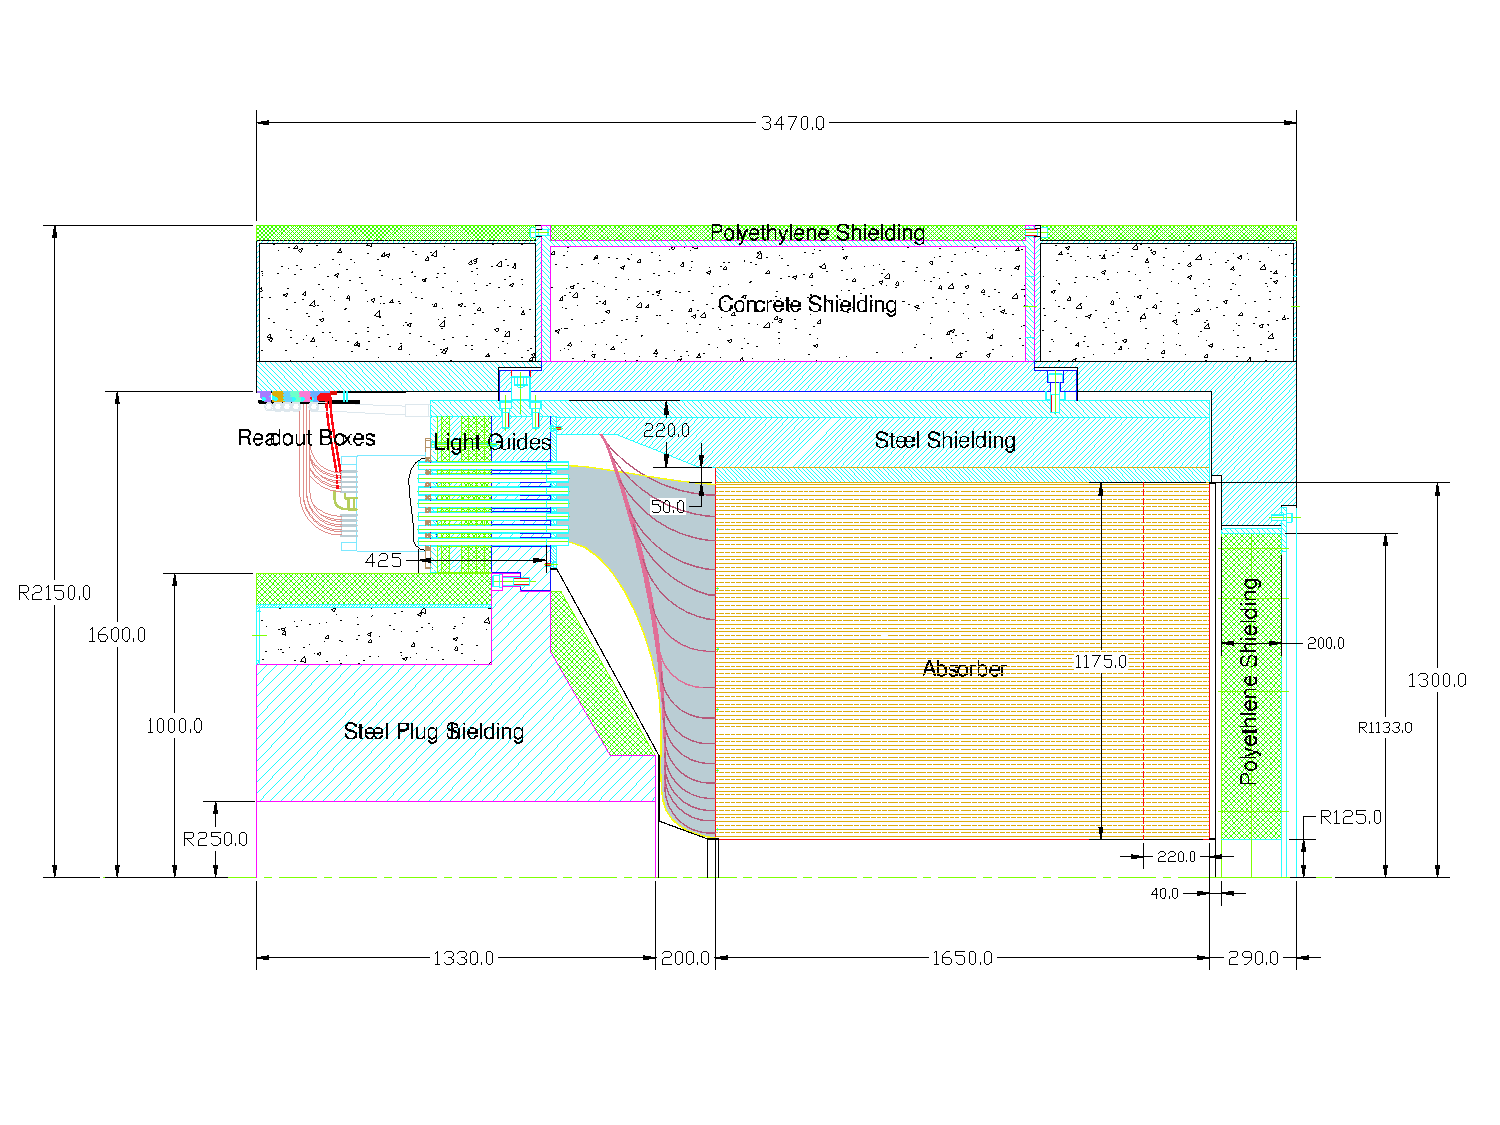
\includegraphics[width=0.8\textwidth]{Figures/CMS_Diagrams/HCAL__HF_layout.pdf}
  \caption{Longitudinal cross-section of the HCAL forward calorimetry,
  the HF} \label{fig:hcal_hf_layout}
\end{figure}

\par The forward calorimetry, HF, extends the HCAL coverage from
$3.0<|\eta|<5.0$, and necessarily must sit in the region of the
detector with the largest particle fluxes and thus radiation
exposure.  The HF is a cylindrial steel structure with an inner bore
12.5 cm from the beam line, and a outer radius of 130.0 cm.  It sits
11.2 m  away from the nominal interaction point in the $\hat{z}$
direction.  Like the HE, it has 18 azimuthal divisions on either side
of the interaction point.  Relativistic particles that move through
the steel generate Cherenekov light, which is collected by radiation
hard quartz fibers, which transport the light to HPDs which are
readout in the manner as described above.  Since the detection
mechanism is Cherenekov light, this sub-system is primarily sensity to
the electromagnetic component of the hadronic shower.  Figure
\ref{fig:hcal_hf_layout} shows a cross-sectional view of the HF
detector.   

%\section{Forward Caliorimetry}
%\label{fcal_description}
%
%\par High eta, great for VBF
%
%\section{Magnet and Return Yoke}
%\label{magnet_description}
%
%\par Describe solenoid and measuring field, and engineering marvel or
%return yoke structure.
%

\section{Muon Chambers}
\label{muon_chamber_description}

\par In $pp$ collisions, muons are only created through electroweak or
exotic physics processes, making the detection of this particle an
invaluable tool for reducing the large hadronic backgrounds produced
at the LHC.  The muon chambers, positioned furthest from the beamline,
sit behind the ECAL and HCAL detectors, which absorb almost all of the
hadronic activity from a collision.  They operate in a relatively low
flux environment, allowing for robust measurement of their
kinematics, making it an excellent trigger system.  One of the most
imortant discovery channels for the  Higgs bosn, involved the decay of
the Higgs into two $Z$ bosons, which decay to two pairs of muons.
Only 25 events were needed for a statistically significant observation
in that channel, since the backgrounds had been reduced to only 5
expected events and the muons had provided high resolution on the
invariant mass of the Higgs.   

\par The muon chambers are composed of three types of gaseous detector
technology: drift tubes (DTs), cathode strip chambers (CSCs), and
resistive plate chambers (RPCs).  In the muon barrel system (MB),
where the magnetic field is uniform DTs provide $\eta$ coverage, for
$|\eta|<1.4$, and are supplemented by a system of RPCs that provide an
independent trigger source and faster timing resolution.  In the muon
endcap system (ME), where the magnetic field would degrade the
performance of DTs, a system of CSCs and RPCs provide $\eta$ coverage
from $1.4<|\eta|<2.4$.  

\begin{figure}[h]
   \centering
  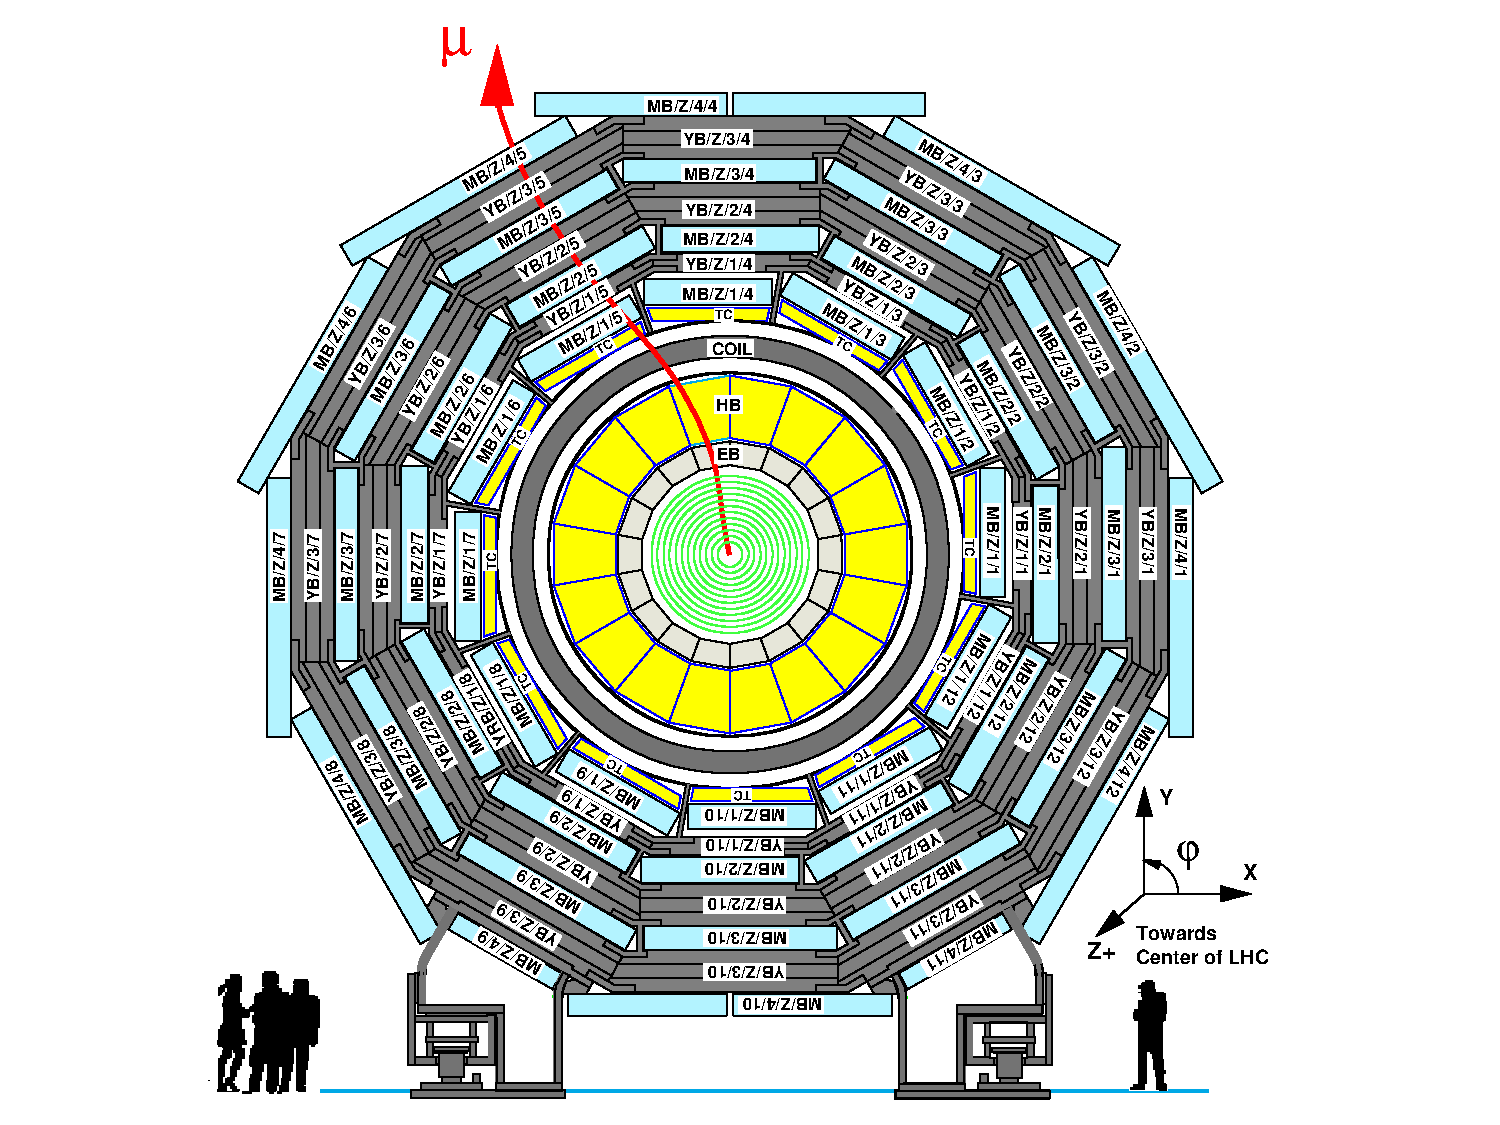
\includegraphics[width=0.85\textwidth]{Figures/CMS_Diagrams/Muon__DT_layout.pdf}
  \caption{Longitudinal cross-section of one of the 5 wheels of the
    muon system.  Drift tubes are placed in 4 concentric layers, with
    2 being placed inside the return yoke of the magnet, and 12
    azimuthal divisions.} \label{fig:muon_dt_layout}
\end{figure}

\begin{figure}[h]
   \centering
  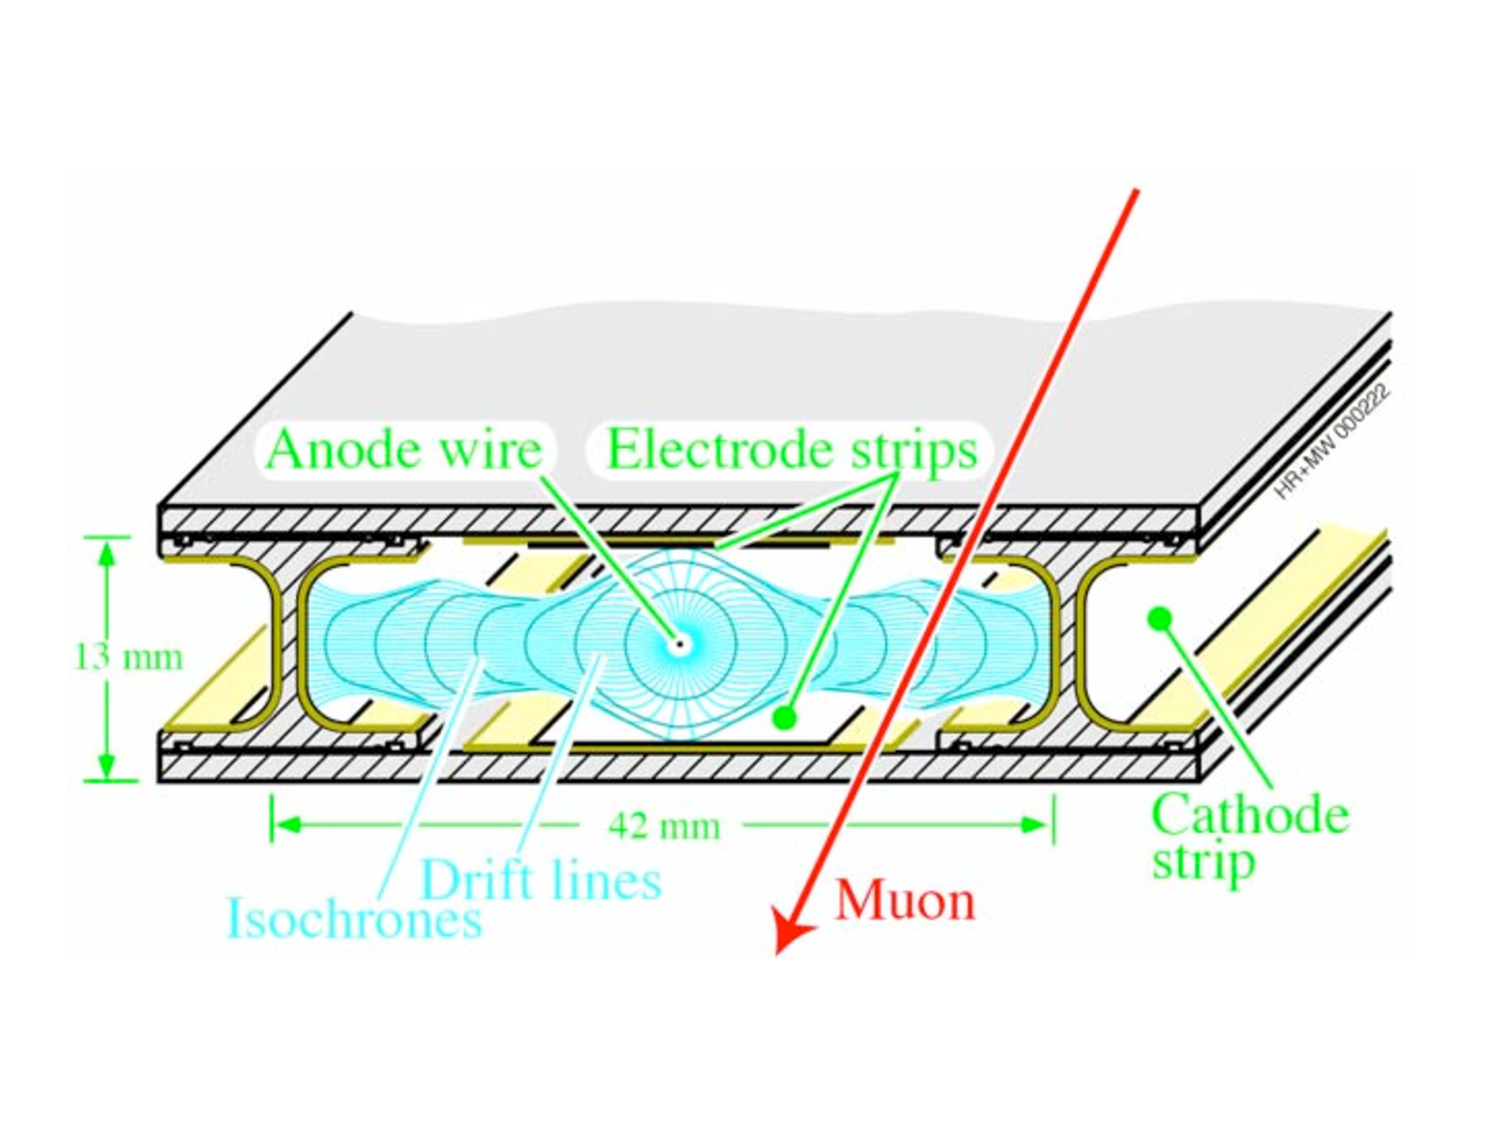
\includegraphics[width=0.85\textwidth]{Figures/CMS_Diagrams/Muon__DT_cell.pdf}
  \caption{A cross-section view of a drift cell.  The anode wire is
    held at 3600 V, creating a potential difference with the walls.
    Electric field lines are shown in blue.} \label{fig:muon_dt_cell}
\end{figure}

\par The DTs are located in the MB system, which is divided into 5
longitudanal, cylindrical sections around the beamline, known as
wheels.  In each wheel there there 4 concentric layers of drift tube
stations, one on either side of the magnet return yoke, and two
interspersed inside of it.  Each wheel is divided intwo 12 azimuthal
section, making 48 stations in the barrel, as shown in figure
\ref{fig:muon_dt_layout}.  Each station on the first three (fourth)
layers contain 3(2) superlayers, where each superlayer is made of a
stack of 4 layers of rectangular drift cells, which are staggered by
half a cell each.  Two of the superlayers are oriented such that they
are parallel to the beam, measuring the muon in the $r-\phi$ plane.
The first three layers contain a third superlayer, orientated
perpendicular to the beam, measuring a $z$ component of the muon
trajectory.  Each drift cell is a hollow 13$\times$42 mm tube, with a
relatively thick 1.5mm wall to provide isolation between adjacent
cells.  Each cell is filled with a mixture of 85$\%$ argon + 15$\%$
CO$_{2}$ gas mixture, and contains an anode wire that is held at 3600
V that runs down the axis of the cell.  The walls of the cell are held
at 1800 V or -1200 V depending on the wall.  When a muon passes
through the chamber, it's charge ionizes molecules of the CO$_{2}$
gas, causing the electrons to drift towards the anode wire, and the
CO$_{2}$ ions drift towards the wall.  As the electrons approach the
anode, they are accelerated and liberate secondary elctrons from other
CO$_{2}$ molecules, creating an avalanche of electrons near the wire,
resulting in a drop in voltage as they are collected.  The voltage
drop is read out by front end electronics as a signal that a muon has
passed through the chamber.  The Argon gas quenches the avalanche
reaction, and the maximum drift time for electrons in the gas is 380
ns.  This long time scale necessitates the use of an addtional,
fast-timing system, the RPCs.  Figure \ref{fig:muon_dt_cell} shows a
cross-section view of a drift cell, including electric field lines
produced by the potential difference between the anode wire and the
walls of the drift cell.   

\begin{figure}{h}
    \centering
    \begin{subfigure}[h]{0.40\textwidth}
        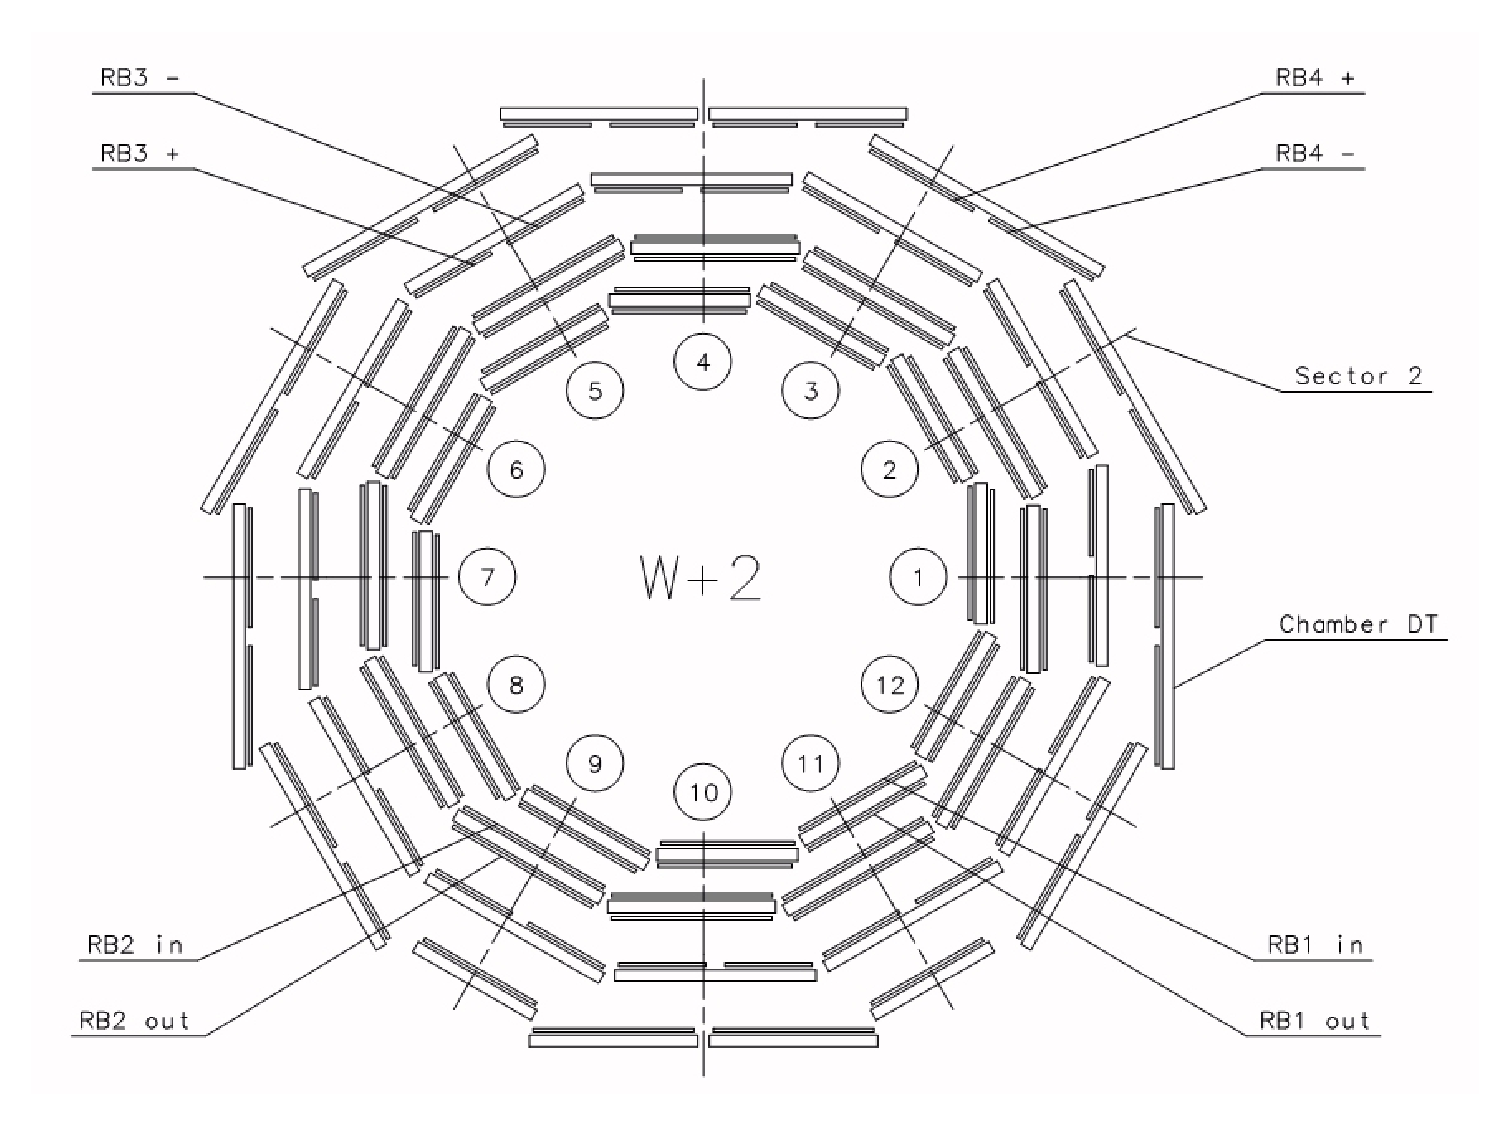
\includegraphics[width=\textwidth]{Figures/CMS_Diagrams/Muon__RPC_barrel_layout.pdf}
        \caption{A longitudinal cross-section of the muon barrel RPC
          system.  RPCs are attached to the top and bottom of the
          first two layers of drift stations, and to the bottom of the
        outer two layers}\label{fig:muon_rpc_barrel_layout}
      \end{subfigure}
      ~ %add desired spacing between images, e. g. ~, \quad, \qquad, \hfill etc.
      % (or a blank line to force the subfigure onto a new line)
    \begin{subfigure}[h]{0.40\textwidth}
        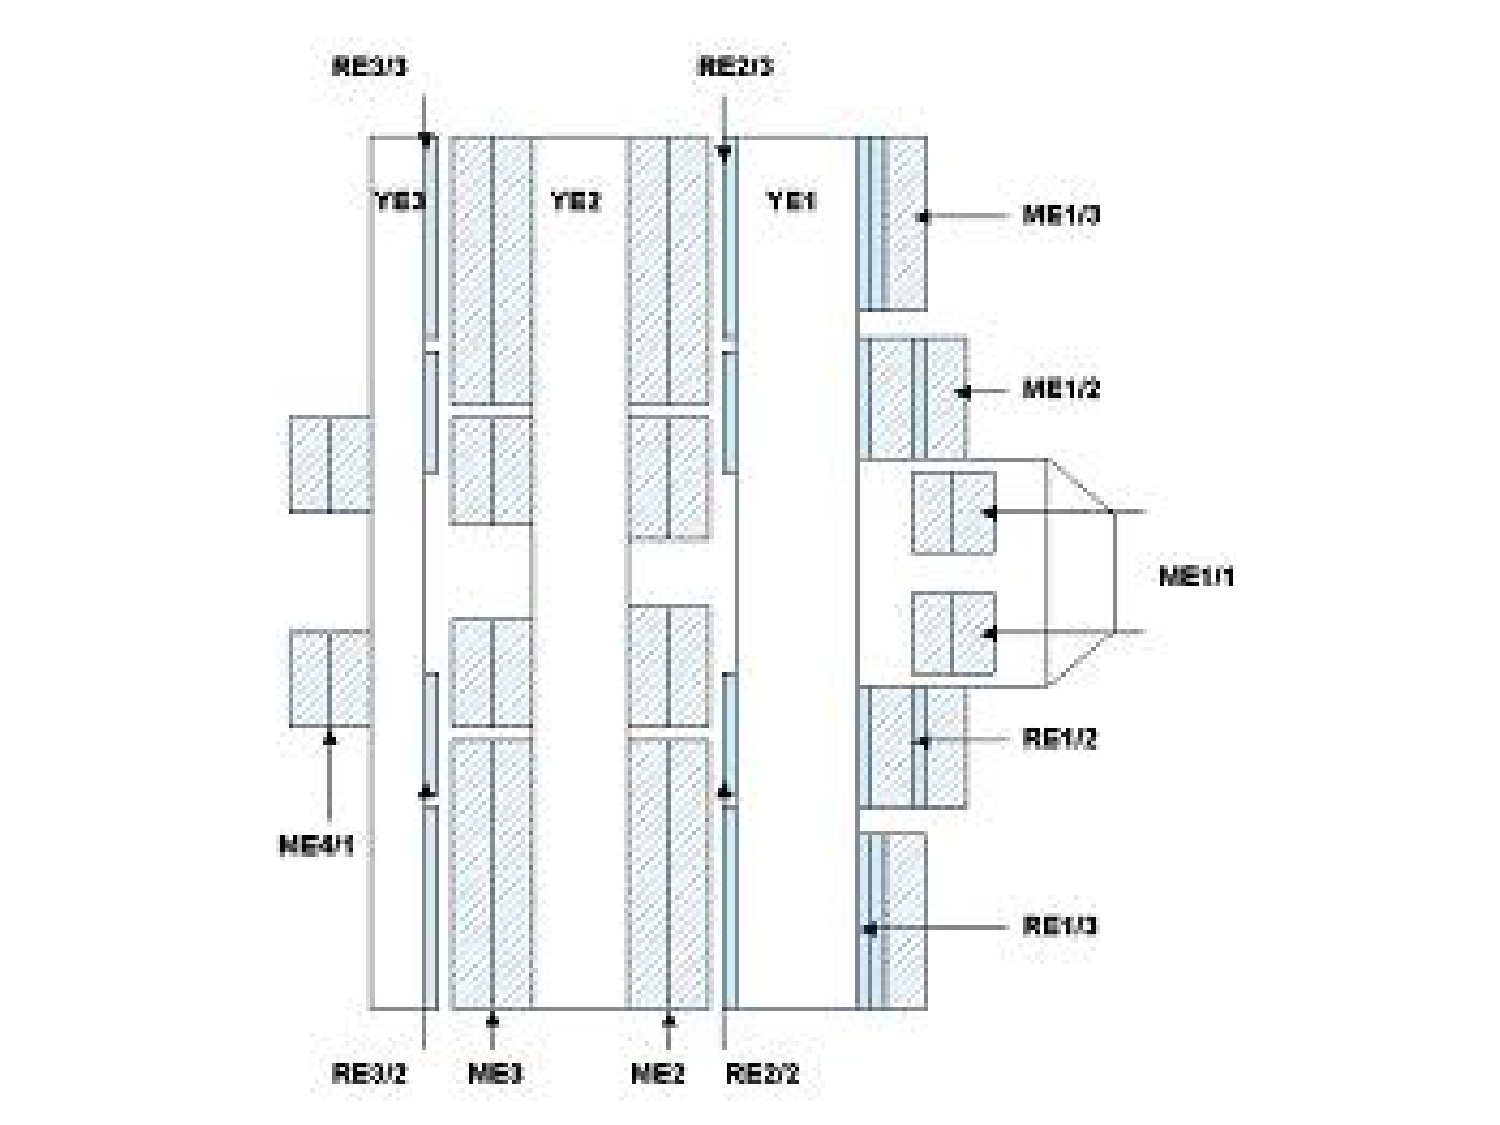
\includegraphics[width=\textwidth]{Figures/CMS_Diagrams/Muon__RPC_endcap_layout.pdf}
        \caption{Cross-section of muon endcap system.  It is composed
          of three disks, with RPCs mounted on the back of CSC system
          on the first and last disks, and on the front of the CSC in the middle disk}\label{fig:muon_rpc_endcap_layout}
      \end{subfigure}
      \caption{RPC layout for the barrel and endcaps}\label{fig:muon_rpc_layout}
\end{figure}

\begin{figure}[h]
   \centering
  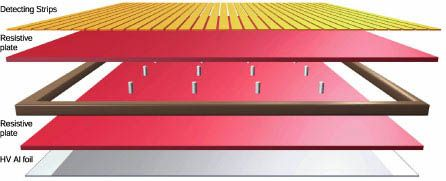
\includegraphics[width=0.6\textwidth]{Figures/CMS_Diagrams/Muon__RPC_schematic.jpg}
  \caption{Exploded diagram of an RPC} \label{fig:muon_rpc}
\end{figure}

\par The reisistive place chambers (RPCs) are the fast timing system
chosen to supplement the DTs in the barrel, and the CSCs in the
endcaps.  In the barrel, they are adhered to the top and bottom of the
first two layers of drift stations.  In the outer two layers, they are
only adhered to the bottom of each station.  Figure
\ref{fig:muon_rpc_layout}(\subref{fig:muon_rpc_barrel_layout}) shows the
layout of the barrel RPC system.  The muon endcap system is composed
of three disks on either side of the intreraction point, and is shown
in figure
\ref{fig:muon_rpc_layout}(\subref{fig:muon_rpc_endcap_layout}).  RPCs
are mounted on the back of the CSC stations of the innermost and
outermost disks, and on the front of the CSC for the middle disk. Each
RPC consists of two plates of high resistance material, one held at a
postive voltage, the anode, and the other held at a negative voltage, 
the cathode.  The volume between the plates is filled with a gas
similar to the drift tubes.  When a muon passes between the plates, it
ionizes the gas molecules, and the electrons are accelerated towards
the positive plate, creating an avalance of secondary electrons that
combine with the positive plate creating a voltage drop that is read
out as a signal.  The timing resolution acheived from the RPCs is less
than the 25 ns LHC bunch crossing, supplementing the spatial
resolution provided by the DTs in the barrel, and the CSCs in the
endcap.  

\begin{figure}[h]
   \centering
  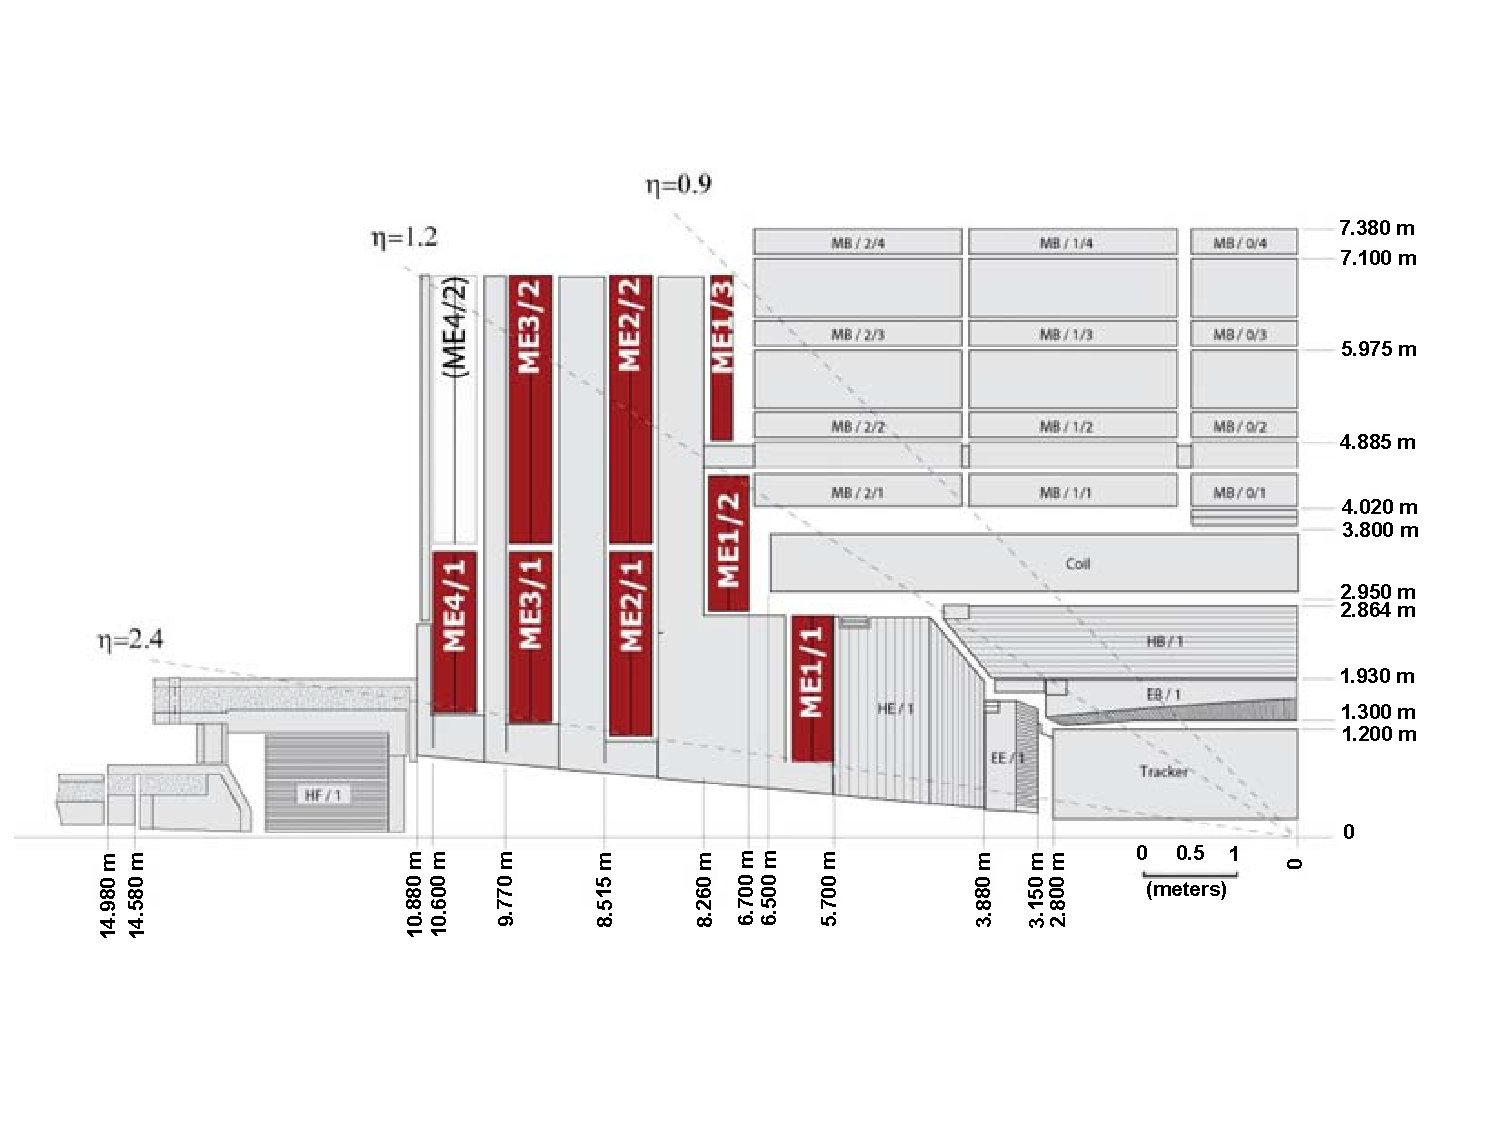
\includegraphics[width=0.6\textwidth]{Figures/CMS_Diagrams/Muon__Endcap_CSC_layout.pdf}
  \caption{Cross-section of one quarter of the muon endcap system,
    with the 4 disks of CSC systems shown in red} \label{fig:muon_csc_layout}
\end{figure}

\begin{figure}[h]
   \centering
  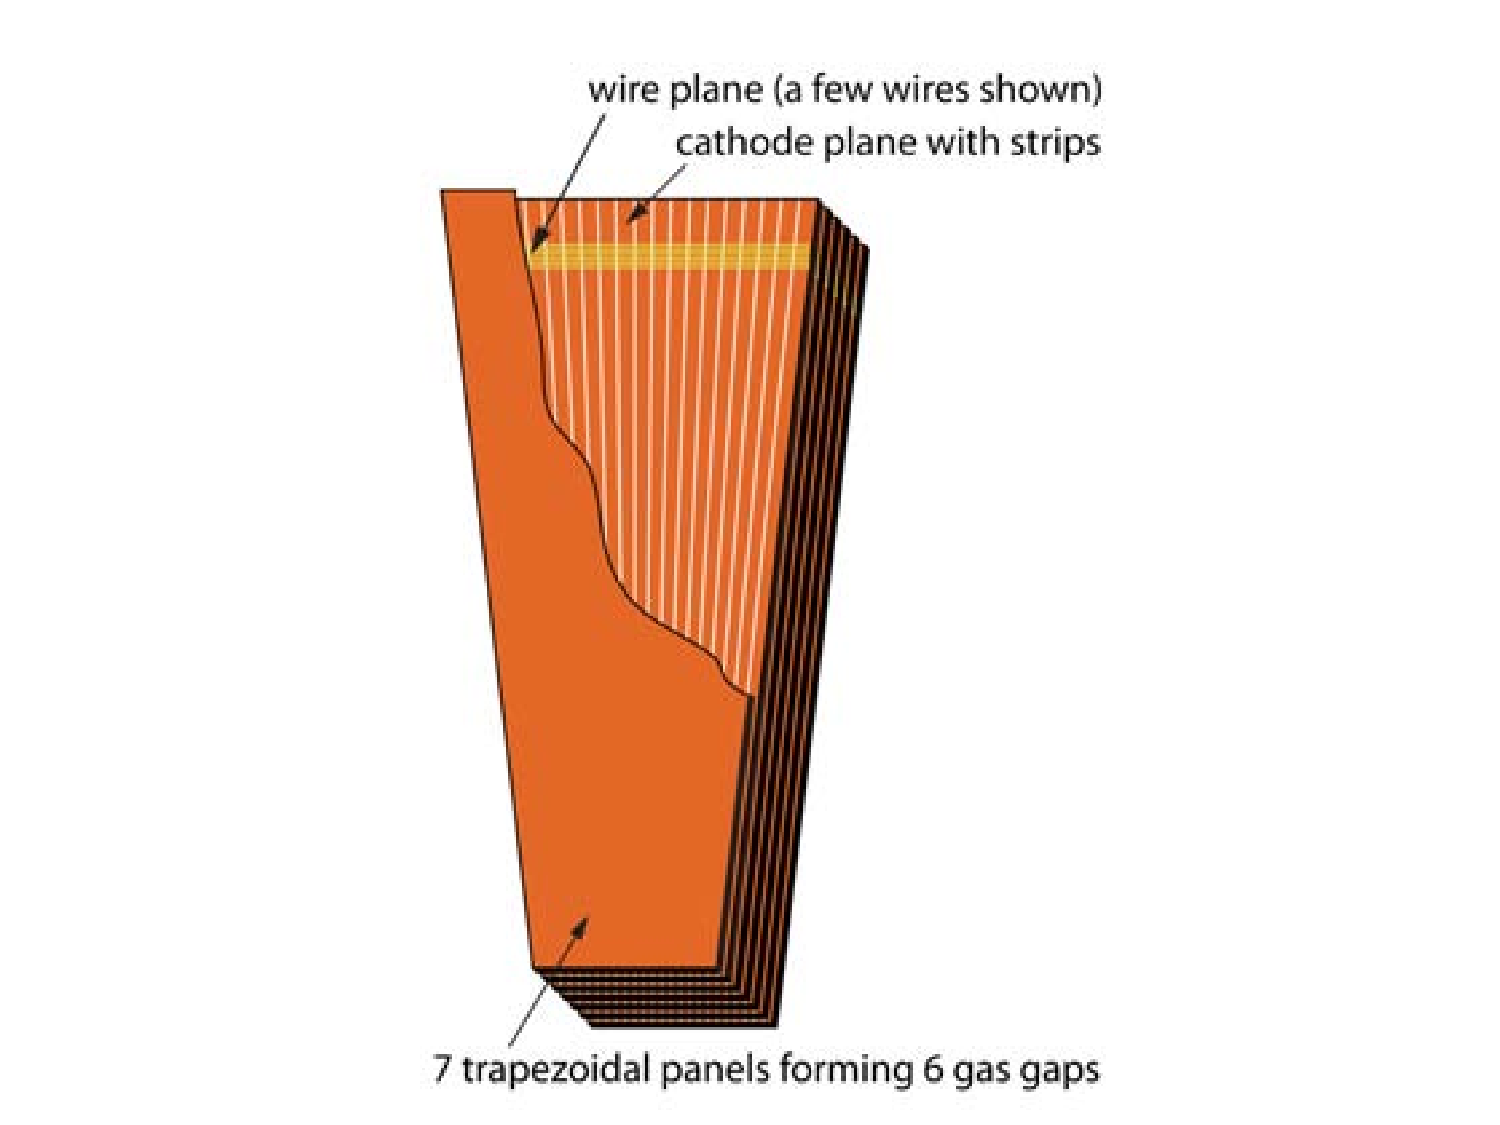
\includegraphics[width=0.6\textwidth]{Figures/CMS_Diagrams/Muon__CSC.pdf}
  \caption{A CSC station with 7 layers, making 6 gas chambers.
    Cathode strips are shown in yellow, perpendicular to the vertical
    anode wires in orange. } \label{fig:muon_csc_layout}
\end{figure}

\par In addition to RPCs, the muon endcap (ME) system, uses cathode
strip chambers (CSCs) to provide additional spatial resolution on
muons.  Each endcap has 4 layers of CSCs, with a trapezoidanal shape,
with 468 cathode strip chambers distrubed on each.  Three groups of 72
are located on the iner disk, a group of 36 and a group of 72 in the
second and third disk, and a group of 36 in the outer disk.  Figure
\ref{fig:muon_csc_layout} shows the layout of a quarter section of the
CSC system in the ME.  A CSC station consists of 6 layers of gas
chambers, where each chamber is an array of anode wires, held at a
positive voltage, arranged perpendicular to cathode strips, held at
negative voltage.  The volume of the chamber is filled with a gas that 
is 40$\%$ Argon, 50$\%$ CO$_{2}$, and 10$\%$ CF$_{4}$.  When a muon
passes through the volume, the gas is ionized, and now, since the
anode and cathode strips are perpendicular, when the electrons and gas
ions combine with the anode and cathode repsectively, a 2-D
measurement of the muon's position is recorded.  Figure
\ref{fig:muon_csc_layout} shows a diagram of a CSC chamber with 7
layers to create the 6 gas chambers.  

\section{Data Collection Overview}
\label{data_collection_description}

\par The LHC is designed to deliver protons at 40 MHz, corresponding
to a bunch crossing every 25 ns.  The majority of the interactions will
be glancing, low-energy collisions, which do little to reveal new
phenomenon, and would be impossible to store for analysis.  A trigger
system is designed to select interesting events with a large potential
of revealing new physics.  The rate is reduced in two steps through
the Level-1 (L1) trigger, and the High-Level Trigger (HLT).  The L1
trigger is composed of programmable electronics and hardware that
buffers the data and perform simple calculations on tracks and
calorimeter energy deposits to determine whether an event should be
kept for analysis.  This reduces the event rate from 40 MHz to 10
kHz.  The HLT is a computer farm of $\sim$1000 computer processors,
that perform a more sophisticated reconstruction of the tracks and
energy deposits, as well as more complicated calculations between
reconstructed objects.  This stage reduces the rate to a much more
manageable 100 Hz.    

\begin{figure}[h]
   \centering
  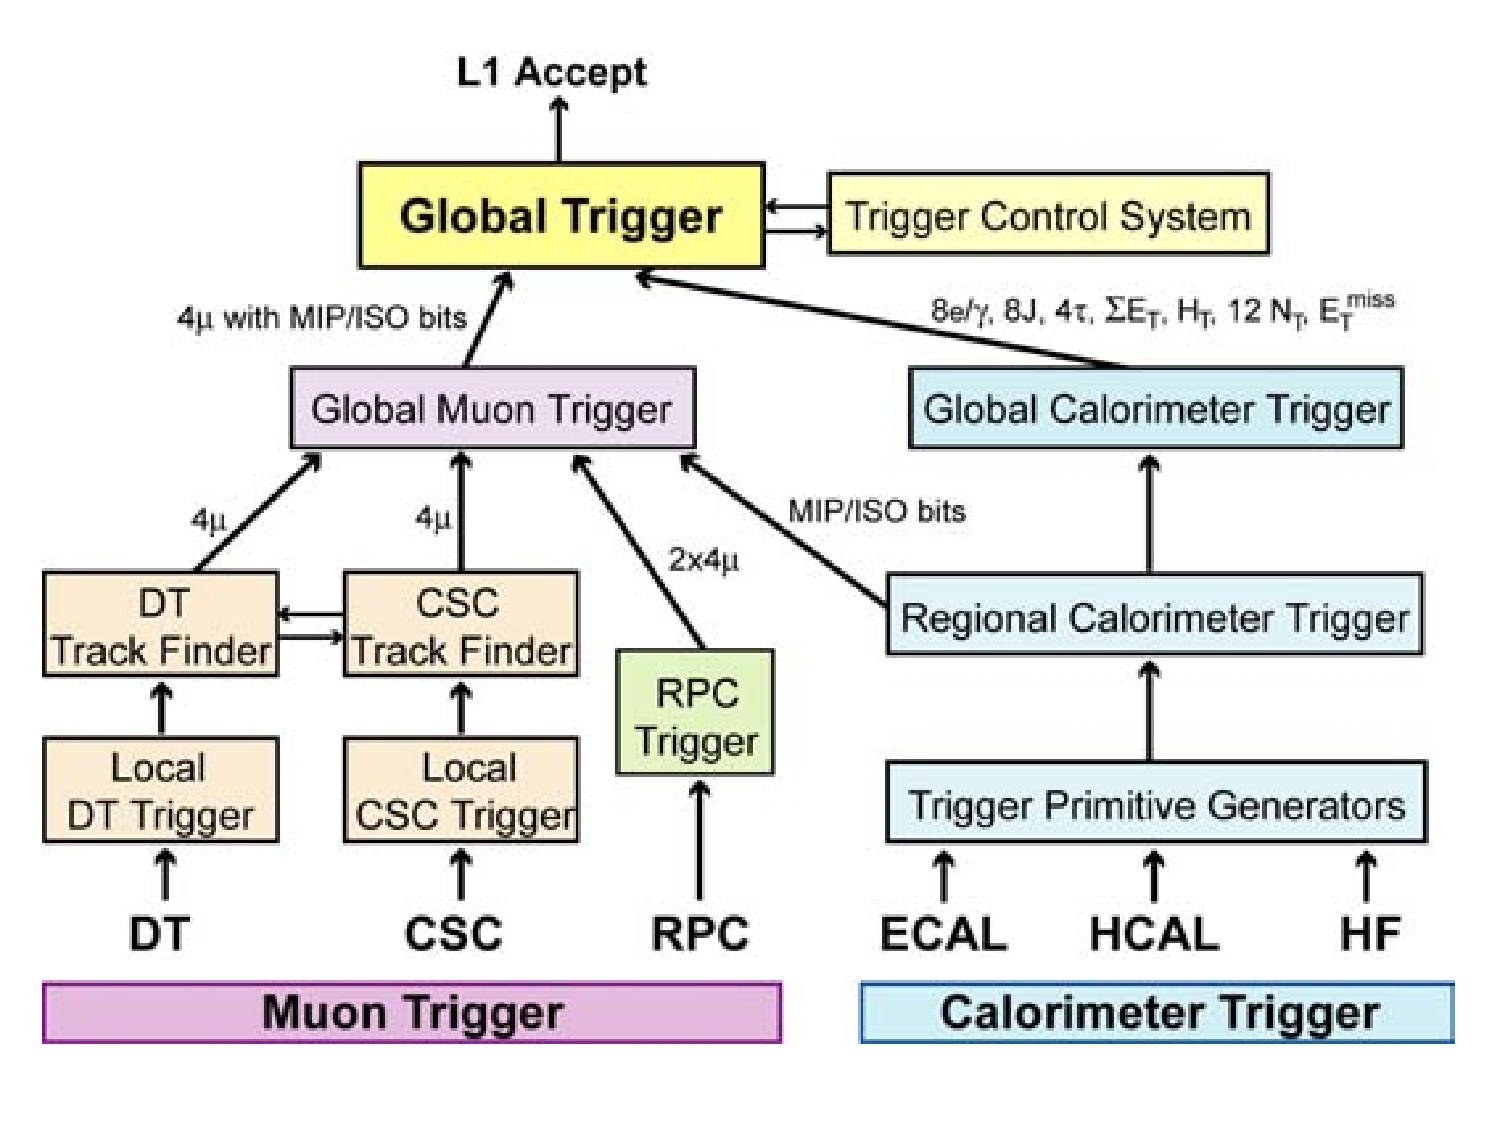
\includegraphics[width=0.6\textwidth]{Figures/CMS_Diagrams/Trigger__L1_layout.pdf}
  \caption{A block diagram of the L1 trigger}\label{fig:tigger_L1_layout}
\end{figure}

\par The L1 trigger is composed of local, regional, and global
components.  The process of determining whether to accept or reject
the event begins by calculating Trigger Primitive Generators (TPGs)
based on calorimeter energy deposits, and tracks in the muon
chambers.  The entire process has a latency time of 3.2 $\mu$s, which
corresponds to the length of the LHC abort gap.  Sufficiently large
data buffers allow the storage of all the events processed during a
bunch train, meaning that CMS is capable of running with zero dead
time due to detector readout latency.  

\par In the ECAL a trigger tower consists of a 5$\times$5 array
of crystals.  Front-end electronics on the crystals receive ADC counts
on the amplitudes of the photomultipliers, and uses information
encoded in the electronics to convert this sum to the transverse
energy, $\ET$ deposited in the crystals.  The EB TPG also encodes
information about the distribution of energy, and thus the shower
shape in the 5$\times$5 array, wich is used to veto anomolous
signals.  In the HCAL, a trigger tower consists of one of the 16
azimuthal wedges, with segmentation $(\Delta\eta, \Delta\phi) =
(0.087, 0.087)$, in the barrel and endcap.  Similarly to the ECAL,
front-end electronics digitize the signal from the HCAL HPDs, and
convert the ADC counts into sums of transverse energy.  These
calorimeter TPGs are sent to a Regional Calorimeter Trigger (RCT) that
is composed of a 4$\times$4 array of trigger towers, with the
exception of the HF, which is formed by a single trigger tower.

\begin{figure}[h]
   \centering
  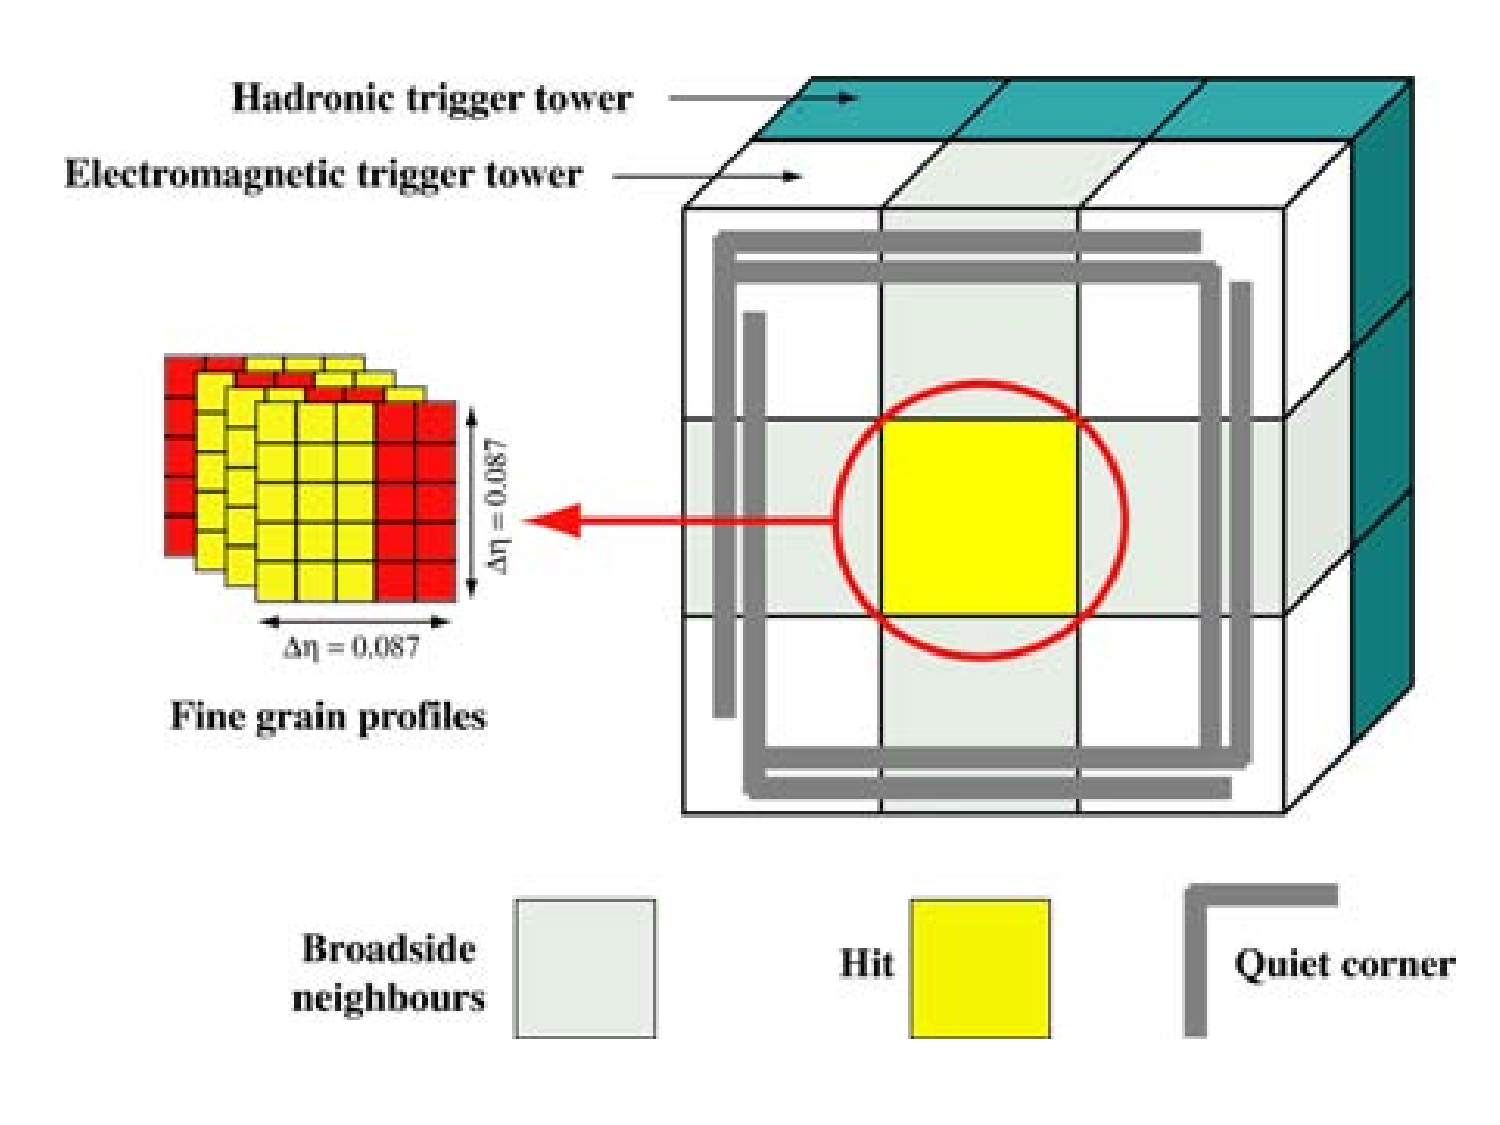
\includegraphics[width=0.6\textwidth]{Figures/CMS_Diagrams/Trigger__RCT_schematic.pdf}
  \caption{A schematic of the $e/\gamma$ trigger algorithm} \label{fig:tigger_rct_algo}
\end{figure}

\par The RCT determines electron and photon candidates from the
calorimeter sums.  The $e/\gamma$ trigger searches for the highest
energy trigger tower in the ECAL.  Within that trigger tower, it
checks that the EM shower is contained in a 2$\times$5 array of crystals
and that the ratio of ECAL to HCAL energies is less than 5$\%$.  It is
considered an isolated electron of all eight of its nesarest neighbors
pass these requirements, and a corner of five neighbors has energy
below a threshold requirement.  It is considered a non-isolated
electron if only the second highest $\ET$ broadside neighbor trigger
tower passes these critera.  Up to four isolated, and four
non-isolated $e/\gamma$ candidates per RCT are passed to the Global
Calorimeter Trigger (GCT).  

\par The GCT determines jets, total transverse energy, missing
transverse energy, jet counts, and $\HT$ (scalar sum of transverse
momentum), in addition to the highest rank isolated and non-isolated
$e\/gamma$ candidates.  Jets are found in a clustering algorithm that
looks for large energy deposits in 2$\times$12 cells of $\phi$ or
$\eta$ that span 40$^{\circ}$ and half the detector in each of
coordinates.  Up to four jets, and four tau jets from the HCAL and
four jets from the HF are forwarded to the Global Trigger (GT).  

 \par The non-calorimeter based triggers are based on measurements of
 the DTs, CSCs, and RPCs in the muon drift chambers.  The barrel DTs
 look for hit patterns among neighboring tubes in successvice layers,
 and fits a track segments in the $\eta$ and $\phi$ coordinates.  The
 endcap CSCs provde 3-dimensional track semgments and are combined
 with the DTs to form tracks that are passed to the Global Muon
 Trigger (GMT).  The RPCs provide an indpedent set of tracks and
 timing hits to the GMT.  Each bunch crossing the GMTs receive up to
 four muon candidates in the barrel RPCs, four from the barrel DTs,
 four from the endcap RPCs, and four from the endcap CSCs.  The GMT
 records the candidate's $\PT$, charge, $\eta$, and $\phi$ position,
 as well as a quality code related to the fit of the track to the hit
 positions of the detector.  The GMT sends then sends these muon
 candidates to the GT.  

\par The Global Trigger can execute up to 128 trigger algorithms in
parallel to analyze the $\PT$, charge, $\eta$, and $\phi$ position,
and associated quality codes for muons, electrons, photons, jets, and
missing transverse energy.  Most algorithms compare single object
characterstics to thresholds to determine if they pass minimally
interesting critera.  If any of the algorithms return a passing
decision, the L1 trigger issues an accept statement that allows the
data stored in buffers to be readout by the CMS Data Acquisition (DAQ)
system.  

\begin{figure}[h]
   \centering
  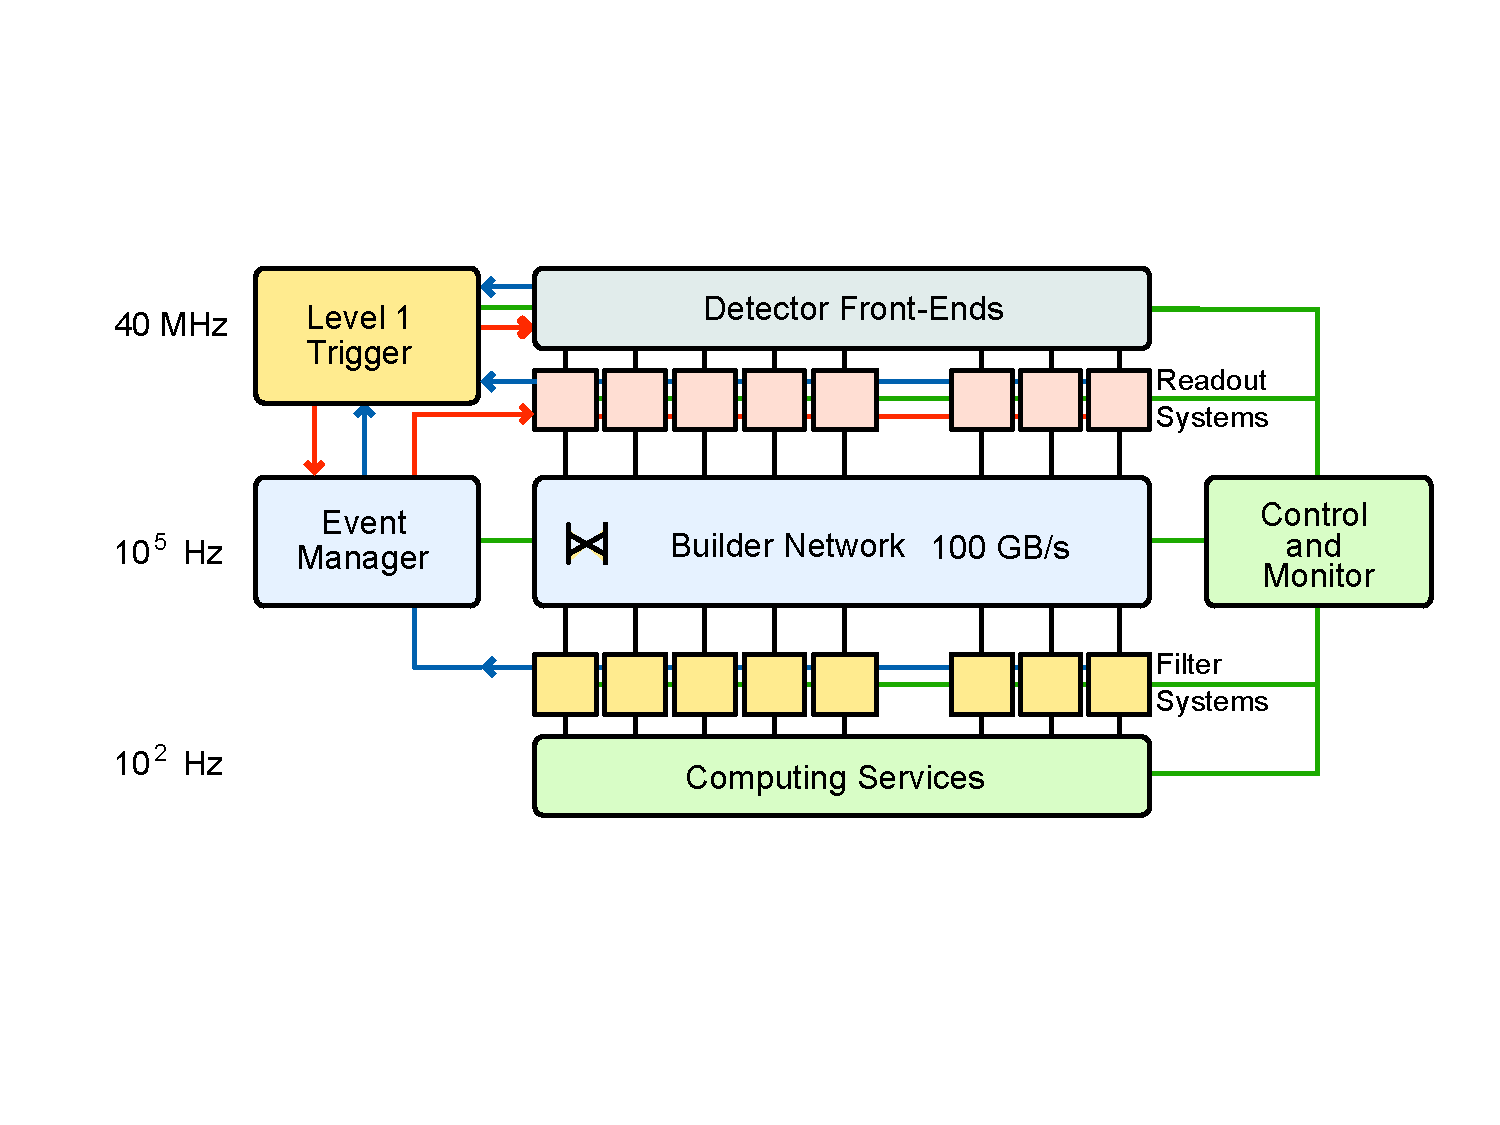
\includegraphics[width=0.6\textwidth]{Figures/CMS_Diagrams/Trigger__DAQ_layout.pdf}
  \caption{Layout of the CMS DAQ} \label{fig:tigger_daq}
\end{figure}

\par The CMS DAQ collects information fron 626 subdector Front End
Drivers (FEDs), which extract the buffered information from the
various front-end systems, upon the arrival of a L1 trigger accept.
An event builder algorithm assembles the framents from the various
sub-systems into a single coherent event, and transmits the
information to the HLT computing farms.  Figure \ref{fig:tigger_daq}
shows a schematic of the DAQ system.  

\par  The HLT computer farm performs the final reduction of data rate,
from 100kHz from the L1 to 100Hz.  The computer farm performs basic
consistency checks to ensure the quality of the data, then performs
calculations based on topology of the HLT path.  Typically, a more
sophisticated reconstruciton of an object takes place, and kinematic
cuts are applied to the object or in relationship to other objects in
the event.  Each HLT path forms its own data set, thus creating single
muon, single electron, electron+jets, etc. type datasets.  The upacked
detector information read by the DAQ is composed of ADC counts for
each readout channel, TPGs, and the L1 decsion.  This is known as the
RAW dataset.  Reconstructed physics objects are stored RECO data teir,
and finally an analysis object data (AOD) teir is created containing
only information about the reconstructed objects without having to
store detector information.  This last format requires the least
amount of data per event for storage, and contains the reconstructed
physics objects, such as electrons, muons, jets, etc. which are be
used to search for new physics phenomenom.  